\documentclass[twoside]{book}

% Packages required by doxygen
\usepackage{fixltx2e}
\usepackage{calc}
\usepackage{doxygen}
\usepackage[export]{adjustbox} % also loads graphicx
\usepackage{graphicx}
\usepackage[utf8]{inputenc}
\usepackage{makeidx}
\usepackage{multicol}
\usepackage{multirow}
\PassOptionsToPackage{warn}{textcomp}
\usepackage{textcomp}
\usepackage[nointegrals]{wasysym}
\usepackage[table]{xcolor}

% Font selection
\usepackage[T1]{fontenc}
\usepackage[scaled=.90]{helvet}
\usepackage{courier}
\usepackage{amssymb}
\usepackage{sectsty}
\renewcommand{\familydefault}{\sfdefault}
\allsectionsfont{%
  \fontseries{bc}\selectfont%
  \color{darkgray}%
}
\renewcommand{\DoxyLabelFont}{%
  \fontseries{bc}\selectfont%
  \color{darkgray}%
}
\newcommand{\+}{\discretionary{\mbox{\scriptsize$\hookleftarrow$}}{}{}}

% Page & text layout
\usepackage{geometry}
\geometry{%
  a4paper,%
  top=2.5cm,%
  bottom=2.5cm,%
  left=2.5cm,%
  right=2.5cm%
}
\tolerance=750
\hfuzz=15pt
\hbadness=750
\setlength{\emergencystretch}{15pt}
\setlength{\parindent}{0cm}
\setlength{\parskip}{3ex plus 2ex minus 2ex}
\makeatletter
\renewcommand{\paragraph}{%
  \@startsection{paragraph}{4}{0ex}{-1.0ex}{1.0ex}{%
    \normalfont\normalsize\bfseries\SS@parafont%
  }%
}
\renewcommand{\subparagraph}{%
  \@startsection{subparagraph}{5}{0ex}{-1.0ex}{1.0ex}{%
    \normalfont\normalsize\bfseries\SS@subparafont%
  }%
}
\makeatother

% Headers & footers
\usepackage{fancyhdr}
\pagestyle{fancyplain}
\fancyhead[LE]{\fancyplain{}{\bfseries\thepage}}
\fancyhead[CE]{\fancyplain{}{}}
\fancyhead[RE]{\fancyplain{}{\bfseries\leftmark}}
\fancyhead[LO]{\fancyplain{}{\bfseries\rightmark}}
\fancyhead[CO]{\fancyplain{}{}}
\fancyhead[RO]{\fancyplain{}{\bfseries\thepage}}
\fancyfoot[LE]{\fancyplain{}{}}
\fancyfoot[CE]{\fancyplain{}{}}
\fancyfoot[RE]{\fancyplain{}{\bfseries\scriptsize Generated by Doxygen }}
\fancyfoot[LO]{\fancyplain{}{\bfseries\scriptsize Generated by Doxygen }}
\fancyfoot[CO]{\fancyplain{}{}}
\fancyfoot[RO]{\fancyplain{}{}}
\renewcommand{\footrulewidth}{0.4pt}
\renewcommand{\chaptermark}[1]{%
  \markboth{#1}{}%
}
\renewcommand{\sectionmark}[1]{%
  \markright{\thesection\ #1}%
}

% Indices & bibliography
\usepackage{natbib}
\usepackage[titles]{tocloft}
\setcounter{tocdepth}{3}
\setcounter{secnumdepth}{5}
\makeindex

% Hyperlinks (required, but should be loaded last)
\usepackage{ifpdf}
\ifpdf
  \usepackage[pdftex,pagebackref=true]{hyperref}
\else
  \usepackage[ps2pdf,pagebackref=true]{hyperref}
\fi
\hypersetup{%
  colorlinks=true,%
  linkcolor=blue,%
  citecolor=blue,%
  unicode%
}

% Custom commands
\newcommand{\clearemptydoublepage}{%
  \newpage{\pagestyle{empty}\cleardoublepage}%
}

\usepackage{caption}
\captionsetup{labelsep=space,justification=centering,font={bf},singlelinecheck=off,skip=4pt,position=top}

%===== C O N T E N T S =====

\begin{document}

% Titlepage & ToC
\hypersetup{pageanchor=false,
             bookmarksnumbered=true,
             pdfencoding=unicode
            }
\pagenumbering{alph}
\begin{titlepage}
\vspace*{7cm}
\begin{center}%
{\Large Game Project }\\
\vspace*{1cm}
{\large Generated by Doxygen 1.8.13}\\
\end{center}
\end{titlepage}
\clearemptydoublepage
\pagenumbering{roman}
\tableofcontents
\clearemptydoublepage
\pagenumbering{arabic}
\hypersetup{pageanchor=true}

%--- Begin generated contents ---
\chapter{R\+E\+A\+D\+ME}
\label{md_README}
\Hypertarget{md_README}
\input{md_README}
\chapter{Data Structure Index}
\doxysection{Data Structures}
Here are the data structures with brief descriptions\+:\begin{DoxyCompactList}
\item\contentsline{section}{\mbox{\hyperlink{structenigme}{enigme}} }{\pageref{structenigme}}{}
\item\contentsline{section}{\mbox{\hyperlink{structennemi}{ennemi}} }{\pageref{structennemi}}{}
\item\contentsline{section}{\mbox{\hyperlink{structpersonnage}{personnage}} }{\pageref{structpersonnage}}{}
\item\contentsline{section}{\mbox{\hyperlink{structsaveFile}{save\+File}} }{\pageref{structsaveFile}}{}
\end{DoxyCompactList}

\chapter{File Index}
\doxysection{File List}
Here is a list of all files with brief descriptions\+:\begin{DoxyCompactList}
\item\contentsline{section}{\mbox{\hyperlink{defs_8c}{defs.\+c}} \\*Global variables }{\pageref{defs_8c}}{}
\item\contentsline{section}{\mbox{\hyperlink{defs_8h}{defs.\+h}} \\*Global variables definitions }{\pageref{defs_8h}}{}
\item\contentsline{section}{\mbox{\hyperlink{enigme_8c}{enigme.\+c}} \\*Riddle functions }{\pageref{enigme_8c}}{}
\item\contentsline{section}{\mbox{\hyperlink{enigme_8h}{enigme.\+h}} \\*Riddle struct and function prototypes }{\pageref{enigme_8h}}{}
\item\contentsline{section}{\mbox{\hyperlink{ennemies_8c}{ennemies.\+c}} \\*Game ennemies functions }{\pageref{ennemies_8c}}{}
\item\contentsline{section}{\mbox{\hyperlink{ennemies_8h}{ennemies.\+h}} \\*Ennemies struct and function prototypes }{\pageref{ennemies_8h}}{}
\item\contentsline{section}{\mbox{\hyperlink{gameplay_8c}{gameplay.\+c}} \\*In-\/game gameplay source code }{\pageref{gameplay_8c}}{}
\item\contentsline{section}{\mbox{\hyperlink{gameplay_8h}{gameplay.\+h}} \\*In-\/game function prototypes }{\pageref{gameplay_8h}}{}
\item\contentsline{section}{\mbox{\hyperlink{inits_8c}{inits.\+c}} \\*Initialisation functions implementation }{\pageref{inits_8c}}{}
\item\contentsline{section}{\mbox{\hyperlink{inits_8h}{inits.\+h}} \\*Initialization functions for the game }{\pageref{inits_8h}}{}
\item\contentsline{section}{\mbox{\hyperlink{main_8c}{main.\+c}} \\*Main program file }{\pageref{main_8c}}{}
\item\contentsline{section}{\mbox{\hyperlink{personnage_8c}{personnage.\+c}} \\*Game character functions implementation }{\pageref{personnage_8c}}{}
\item\contentsline{section}{\mbox{\hyperlink{personnage_8h}{personnage.\+h}} \\*Charcacter struct and function prototypes }{\pageref{personnage_8h}}{}
\item\contentsline{section}{\mbox{\hyperlink{ui_8c}{ui.\+c}} }{\pageref{ui_8c}}{}
\item\contentsline{section}{\mbox{\hyperlink{utils_8c}{utils.\+c}} }{\pageref{utils_8c}}{}
\item\contentsline{section}{\mbox{\hyperlink{utils_8h}{utils.\+h}} \\*Many utilities and helper functions }{\pageref{utils_8h}}{}
\end{DoxyCompactList}

\chapter{Data Structure Documentation}
\hypertarget{structenigme}{}\section{enigme Struct Reference}
\label{structenigme}\index{enigme@{enigme}}


{\ttfamily \#include $<$enigme.\+h$>$}

\subsection*{Data Fields}
\begin{DoxyCompactItemize}
\item 
int \hyperlink{structenigme_a2dfaa436eec08235e9d171809c885625}{type}
\item 
char \hyperlink{structenigme_ac5f266cc0f0376564e4707b072e9ed5e}{question} \mbox{[}60\mbox{]}
\item 
char \hyperlink{structenigme_acbdf1b2afa5727b3e237f0930df1038c}{reponses} \mbox{[}4\mbox{]}\mbox{[}60\mbox{]}
\item 
char \hyperlink{structenigme_ac5068c8be72169b27a39df8e82577b0d}{reponse}
\item 
int \hyperlink{structenigme_ab0fa044155e2331723b3a74822ccb6b0}{reponse\+Int}
\item 
int \hyperlink{structenigme_adb2a42545d9e64a26691b8ce4dc5341a}{a}
\item 
int \hyperlink{structenigme_a62f32d690aa699e921c0e8921573491e}{b}
\item 
S\+D\+L\+\_\+\+Surface $\ast$ \hyperlink{structenigme_a8c865bdd8e1c473935c4fa79e386c3cc}{enigme}
\item 
int \hyperlink{structenigme_a1e1e6c58f33ffed48b4eda090889ca38}{start\+Ticks}
\end{DoxyCompactItemize}


\subsection{Field Documentation}
\mbox{\Hypertarget{structenigme_adb2a42545d9e64a26691b8ce4dc5341a}\label{structenigme_adb2a42545d9e64a26691b8ce4dc5341a}} 
\index{enigme@{enigme}!a@{a}}
\index{a@{a}!enigme@{enigme}}
\subsubsection{\texorpdfstring{a}{a}}
{\footnotesize\ttfamily int enigme\+::a}

\mbox{\Hypertarget{structenigme_a62f32d690aa699e921c0e8921573491e}\label{structenigme_a62f32d690aa699e921c0e8921573491e}} 
\index{enigme@{enigme}!b@{b}}
\index{b@{b}!enigme@{enigme}}
\subsubsection{\texorpdfstring{b}{b}}
{\footnotesize\ttfamily int enigme\+::b}

\mbox{\Hypertarget{structenigme_a8c865bdd8e1c473935c4fa79e386c3cc}\label{structenigme_a8c865bdd8e1c473935c4fa79e386c3cc}} 
\index{enigme@{enigme}!enigme@{enigme}}
\index{enigme@{enigme}!enigme@{enigme}}
\subsubsection{\texorpdfstring{enigme}{enigme}}
{\footnotesize\ttfamily S\+D\+L\+\_\+\+Surface$\ast$ enigme\+::enigme}

\mbox{\Hypertarget{structenigme_ac5f266cc0f0376564e4707b072e9ed5e}\label{structenigme_ac5f266cc0f0376564e4707b072e9ed5e}} 
\index{enigme@{enigme}!question@{question}}
\index{question@{question}!enigme@{enigme}}
\subsubsection{\texorpdfstring{question}{question}}
{\footnotesize\ttfamily char enigme\+::question\mbox{[}60\mbox{]}}

\mbox{\Hypertarget{structenigme_ac5068c8be72169b27a39df8e82577b0d}\label{structenigme_ac5068c8be72169b27a39df8e82577b0d}} 
\index{enigme@{enigme}!reponse@{reponse}}
\index{reponse@{reponse}!enigme@{enigme}}
\subsubsection{\texorpdfstring{reponse}{reponse}}
{\footnotesize\ttfamily char enigme\+::reponse}

\mbox{\Hypertarget{structenigme_ab0fa044155e2331723b3a74822ccb6b0}\label{structenigme_ab0fa044155e2331723b3a74822ccb6b0}} 
\index{enigme@{enigme}!reponse\+Int@{reponse\+Int}}
\index{reponse\+Int@{reponse\+Int}!enigme@{enigme}}
\subsubsection{\texorpdfstring{reponse\+Int}{reponseInt}}
{\footnotesize\ttfamily int enigme\+::reponse\+Int}

\mbox{\Hypertarget{structenigme_acbdf1b2afa5727b3e237f0930df1038c}\label{structenigme_acbdf1b2afa5727b3e237f0930df1038c}} 
\index{enigme@{enigme}!reponses@{reponses}}
\index{reponses@{reponses}!enigme@{enigme}}
\subsubsection{\texorpdfstring{reponses}{reponses}}
{\footnotesize\ttfamily char enigme\+::reponses\mbox{[}4\mbox{]}\mbox{[}60\mbox{]}}

\mbox{\Hypertarget{structenigme_a1e1e6c58f33ffed48b4eda090889ca38}\label{structenigme_a1e1e6c58f33ffed48b4eda090889ca38}} 
\index{enigme@{enigme}!start\+Ticks@{start\+Ticks}}
\index{start\+Ticks@{start\+Ticks}!enigme@{enigme}}
\subsubsection{\texorpdfstring{start\+Ticks}{startTicks}}
{\footnotesize\ttfamily int enigme\+::start\+Ticks}

\mbox{\Hypertarget{structenigme_a2dfaa436eec08235e9d171809c885625}\label{structenigme_a2dfaa436eec08235e9d171809c885625}} 
\index{enigme@{enigme}!type@{type}}
\index{type@{type}!enigme@{enigme}}
\subsubsection{\texorpdfstring{type}{type}}
{\footnotesize\ttfamily int enigme\+::type}



The documentation for this struct was generated from the following file\+:\begin{DoxyCompactItemize}
\item 
\hyperlink{enigme_8h}{enigme.\+h}\end{DoxyCompactItemize}

\hypertarget{structennemi}{}\doxysection{ennemi Struct Reference}
\label{structennemi}\index{ennemi@{ennemi}}


struct for ennemi  




{\ttfamily \#include $<$ennemies.\+h$>$}

\doxysubsection*{Data Fields}
\begin{DoxyCompactItemize}
\item 
int \mbox{\hyperlink{structennemi_aa20d1f2c58368aa075a35cf5f2cad931}{posX}}
\item 
int \mbox{\hyperlink{structennemi_a4b6aa99c085e81e3dec2df8d985f957a}{posY}}
\item 
int \mbox{\hyperlink{structennemi_aaf749231f2819d6bd2c974e47712a483}{animation\+Frame}}
\item 
int \mbox{\hyperlink{structennemi_aa1f57a616910ffd5799f1097a3160e0b}{direction}}
\item 
S\+D\+L\+\_\+\+Surface $\ast$ \mbox{\hyperlink{structennemi_a6a5af0f9f9357971d04304b866b87d12}{current\+Frame}}
\item 
int \mbox{\hyperlink{structennemi_afd42e01f19c7fcec3cb21dca8b4cf346}{pos\+X\+Deb}}
\item 
int \mbox{\hyperlink{structennemi_a6da098ed49233503a361e3dbe184e3f4}{pos\+X\+Fin}}
\end{DoxyCompactItemize}


\doxysubsection{Detailed Description}
struct for ennemi 

\doxysubsection{Field Documentation}
\mbox{\Hypertarget{structennemi_aaf749231f2819d6bd2c974e47712a483}\label{structennemi_aaf749231f2819d6bd2c974e47712a483}} 
\index{ennemi@{ennemi}!animationFrame@{animationFrame}}
\index{animationFrame@{animationFrame}!ennemi@{ennemi}}
\doxysubsubsection{\texorpdfstring{animationFrame}{animationFrame}}
{\footnotesize\ttfamily int ennemi\+::animation\+Frame}

\mbox{\Hypertarget{structennemi_a6a5af0f9f9357971d04304b866b87d12}\label{structennemi_a6a5af0f9f9357971d04304b866b87d12}} 
\index{ennemi@{ennemi}!currentFrame@{currentFrame}}
\index{currentFrame@{currentFrame}!ennemi@{ennemi}}
\doxysubsubsection{\texorpdfstring{currentFrame}{currentFrame}}
{\footnotesize\ttfamily S\+D\+L\+\_\+\+Surface$\ast$ ennemi\+::current\+Frame}

\mbox{\Hypertarget{structennemi_aa1f57a616910ffd5799f1097a3160e0b}\label{structennemi_aa1f57a616910ffd5799f1097a3160e0b}} 
\index{ennemi@{ennemi}!direction@{direction}}
\index{direction@{direction}!ennemi@{ennemi}}
\doxysubsubsection{\texorpdfstring{direction}{direction}}
{\footnotesize\ttfamily int ennemi\+::direction}

\mbox{\Hypertarget{structennemi_aa20d1f2c58368aa075a35cf5f2cad931}\label{structennemi_aa20d1f2c58368aa075a35cf5f2cad931}} 
\index{ennemi@{ennemi}!posX@{posX}}
\index{posX@{posX}!ennemi@{ennemi}}
\doxysubsubsection{\texorpdfstring{posX}{posX}}
{\footnotesize\ttfamily int ennemi\+::posX}

\mbox{\Hypertarget{structennemi_afd42e01f19c7fcec3cb21dca8b4cf346}\label{structennemi_afd42e01f19c7fcec3cb21dca8b4cf346}} 
\index{ennemi@{ennemi}!posXDeb@{posXDeb}}
\index{posXDeb@{posXDeb}!ennemi@{ennemi}}
\doxysubsubsection{\texorpdfstring{posXDeb}{posXDeb}}
{\footnotesize\ttfamily int ennemi\+::pos\+X\+Deb}

\mbox{\Hypertarget{structennemi_a6da098ed49233503a361e3dbe184e3f4}\label{structennemi_a6da098ed49233503a361e3dbe184e3f4}} 
\index{ennemi@{ennemi}!posXFin@{posXFin}}
\index{posXFin@{posXFin}!ennemi@{ennemi}}
\doxysubsubsection{\texorpdfstring{posXFin}{posXFin}}
{\footnotesize\ttfamily int ennemi\+::pos\+X\+Fin}

\mbox{\Hypertarget{structennemi_a4b6aa99c085e81e3dec2df8d985f957a}\label{structennemi_a4b6aa99c085e81e3dec2df8d985f957a}} 
\index{ennemi@{ennemi}!posY@{posY}}
\index{posY@{posY}!ennemi@{ennemi}}
\doxysubsubsection{\texorpdfstring{posY}{posY}}
{\footnotesize\ttfamily int ennemi\+::posY}



The documentation for this struct was generated from the following file\+:\begin{DoxyCompactItemize}
\item 
\mbox{\hyperlink{ennemies_8h}{ennemies.\+h}}\end{DoxyCompactItemize}

\hypertarget{structpersonnage}{}\doxysection{personnage Struct Reference}
\label{structpersonnage}\index{personnage@{personnage}}


{\ttfamily \#include $<$personnage.\+h$>$}

\doxysubsection*{Data Fields}
\begin{DoxyCompactItemize}
\item 
int \mbox{\hyperlink{structpersonnage_acb8e0ece93e2c7c15a1672e2867edc19}{speed}}
\item 
int \mbox{\hyperlink{structpersonnage_a6f803343f258e12f2c7127b405ff7ecb}{posX}}
\item 
int \mbox{\hyperlink{structpersonnage_afa542266546b567ffcaa7ead5dd0d3b5}{posY}}
\item 
int \mbox{\hyperlink{structpersonnage_a994136f5b53ed985410bac0afa02749c}{animation\+Frame}}
\item 
int \mbox{\hyperlink{structpersonnage_a2664acffa6fccd8487b9e03b63fbd6da}{direction}}
\item 
S\+D\+L\+\_\+\+Surface $\ast$ \mbox{\hyperlink{structpersonnage_a1b46abccb551fa81f64377bac4626b3a}{current\+Frame}}
\item 
int \mbox{\hyperlink{structpersonnage_a6590b4624503a2a0eb69c111d05debc2}{model}}
\item 
int \mbox{\hyperlink{structpersonnage_ad149509f75e8aff1950b313aab0d7888}{acceleration}}
\item 
int \mbox{\hyperlink{structpersonnage_a0d3b31e5b093c4c7befc15bceac92f7a}{max\+Speed}}
\item 
int \mbox{\hyperlink{structpersonnage_a84a5f30f7036e023aef06c14dd3ff5da}{current\+Speed}}
\item 
int \mbox{\hyperlink{structpersonnage_a6729ea8dd5e255a8597d8a76cdf05148}{reset\+Speed}}
\end{DoxyCompactItemize}


\doxysubsection{Field Documentation}
\mbox{\Hypertarget{structpersonnage_ad149509f75e8aff1950b313aab0d7888}\label{structpersonnage_ad149509f75e8aff1950b313aab0d7888}} 
\index{personnage@{personnage}!acceleration@{acceleration}}
\index{acceleration@{acceleration}!personnage@{personnage}}
\doxysubsubsection{\texorpdfstring{acceleration}{acceleration}}
{\footnotesize\ttfamily int personnage\+::acceleration}

\mbox{\Hypertarget{structpersonnage_a994136f5b53ed985410bac0afa02749c}\label{structpersonnage_a994136f5b53ed985410bac0afa02749c}} 
\index{personnage@{personnage}!animationFrame@{animationFrame}}
\index{animationFrame@{animationFrame}!personnage@{personnage}}
\doxysubsubsection{\texorpdfstring{animationFrame}{animationFrame}}
{\footnotesize\ttfamily int personnage\+::animation\+Frame}

\mbox{\Hypertarget{structpersonnage_a1b46abccb551fa81f64377bac4626b3a}\label{structpersonnage_a1b46abccb551fa81f64377bac4626b3a}} 
\index{personnage@{personnage}!currentFrame@{currentFrame}}
\index{currentFrame@{currentFrame}!personnage@{personnage}}
\doxysubsubsection{\texorpdfstring{currentFrame}{currentFrame}}
{\footnotesize\ttfamily S\+D\+L\+\_\+\+Surface$\ast$ personnage\+::current\+Frame}

\mbox{\Hypertarget{structpersonnage_a84a5f30f7036e023aef06c14dd3ff5da}\label{structpersonnage_a84a5f30f7036e023aef06c14dd3ff5da}} 
\index{personnage@{personnage}!currentSpeed@{currentSpeed}}
\index{currentSpeed@{currentSpeed}!personnage@{personnage}}
\doxysubsubsection{\texorpdfstring{currentSpeed}{currentSpeed}}
{\footnotesize\ttfamily int personnage\+::current\+Speed}

\mbox{\Hypertarget{structpersonnage_a2664acffa6fccd8487b9e03b63fbd6da}\label{structpersonnage_a2664acffa6fccd8487b9e03b63fbd6da}} 
\index{personnage@{personnage}!direction@{direction}}
\index{direction@{direction}!personnage@{personnage}}
\doxysubsubsection{\texorpdfstring{direction}{direction}}
{\footnotesize\ttfamily int personnage\+::direction}

\mbox{\Hypertarget{structpersonnage_a0d3b31e5b093c4c7befc15bceac92f7a}\label{structpersonnage_a0d3b31e5b093c4c7befc15bceac92f7a}} 
\index{personnage@{personnage}!maxSpeed@{maxSpeed}}
\index{maxSpeed@{maxSpeed}!personnage@{personnage}}
\doxysubsubsection{\texorpdfstring{maxSpeed}{maxSpeed}}
{\footnotesize\ttfamily int personnage\+::max\+Speed}

\mbox{\Hypertarget{structpersonnage_a6590b4624503a2a0eb69c111d05debc2}\label{structpersonnage_a6590b4624503a2a0eb69c111d05debc2}} 
\index{personnage@{personnage}!model@{model}}
\index{model@{model}!personnage@{personnage}}
\doxysubsubsection{\texorpdfstring{model}{model}}
{\footnotesize\ttfamily int personnage\+::model}

\mbox{\Hypertarget{structpersonnage_a6f803343f258e12f2c7127b405ff7ecb}\label{structpersonnage_a6f803343f258e12f2c7127b405ff7ecb}} 
\index{personnage@{personnage}!posX@{posX}}
\index{posX@{posX}!personnage@{personnage}}
\doxysubsubsection{\texorpdfstring{posX}{posX}}
{\footnotesize\ttfamily int personnage\+::posX}

\mbox{\Hypertarget{structpersonnage_afa542266546b567ffcaa7ead5dd0d3b5}\label{structpersonnage_afa542266546b567ffcaa7ead5dd0d3b5}} 
\index{personnage@{personnage}!posY@{posY}}
\index{posY@{posY}!personnage@{personnage}}
\doxysubsubsection{\texorpdfstring{posY}{posY}}
{\footnotesize\ttfamily int personnage\+::posY}

\mbox{\Hypertarget{structpersonnage_a6729ea8dd5e255a8597d8a76cdf05148}\label{structpersonnage_a6729ea8dd5e255a8597d8a76cdf05148}} 
\index{personnage@{personnage}!resetSpeed@{resetSpeed}}
\index{resetSpeed@{resetSpeed}!personnage@{personnage}}
\doxysubsubsection{\texorpdfstring{resetSpeed}{resetSpeed}}
{\footnotesize\ttfamily int personnage\+::reset\+Speed}

\mbox{\Hypertarget{structpersonnage_acb8e0ece93e2c7c15a1672e2867edc19}\label{structpersonnage_acb8e0ece93e2c7c15a1672e2867edc19}} 
\index{personnage@{personnage}!speed@{speed}}
\index{speed@{speed}!personnage@{personnage}}
\doxysubsubsection{\texorpdfstring{speed}{speed}}
{\footnotesize\ttfamily int personnage\+::speed}



The documentation for this struct was generated from the following file\+:\begin{DoxyCompactItemize}
\item 
\mbox{\hyperlink{personnage_8h}{personnage.\+h}}\end{DoxyCompactItemize}

\chapter{File Documentation}
\hypertarget{defs_8c}{}\doxysection{defs.\+c File Reference}
\label{defs_8c}\index{defs.c@{defs.c}}


global variables  


{\ttfamily \#include \char`\"{}defs.\+h\char`\"{}}\newline
Include dependency graph for defs.\+c\+:\nopagebreak
\begin{figure}[H]
\begin{center}
\leavevmode
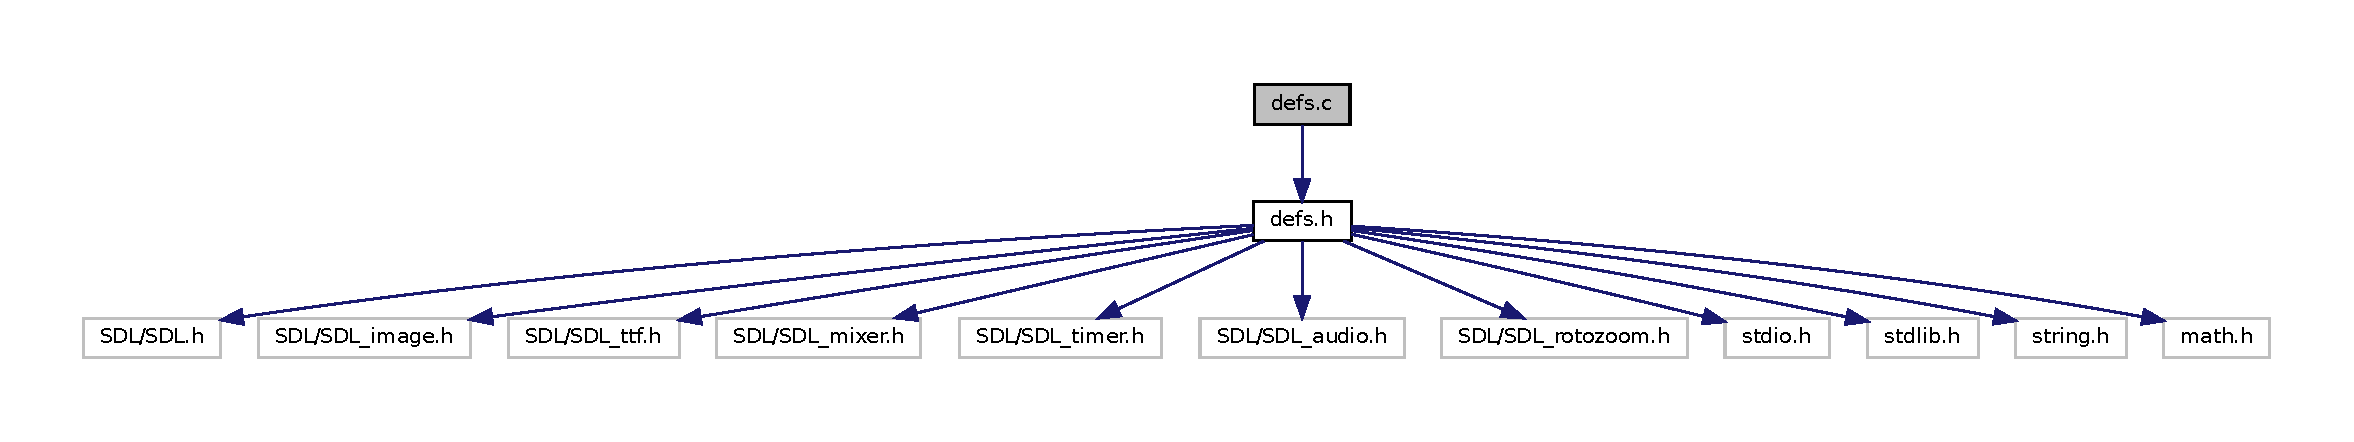
\includegraphics[width=350pt]{defs_8c__incl}
\end{center}
\end{figure}
\doxysubsection*{Variables}
\begin{DoxyCompactItemize}
\item 
S\+D\+L\+\_\+\+Surface $\ast$ \mbox{\hyperlink{defs_8c_a8a0695f3eaccf4eec9186f32ec831f20}{hello}}
\item 
S\+D\+L\+\_\+\+Surface $\ast$ \mbox{\hyperlink{defs_8c_a78fa3957d73de49cb81d047857504218}{screen}}
\item 
S\+D\+L\+\_\+\+Surface $\ast$ \mbox{\hyperlink{defs_8c_a78ab7f4978e38e13edc4a80caf138817}{message}}
\item 
S\+D\+L\+\_\+\+Surface $\ast$ \mbox{\hyperlink{defs_8c_a68389876c2746622931d187c587f9c4d}{background}}
\item 
S\+D\+L\+\_\+\+Surface $\ast$ \mbox{\hyperlink{defs_8c_aa73601f944838ffac2fa4d3e298a6ef4}{image}}
\item 
S\+D\+L\+\_\+\+Event \mbox{\hyperlink{defs_8c_a6b57f01d3c576db5368dd0efc2f435a4}{event}}
\item 
T\+T\+F\+\_\+\+Font $\ast$ \mbox{\hyperlink{defs_8c_abf5bfa705e66ffc1ddaa6ce46c960873}{font}}
\item 
S\+D\+L\+\_\+\+Color \mbox{\hyperlink{defs_8c_a631bf4babe4c1825a2cdc0c19c2bd04f}{color}}
\item 
S\+D\+L\+\_\+\+Surface $\ast$ \mbox{\hyperlink{defs_8c_a603a0f6fe738992cfe8f14c4360a0e4e}{buttons}}
\item 
Uint32 \mbox{\hyperlink{defs_8c_a0822b2f34b0cd24fc0a18aa2a73ee771}{next\+\_\+time}}
\item 
int \mbox{\hyperlink{defs_8c_adc359d0ba0a207e69da999c40bf762c8}{fullscreen}} = 0
\item 
S\+D\+L\+\_\+\+Surface $\ast$ \mbox{\hyperlink{defs_8c_a886ac8c83a9dd60d8ce8ea56b75237eb}{volume\+Surface}}
\item 
S\+D\+L\+\_\+\+Surface $\ast$ \mbox{\hyperlink{defs_8c_ae04cc1d68ad94e4a3b9b86bed1e6bff5}{window\+State}}
\item 
S\+D\+L\+\_\+\+Surface $\ast$ \mbox{\hyperlink{defs_8c_aa345627708064725e35e666a540c6c91}{volume\+Bar}}
\item 
S\+D\+L\+\_\+\+Surface $\ast$ \mbox{\hyperlink{defs_8c_a89a3c2e9ba42e8d59258ecb6888d939f}{volume\+Selector}}
\item 
S\+D\+L\+\_\+\+Surface $\ast$ \mbox{\hyperlink{defs_8c_a0c458e8109c971846c50a2a1e467bdb8}{menu\+Background}}
\item 
S\+D\+L\+\_\+\+Surface $\ast$ \mbox{\hyperlink{defs_8c_acb8cf8a5a0ecc8929eb27322a5915fe0}{menu\+Button\+Normal\+State}}
\item 
S\+D\+L\+\_\+\+Surface $\ast$ \mbox{\hyperlink{defs_8c_a5f92b0799599a11b310d0446efb34eed}{menu\+Button\+Clicked\+State}}
\item 
S\+D\+L\+\_\+\+Surface $\ast$ \mbox{\hyperlink{defs_8c_a29357cdf723f9f1d688a89fc9297c5df}{info\+Bar}}
\item 
S\+D\+L\+\_\+\+Surface $\ast$ \mbox{\hyperlink{defs_8c_af40d2934209209a2bbdfc52395907442}{slider}}
\item 
S\+D\+L\+\_\+\+Surface $\ast$ \mbox{\hyperlink{defs_8c_a5026584637c9ab6c7453b6d06e7a8865}{slider\+Bar}}
\item 
int \mbox{\hyperlink{defs_8c_a85ea1b63086b31a15d3ed2579c5715a6}{mouseX}}
\item 
int \mbox{\hyperlink{defs_8c_a3637abebcaa9d04aa18b1610d0921e16}{mouseY}}
\item 
char \mbox{\hyperlink{defs_8c_ad1b99a8251e9e08198dd7d58712559d1}{window\+State\+Char}} \mbox{[}15\mbox{]} = \char`\"{}Windowed\char`\"{}
\item 
S\+D\+L\+\_\+\+Surface $\ast$ \mbox{\hyperlink{defs_8c_ad22b3675c08f804b780be12b3d483c5f}{menu1}}
\item 
S\+D\+L\+\_\+\+Surface $\ast$ \mbox{\hyperlink{defs_8c_a417af12e04f849503ec50a1099905643}{menu2}}
\item 
S\+D\+L\+\_\+\+Surface $\ast$ \mbox{\hyperlink{defs_8c_a383dfb93f909d01760862403062962cc}{menu3}}
\item 
S\+D\+L\+\_\+\+Surface $\ast$ \mbox{\hyperlink{defs_8c_a18c72f024a1ea52461c5bdb3de91160b}{menu1\+Hover}}
\item 
S\+D\+L\+\_\+\+Surface $\ast$ \mbox{\hyperlink{defs_8c_ac61087fdd9269af636cd1bbfe69f66f0}{menu2\+Hover}}
\item 
S\+D\+L\+\_\+\+Surface $\ast$ \mbox{\hyperlink{defs_8c_ad0ae66eca85729f4a116652267974f1e}{menu3\+Hover}}
\item 
S\+D\+L\+\_\+\+Surface $\ast$ \mbox{\hyperlink{defs_8c_a0ac209296e33ac5089c4a4a5d3ee4b71}{new\+Game\+Button}}
\item 
S\+D\+L\+\_\+\+Surface $\ast$ \mbox{\hyperlink{defs_8c_ace1af332d79a0b6a47e8c597c1028776}{settings\+Button}}
\item 
S\+D\+L\+\_\+\+Surface $\ast$ \mbox{\hyperlink{defs_8c_a69599d632161dfcb6f030e1db3d8eed5}{quit\+Button}}
\item 
int \mbox{\hyperlink{defs_8c_a319f148f98ab6e78d52e318f4ce0c4f7}{fx\+Volume}} = 100
\item 
S\+D\+L\+\_\+\+Video\+Info $\ast$ \mbox{\hyperlink{defs_8c_a6745d0229f9912901115e5317589a6af}{info}}
\item 
int \mbox{\hyperlink{defs_8c_a2d4592ccdd56a3f524dc0a6f1ac2e10c}{play\+State}} = 0
\item 
int \mbox{\hyperlink{defs_8c_a77bd4f876bdc3afed5acdd936f775d34}{seconds}} = 0
\item 
\mbox{\hyperlink{defs_8h_abf38e439d63c2001b8bbb96dbab1bd86}{State}} \mbox{\hyperlink{defs_8c_a876b486d3a5241a126bd5751c5f70f79}{state}} = \mbox{\hyperlink{defs_8h_a44dd1b46a3f55007e78fc1ac506153b9}{M\+A\+I\+N\+\_\+\+M\+E\+NU}}
\item 
S\+D\+L\+\_\+\+Color \mbox{\hyperlink{defs_8c_a355224f147f9e7c339a0b8758b349e12}{selected}}
\item 
S\+D\+L\+\_\+\+Color \mbox{\hyperlink{defs_8c_aa22a61780b279c453d06c92453d0fcf6}{n\+\_\+selected}}
\item 
S\+D\+L\+\_\+\+Surface $\ast$ \mbox{\hyperlink{defs_8c_abf63c96eaa5561e71eb0449c2485bc2d}{settings\+Text}}
\item 
S\+D\+L\+\_\+\+Surface $\ast$ \mbox{\hyperlink{defs_8c_ad9406ab79432c083dcb1957c8e5cda1d}{mode\+Text}}
\item 
S\+D\+L\+\_\+\+Surface $\ast$ \mbox{\hyperlink{defs_8c_a2daf8dd43d6c903576b69a36f87c634e}{full\+Screen\+Text}}
\item 
S\+D\+L\+\_\+\+Surface $\ast$ \mbox{\hyperlink{defs_8c_a89e33cac9585c151579a15753d98d5c9}{windowed\+Text}}
\item 
S\+D\+L\+\_\+\+Surface $\ast$ \mbox{\hyperlink{defs_8c_a5fed5a0a1d1c7bc2e6affebfb59fe08d}{volume\+Text}}
\item 
S\+D\+L\+\_\+\+Surface $\ast$ \mbox{\hyperlink{defs_8c_ad2f52297bb83f45d2b276e17c22ad26d}{exit\+Text}}
\item 
Mix\+\_\+\+Music $\ast$ \mbox{\hyperlink{defs_8c_ab203ceba3699c997bf63f13bbc33b33a}{music}}
\item 
Mix\+\_\+\+Chunk $\ast$ \mbox{\hyperlink{defs_8c_a15b3213f20a453c753efb99f468778b7}{click}}
\item 
Mix\+\_\+\+Chunk $\ast$ \mbox{\hyperlink{defs_8c_af6976f3ff02b82755e3db73f9b3f93d9}{switcher}}
\item 
Mix\+\_\+\+Chunk $\ast$ \mbox{\hyperlink{defs_8c_a54c5edf6278e0284f9782bc30e46f21e}{fullscreen\+Sound}}
\item 
S\+D\+L\+\_\+\+Surface $\ast$ \mbox{\hyperlink{defs_8c_ad14ab720642740edf16e57f6c28ddbc9}{animation}}
\item 
int \mbox{\hyperlink{defs_8c_a27ed86ba911d1fc92308b64374dff8d6}{fullscreen\+Width}} = 0
\item 
int \mbox{\hyperlink{defs_8c_a1f4b1ad6932d7a03cfba053932dce53b}{fullscreen\+Height}} = 0
\item 
S\+D\+L\+\_\+\+Surface $\ast$ \mbox{\hyperlink{defs_8c_a0e03c4cc167dd7497007f1f3c8428f8a}{text1}}
\item 
S\+D\+L\+\_\+\+Surface $\ast$ \mbox{\hyperlink{defs_8c_acca77e0d07ce5db9ee27d900edf2bc93}{text2}}
\item 
S\+D\+L\+\_\+\+Surface $\ast$ \mbox{\hyperlink{defs_8c_af40006e8d3fb763f7ec6cc74a9d83f5d}{text3}}
\item 
int \mbox{\hyperlink{defs_8c_a45b3f1043a3b9217256cdb2129b7a0c4}{F\+PS}} = 30
\item 
int \mbox{\hyperlink{defs_8c_a93072262778c750b1245b6a70298ceeb}{music\+Volume}} = 0
\item 
int \mbox{\hyperlink{defs_8c_ad30f972f2e6e3e5ecab0dee38ae6cdb8}{frame}} = 1
\item 
int \mbox{\hyperlink{defs_8c_a2896431d6a80cd39b3d24b40237612ee}{quit}} = 0
\item 
int \mbox{\hyperlink{defs_8c_a2c910ea1a2e2fd5d8b1bc80210ec26c1}{menu\+Select}} = 0
\item 
int \mbox{\hyperlink{defs_8c_af9af62c53df614f4a9b08e76938d340f}{key\+Pressed}} = 0
\item 
int \mbox{\hyperlink{defs_8c_ab5fd9003c5db26855fcce82ddc169de3}{settings\+State}} = 0
\item 
int \mbox{\hyperlink{defs_8c_ac55d1466a0e202c7abb8ef4c1b1a0a23}{volume\+Slider}} = 0
\item 
int \mbox{\hyperlink{defs_8c_a0ebc172bfb7854a6d992f3ee7636ec9b}{inits}} = 0
\item 
S\+D\+L\+\_\+\+Surface $\ast$ \mbox{\hyperlink{defs_8c_a9dad4b780f049b0805f1000ebc312d8e}{game\+Background}}
\item 
S\+D\+L\+\_\+\+Surface $\ast$ \mbox{\hyperlink{defs_8c_a0ad344d281689f5b9f026a32af35a3d2}{game\+Background\+Mask}}
\item 
int \mbox{\hyperlink{defs_8c_ac68cd86607699f547cfa3ba4b3a4dfe5}{offset\+BG}} = 0
\item 
int \mbox{\hyperlink{defs_8c_aef160b7437d94056f1dc59646cd5b87d}{score}} = 500
\item 
int \mbox{\hyperlink{defs_8c_a7a0ba9e8c59a789d927afb3d70583403}{vies}} = 3
\item 
int \mbox{\hyperlink{defs_8c_a5bac6ce7bdac65c6d16d68a2748f3cf4}{offset\+B\+G2}} = 0
\item 
int \mbox{\hyperlink{defs_8c_a19003dffcafa65c735195a37a300ac7c}{score2}} = 500
\item 
int \mbox{\hyperlink{defs_8c_aeacbe4abd5b202a06097681fce4a5175}{vies2}} = 3
\item 
S\+D\+L\+\_\+\+Surface $\ast$ \mbox{\hyperlink{defs_8c_a6c3f982896f92b962f6f61f17df23e52}{enigme\+Temp\+Image}}
\item 
int \mbox{\hyperlink{defs_8c_a27253d4a774a08a221ce3ddc7aab2ef5}{gameplay\+Start\+Tick}}
\item 
S\+D\+L\+\_\+\+Surface $\ast$ \mbox{\hyperlink{defs_8c_af6b74399e0c3c99b57533d663f4ed93d}{minimap}}
\item 
S\+D\+L\+\_\+\+Surface $\ast$ \mbox{\hyperlink{defs_8c_a000edb0bdaf3c5e7ada63c4a836beabc}{minimap\+Icon}}
\item 
int \mbox{\hyperlink{defs_8c_a1cb949030ab1a10f032df5c8c9651da8}{pos\+Xminimap\+Icon}}
\item 
int \mbox{\hyperlink{defs_8c_a89da1f31799de99df088690d2e53be1d}{pos\+Yminimap\+Icon}}
\item 
S\+D\+L\+\_\+\+Surface $\ast$ \mbox{\hyperlink{defs_8c_af45914eb8693af42c3f6d74bc65e597e}{selection\+Text1}}
\item 
S\+D\+L\+\_\+\+Surface $\ast$ \mbox{\hyperlink{defs_8c_a04e6b5a734cf4cf4f1f108d069fe4707}{selection\+Text2}}
\item 
S\+D\+L\+\_\+\+Surface $\ast$ \mbox{\hyperlink{defs_8c_a5f3f2ff27be4317ee86172945b8e0114}{selection\+Text3}}
\item 
S\+D\+L\+\_\+\+Surface $\ast$ \mbox{\hyperlink{defs_8c_a6a61b34e1ea565c8021aa042fc5e77eb}{selection\+Text4}}
\item 
S\+D\+L\+\_\+\+Surface $\ast$ \mbox{\hyperlink{defs_8c_a3ca9db829d6e3009ca07680a9fbd61dc}{selection\+Text5}}
\item 
S\+D\+L\+\_\+\+Surface $\ast$ \mbox{\hyperlink{defs_8c_a1272cae80057c3bf14d2567101d2068f}{selection\+Text6}}
\item 
S\+D\+L\+\_\+\+Surface $\ast$ \mbox{\hyperlink{defs_8c_ab9a8477dae6f8f4fc445f8f02de226ff}{selection\+Text7}}
\item 
int \mbox{\hyperlink{defs_8c_a251959219002530b57e690966c164ba1}{model\+Selected}}
\item 
int \mbox{\hyperlink{defs_8c_a186fa24cbaf490c50522cbbfce042849}{choice\+Select}} = -\/1
\item 
int \mbox{\hyperlink{defs_8c_a1fee669d4ceeaff15a54ed0daa1a1619}{game\+Selector}} = 1
\item 
int \mbox{\hyperlink{defs_8c_a7c8a8638b0f5c50f1bac3faa49c65de0}{chosen\+Mode}} = -\/1
\item 
int \mbox{\hyperlink{defs_8c_aa04c92cce8d193a69872f186e7a0e00e}{in\+Save\+Menu}} = 0
\item 
int \mbox{\hyperlink{defs_8c_a67b41426d82bc5ec5475a00071340df4}{save\+Menu\+Selector}}
\item 
int \mbox{\hyperlink{defs_8c_a40fe89b04b17671dad27eec3515ad6a2}{selected\+Save\+Menu}}
\end{DoxyCompactItemize}


\doxysubsection{Detailed Description}
global variables 

\begin{DoxyAuthor}{Author}
Creative Sparks 
\end{DoxyAuthor}
\begin{DoxyVersion}{Version}
2.\+0 
\end{DoxyVersion}
\begin{DoxyDate}{Date}
2020
\end{DoxyDate}
declaration of global variables used by the game 

\doxysubsection{Variable Documentation}
\mbox{\Hypertarget{defs_8c_ad14ab720642740edf16e57f6c28ddbc9}\label{defs_8c_ad14ab720642740edf16e57f6c28ddbc9}} 
\index{defs.c@{defs.c}!animation@{animation}}
\index{animation@{animation}!defs.c@{defs.c}}
\doxysubsubsection{\texorpdfstring{animation}{animation}}
{\footnotesize\ttfamily S\+D\+L\+\_\+\+Surface$\ast$ animation}

\mbox{\Hypertarget{defs_8c_a68389876c2746622931d187c587f9c4d}\label{defs_8c_a68389876c2746622931d187c587f9c4d}} 
\index{defs.c@{defs.c}!background@{background}}
\index{background@{background}!defs.c@{defs.c}}
\doxysubsubsection{\texorpdfstring{background}{background}}
{\footnotesize\ttfamily S\+D\+L\+\_\+\+Surface$\ast$ background}

\mbox{\Hypertarget{defs_8c_a603a0f6fe738992cfe8f14c4360a0e4e}\label{defs_8c_a603a0f6fe738992cfe8f14c4360a0e4e}} 
\index{defs.c@{defs.c}!buttons@{buttons}}
\index{buttons@{buttons}!defs.c@{defs.c}}
\doxysubsubsection{\texorpdfstring{buttons}{buttons}}
{\footnotesize\ttfamily S\+D\+L\+\_\+\+Surface$\ast$ buttons}

\mbox{\Hypertarget{defs_8c_a186fa24cbaf490c50522cbbfce042849}\label{defs_8c_a186fa24cbaf490c50522cbbfce042849}} 
\index{defs.c@{defs.c}!choiceSelect@{choiceSelect}}
\index{choiceSelect@{choiceSelect}!defs.c@{defs.c}}
\doxysubsubsection{\texorpdfstring{choiceSelect}{choiceSelect}}
{\footnotesize\ttfamily int choice\+Select = -\/1}

\mbox{\Hypertarget{defs_8c_a7c8a8638b0f5c50f1bac3faa49c65de0}\label{defs_8c_a7c8a8638b0f5c50f1bac3faa49c65de0}} 
\index{defs.c@{defs.c}!chosenMode@{chosenMode}}
\index{chosenMode@{chosenMode}!defs.c@{defs.c}}
\doxysubsubsection{\texorpdfstring{chosenMode}{chosenMode}}
{\footnotesize\ttfamily int chosen\+Mode = -\/1}

\mbox{\Hypertarget{defs_8c_a15b3213f20a453c753efb99f468778b7}\label{defs_8c_a15b3213f20a453c753efb99f468778b7}} 
\index{defs.c@{defs.c}!click@{click}}
\index{click@{click}!defs.c@{defs.c}}
\doxysubsubsection{\texorpdfstring{click}{click}}
{\footnotesize\ttfamily Mix\+\_\+\+Chunk$\ast$ click}

\mbox{\Hypertarget{defs_8c_a631bf4babe4c1825a2cdc0c19c2bd04f}\label{defs_8c_a631bf4babe4c1825a2cdc0c19c2bd04f}} 
\index{defs.c@{defs.c}!color@{color}}
\index{color@{color}!defs.c@{defs.c}}
\doxysubsubsection{\texorpdfstring{color}{color}}
{\footnotesize\ttfamily S\+D\+L\+\_\+\+Color color}

\mbox{\Hypertarget{defs_8c_a6c3f982896f92b962f6f61f17df23e52}\label{defs_8c_a6c3f982896f92b962f6f61f17df23e52}} 
\index{defs.c@{defs.c}!enigmeTempImage@{enigmeTempImage}}
\index{enigmeTempImage@{enigmeTempImage}!defs.c@{defs.c}}
\doxysubsubsection{\texorpdfstring{enigmeTempImage}{enigmeTempImage}}
{\footnotesize\ttfamily S\+D\+L\+\_\+\+Surface$\ast$ enigme\+Temp\+Image}

\mbox{\Hypertarget{defs_8c_a6b57f01d3c576db5368dd0efc2f435a4}\label{defs_8c_a6b57f01d3c576db5368dd0efc2f435a4}} 
\index{defs.c@{defs.c}!event@{event}}
\index{event@{event}!defs.c@{defs.c}}
\doxysubsubsection{\texorpdfstring{event}{event}}
{\footnotesize\ttfamily S\+D\+L\+\_\+\+Event event}

\mbox{\Hypertarget{defs_8c_ad2f52297bb83f45d2b276e17c22ad26d}\label{defs_8c_ad2f52297bb83f45d2b276e17c22ad26d}} 
\index{defs.c@{defs.c}!exitText@{exitText}}
\index{exitText@{exitText}!defs.c@{defs.c}}
\doxysubsubsection{\texorpdfstring{exitText}{exitText}}
{\footnotesize\ttfamily S\+D\+L\+\_\+\+Surface$\ast$ exit\+Text}

\mbox{\Hypertarget{defs_8c_abf5bfa705e66ffc1ddaa6ce46c960873}\label{defs_8c_abf5bfa705e66ffc1ddaa6ce46c960873}} 
\index{defs.c@{defs.c}!font@{font}}
\index{font@{font}!defs.c@{defs.c}}
\doxysubsubsection{\texorpdfstring{font}{font}}
{\footnotesize\ttfamily T\+T\+F\+\_\+\+Font$\ast$ font}

\mbox{\Hypertarget{defs_8c_a45b3f1043a3b9217256cdb2129b7a0c4}\label{defs_8c_a45b3f1043a3b9217256cdb2129b7a0c4}} 
\index{defs.c@{defs.c}!FPS@{FPS}}
\index{FPS@{FPS}!defs.c@{defs.c}}
\doxysubsubsection{\texorpdfstring{FPS}{FPS}}
{\footnotesize\ttfamily int F\+PS = 30}

\mbox{\Hypertarget{defs_8c_ad30f972f2e6e3e5ecab0dee38ae6cdb8}\label{defs_8c_ad30f972f2e6e3e5ecab0dee38ae6cdb8}} 
\index{defs.c@{defs.c}!frame@{frame}}
\index{frame@{frame}!defs.c@{defs.c}}
\doxysubsubsection{\texorpdfstring{frame}{frame}}
{\footnotesize\ttfamily int frame = 1}

\mbox{\Hypertarget{defs_8c_adc359d0ba0a207e69da999c40bf762c8}\label{defs_8c_adc359d0ba0a207e69da999c40bf762c8}} 
\index{defs.c@{defs.c}!fullscreen@{fullscreen}}
\index{fullscreen@{fullscreen}!defs.c@{defs.c}}
\doxysubsubsection{\texorpdfstring{fullscreen}{fullscreen}}
{\footnotesize\ttfamily int fullscreen = 0}

\mbox{\Hypertarget{defs_8c_a1f4b1ad6932d7a03cfba053932dce53b}\label{defs_8c_a1f4b1ad6932d7a03cfba053932dce53b}} 
\index{defs.c@{defs.c}!fullscreenHeight@{fullscreenHeight}}
\index{fullscreenHeight@{fullscreenHeight}!defs.c@{defs.c}}
\doxysubsubsection{\texorpdfstring{fullscreenHeight}{fullscreenHeight}}
{\footnotesize\ttfamily int fullscreen\+Height = 0}

\mbox{\Hypertarget{defs_8c_a54c5edf6278e0284f9782bc30e46f21e}\label{defs_8c_a54c5edf6278e0284f9782bc30e46f21e}} 
\index{defs.c@{defs.c}!fullscreenSound@{fullscreenSound}}
\index{fullscreenSound@{fullscreenSound}!defs.c@{defs.c}}
\doxysubsubsection{\texorpdfstring{fullscreenSound}{fullscreenSound}}
{\footnotesize\ttfamily Mix\+\_\+\+Chunk$\ast$ fullscreen\+Sound}

\mbox{\Hypertarget{defs_8c_a2daf8dd43d6c903576b69a36f87c634e}\label{defs_8c_a2daf8dd43d6c903576b69a36f87c634e}} 
\index{defs.c@{defs.c}!fullScreenText@{fullScreenText}}
\index{fullScreenText@{fullScreenText}!defs.c@{defs.c}}
\doxysubsubsection{\texorpdfstring{fullScreenText}{fullScreenText}}
{\footnotesize\ttfamily S\+D\+L\+\_\+\+Surface$\ast$ full\+Screen\+Text}

\mbox{\Hypertarget{defs_8c_a27ed86ba911d1fc92308b64374dff8d6}\label{defs_8c_a27ed86ba911d1fc92308b64374dff8d6}} 
\index{defs.c@{defs.c}!fullscreenWidth@{fullscreenWidth}}
\index{fullscreenWidth@{fullscreenWidth}!defs.c@{defs.c}}
\doxysubsubsection{\texorpdfstring{fullscreenWidth}{fullscreenWidth}}
{\footnotesize\ttfamily int fullscreen\+Width = 0}

\mbox{\Hypertarget{defs_8c_a319f148f98ab6e78d52e318f4ce0c4f7}\label{defs_8c_a319f148f98ab6e78d52e318f4ce0c4f7}} 
\index{defs.c@{defs.c}!fxVolume@{fxVolume}}
\index{fxVolume@{fxVolume}!defs.c@{defs.c}}
\doxysubsubsection{\texorpdfstring{fxVolume}{fxVolume}}
{\footnotesize\ttfamily int fx\+Volume = 100}

\mbox{\Hypertarget{defs_8c_a9dad4b780f049b0805f1000ebc312d8e}\label{defs_8c_a9dad4b780f049b0805f1000ebc312d8e}} 
\index{defs.c@{defs.c}!gameBackground@{gameBackground}}
\index{gameBackground@{gameBackground}!defs.c@{defs.c}}
\doxysubsubsection{\texorpdfstring{gameBackground}{gameBackground}}
{\footnotesize\ttfamily S\+D\+L\+\_\+\+Surface$\ast$ game\+Background}

\mbox{\Hypertarget{defs_8c_a0ad344d281689f5b9f026a32af35a3d2}\label{defs_8c_a0ad344d281689f5b9f026a32af35a3d2}} 
\index{defs.c@{defs.c}!gameBackgroundMask@{gameBackgroundMask}}
\index{gameBackgroundMask@{gameBackgroundMask}!defs.c@{defs.c}}
\doxysubsubsection{\texorpdfstring{gameBackgroundMask}{gameBackgroundMask}}
{\footnotesize\ttfamily S\+D\+L\+\_\+\+Surface$\ast$ game\+Background\+Mask}

\mbox{\Hypertarget{defs_8c_a27253d4a774a08a221ce3ddc7aab2ef5}\label{defs_8c_a27253d4a774a08a221ce3ddc7aab2ef5}} 
\index{defs.c@{defs.c}!gameplayStartTick@{gameplayStartTick}}
\index{gameplayStartTick@{gameplayStartTick}!defs.c@{defs.c}}
\doxysubsubsection{\texorpdfstring{gameplayStartTick}{gameplayStartTick}}
{\footnotesize\ttfamily int gameplay\+Start\+Tick}

\mbox{\Hypertarget{defs_8c_a1fee669d4ceeaff15a54ed0daa1a1619}\label{defs_8c_a1fee669d4ceeaff15a54ed0daa1a1619}} 
\index{defs.c@{defs.c}!gameSelector@{gameSelector}}
\index{gameSelector@{gameSelector}!defs.c@{defs.c}}
\doxysubsubsection{\texorpdfstring{gameSelector}{gameSelector}}
{\footnotesize\ttfamily int game\+Selector = 1}

\mbox{\Hypertarget{defs_8c_a8a0695f3eaccf4eec9186f32ec831f20}\label{defs_8c_a8a0695f3eaccf4eec9186f32ec831f20}} 
\index{defs.c@{defs.c}!hello@{hello}}
\index{hello@{hello}!defs.c@{defs.c}}
\doxysubsubsection{\texorpdfstring{hello}{hello}}
{\footnotesize\ttfamily S\+D\+L\+\_\+\+Surface$\ast$ hello}

\mbox{\Hypertarget{defs_8c_aa73601f944838ffac2fa4d3e298a6ef4}\label{defs_8c_aa73601f944838ffac2fa4d3e298a6ef4}} 
\index{defs.c@{defs.c}!image@{image}}
\index{image@{image}!defs.c@{defs.c}}
\doxysubsubsection{\texorpdfstring{image}{image}}
{\footnotesize\ttfamily S\+D\+L\+\_\+\+Surface$\ast$ image}

\mbox{\Hypertarget{defs_8c_a6745d0229f9912901115e5317589a6af}\label{defs_8c_a6745d0229f9912901115e5317589a6af}} 
\index{defs.c@{defs.c}!info@{info}}
\index{info@{info}!defs.c@{defs.c}}
\doxysubsubsection{\texorpdfstring{info}{info}}
{\footnotesize\ttfamily S\+D\+L\+\_\+\+Video\+Info$\ast$ info}

\mbox{\Hypertarget{defs_8c_a29357cdf723f9f1d688a89fc9297c5df}\label{defs_8c_a29357cdf723f9f1d688a89fc9297c5df}} 
\index{defs.c@{defs.c}!infoBar@{infoBar}}
\index{infoBar@{infoBar}!defs.c@{defs.c}}
\doxysubsubsection{\texorpdfstring{infoBar}{infoBar}}
{\footnotesize\ttfamily S\+D\+L\+\_\+\+Surface$\ast$ info\+Bar}

\mbox{\Hypertarget{defs_8c_a0ebc172bfb7854a6d992f3ee7636ec9b}\label{defs_8c_a0ebc172bfb7854a6d992f3ee7636ec9b}} 
\index{defs.c@{defs.c}!inits@{inits}}
\index{inits@{inits}!defs.c@{defs.c}}
\doxysubsubsection{\texorpdfstring{inits}{inits}}
{\footnotesize\ttfamily int inits = 0}

\mbox{\Hypertarget{defs_8c_aa04c92cce8d193a69872f186e7a0e00e}\label{defs_8c_aa04c92cce8d193a69872f186e7a0e00e}} 
\index{defs.c@{defs.c}!inSaveMenu@{inSaveMenu}}
\index{inSaveMenu@{inSaveMenu}!defs.c@{defs.c}}
\doxysubsubsection{\texorpdfstring{inSaveMenu}{inSaveMenu}}
{\footnotesize\ttfamily int in\+Save\+Menu = 0}

\mbox{\Hypertarget{defs_8c_af9af62c53df614f4a9b08e76938d340f}\label{defs_8c_af9af62c53df614f4a9b08e76938d340f}} 
\index{defs.c@{defs.c}!keyPressed@{keyPressed}}
\index{keyPressed@{keyPressed}!defs.c@{defs.c}}
\doxysubsubsection{\texorpdfstring{keyPressed}{keyPressed}}
{\footnotesize\ttfamily int key\+Pressed = 0}

\mbox{\Hypertarget{defs_8c_ad22b3675c08f804b780be12b3d483c5f}\label{defs_8c_ad22b3675c08f804b780be12b3d483c5f}} 
\index{defs.c@{defs.c}!menu1@{menu1}}
\index{menu1@{menu1}!defs.c@{defs.c}}
\doxysubsubsection{\texorpdfstring{menu1}{menu1}}
{\footnotesize\ttfamily S\+D\+L\+\_\+\+Surface$\ast$ menu1}

\mbox{\Hypertarget{defs_8c_a18c72f024a1ea52461c5bdb3de91160b}\label{defs_8c_a18c72f024a1ea52461c5bdb3de91160b}} 
\index{defs.c@{defs.c}!menu1Hover@{menu1Hover}}
\index{menu1Hover@{menu1Hover}!defs.c@{defs.c}}
\doxysubsubsection{\texorpdfstring{menu1Hover}{menu1Hover}}
{\footnotesize\ttfamily S\+D\+L\+\_\+\+Surface$\ast$ menu1\+Hover}

\mbox{\Hypertarget{defs_8c_a417af12e04f849503ec50a1099905643}\label{defs_8c_a417af12e04f849503ec50a1099905643}} 
\index{defs.c@{defs.c}!menu2@{menu2}}
\index{menu2@{menu2}!defs.c@{defs.c}}
\doxysubsubsection{\texorpdfstring{menu2}{menu2}}
{\footnotesize\ttfamily S\+D\+L\+\_\+\+Surface$\ast$ menu2}

\mbox{\Hypertarget{defs_8c_ac61087fdd9269af636cd1bbfe69f66f0}\label{defs_8c_ac61087fdd9269af636cd1bbfe69f66f0}} 
\index{defs.c@{defs.c}!menu2Hover@{menu2Hover}}
\index{menu2Hover@{menu2Hover}!defs.c@{defs.c}}
\doxysubsubsection{\texorpdfstring{menu2Hover}{menu2Hover}}
{\footnotesize\ttfamily S\+D\+L\+\_\+\+Surface$\ast$ menu2\+Hover}

\mbox{\Hypertarget{defs_8c_a383dfb93f909d01760862403062962cc}\label{defs_8c_a383dfb93f909d01760862403062962cc}} 
\index{defs.c@{defs.c}!menu3@{menu3}}
\index{menu3@{menu3}!defs.c@{defs.c}}
\doxysubsubsection{\texorpdfstring{menu3}{menu3}}
{\footnotesize\ttfamily S\+D\+L\+\_\+\+Surface$\ast$ menu3}

\mbox{\Hypertarget{defs_8c_ad0ae66eca85729f4a116652267974f1e}\label{defs_8c_ad0ae66eca85729f4a116652267974f1e}} 
\index{defs.c@{defs.c}!menu3Hover@{menu3Hover}}
\index{menu3Hover@{menu3Hover}!defs.c@{defs.c}}
\doxysubsubsection{\texorpdfstring{menu3Hover}{menu3Hover}}
{\footnotesize\ttfamily S\+D\+L\+\_\+\+Surface$\ast$ menu3\+Hover}

\mbox{\Hypertarget{defs_8c_a0c458e8109c971846c50a2a1e467bdb8}\label{defs_8c_a0c458e8109c971846c50a2a1e467bdb8}} 
\index{defs.c@{defs.c}!menuBackground@{menuBackground}}
\index{menuBackground@{menuBackground}!defs.c@{defs.c}}
\doxysubsubsection{\texorpdfstring{menuBackground}{menuBackground}}
{\footnotesize\ttfamily S\+D\+L\+\_\+\+Surface$\ast$ menu\+Background}

\mbox{\Hypertarget{defs_8c_a5f92b0799599a11b310d0446efb34eed}\label{defs_8c_a5f92b0799599a11b310d0446efb34eed}} 
\index{defs.c@{defs.c}!menuButtonClickedState@{menuButtonClickedState}}
\index{menuButtonClickedState@{menuButtonClickedState}!defs.c@{defs.c}}
\doxysubsubsection{\texorpdfstring{menuButtonClickedState}{menuButtonClickedState}}
{\footnotesize\ttfamily S\+D\+L\+\_\+\+Surface$\ast$ menu\+Button\+Clicked\+State}

\mbox{\Hypertarget{defs_8c_acb8cf8a5a0ecc8929eb27322a5915fe0}\label{defs_8c_acb8cf8a5a0ecc8929eb27322a5915fe0}} 
\index{defs.c@{defs.c}!menuButtonNormalState@{menuButtonNormalState}}
\index{menuButtonNormalState@{menuButtonNormalState}!defs.c@{defs.c}}
\doxysubsubsection{\texorpdfstring{menuButtonNormalState}{menuButtonNormalState}}
{\footnotesize\ttfamily S\+D\+L\+\_\+\+Surface$\ast$ menu\+Button\+Normal\+State}

\mbox{\Hypertarget{defs_8c_a2c910ea1a2e2fd5d8b1bc80210ec26c1}\label{defs_8c_a2c910ea1a2e2fd5d8b1bc80210ec26c1}} 
\index{defs.c@{defs.c}!menuSelect@{menuSelect}}
\index{menuSelect@{menuSelect}!defs.c@{defs.c}}
\doxysubsubsection{\texorpdfstring{menuSelect}{menuSelect}}
{\footnotesize\ttfamily int menu\+Select = 0}

\mbox{\Hypertarget{defs_8c_a78ab7f4978e38e13edc4a80caf138817}\label{defs_8c_a78ab7f4978e38e13edc4a80caf138817}} 
\index{defs.c@{defs.c}!message@{message}}
\index{message@{message}!defs.c@{defs.c}}
\doxysubsubsection{\texorpdfstring{message}{message}}
{\footnotesize\ttfamily S\+D\+L\+\_\+\+Surface$\ast$ message}

\mbox{\Hypertarget{defs_8c_af6b74399e0c3c99b57533d663f4ed93d}\label{defs_8c_af6b74399e0c3c99b57533d663f4ed93d}} 
\index{defs.c@{defs.c}!minimap@{minimap}}
\index{minimap@{minimap}!defs.c@{defs.c}}
\doxysubsubsection{\texorpdfstring{minimap}{minimap}}
{\footnotesize\ttfamily S\+D\+L\+\_\+\+Surface$\ast$ minimap}

\mbox{\Hypertarget{defs_8c_a000edb0bdaf3c5e7ada63c4a836beabc}\label{defs_8c_a000edb0bdaf3c5e7ada63c4a836beabc}} 
\index{defs.c@{defs.c}!minimapIcon@{minimapIcon}}
\index{minimapIcon@{minimapIcon}!defs.c@{defs.c}}
\doxysubsubsection{\texorpdfstring{minimapIcon}{minimapIcon}}
{\footnotesize\ttfamily S\+D\+L\+\_\+\+Surface$\ast$ minimap\+Icon}

\mbox{\Hypertarget{defs_8c_a251959219002530b57e690966c164ba1}\label{defs_8c_a251959219002530b57e690966c164ba1}} 
\index{defs.c@{defs.c}!modelSelected@{modelSelected}}
\index{modelSelected@{modelSelected}!defs.c@{defs.c}}
\doxysubsubsection{\texorpdfstring{modelSelected}{modelSelected}}
{\footnotesize\ttfamily int model\+Selected}

\mbox{\Hypertarget{defs_8c_ad9406ab79432c083dcb1957c8e5cda1d}\label{defs_8c_ad9406ab79432c083dcb1957c8e5cda1d}} 
\index{defs.c@{defs.c}!modeText@{modeText}}
\index{modeText@{modeText}!defs.c@{defs.c}}
\doxysubsubsection{\texorpdfstring{modeText}{modeText}}
{\footnotesize\ttfamily S\+D\+L\+\_\+\+Surface$\ast$ mode\+Text}

\mbox{\Hypertarget{defs_8c_a85ea1b63086b31a15d3ed2579c5715a6}\label{defs_8c_a85ea1b63086b31a15d3ed2579c5715a6}} 
\index{defs.c@{defs.c}!mouseX@{mouseX}}
\index{mouseX@{mouseX}!defs.c@{defs.c}}
\doxysubsubsection{\texorpdfstring{mouseX}{mouseX}}
{\footnotesize\ttfamily int mouseX}

\mbox{\Hypertarget{defs_8c_a3637abebcaa9d04aa18b1610d0921e16}\label{defs_8c_a3637abebcaa9d04aa18b1610d0921e16}} 
\index{defs.c@{defs.c}!mouseY@{mouseY}}
\index{mouseY@{mouseY}!defs.c@{defs.c}}
\doxysubsubsection{\texorpdfstring{mouseY}{mouseY}}
{\footnotesize\ttfamily int mouseY}

\mbox{\Hypertarget{defs_8c_ab203ceba3699c997bf63f13bbc33b33a}\label{defs_8c_ab203ceba3699c997bf63f13bbc33b33a}} 
\index{defs.c@{defs.c}!music@{music}}
\index{music@{music}!defs.c@{defs.c}}
\doxysubsubsection{\texorpdfstring{music}{music}}
{\footnotesize\ttfamily Mix\+\_\+\+Music$\ast$ music}

\mbox{\Hypertarget{defs_8c_a93072262778c750b1245b6a70298ceeb}\label{defs_8c_a93072262778c750b1245b6a70298ceeb}} 
\index{defs.c@{defs.c}!musicVolume@{musicVolume}}
\index{musicVolume@{musicVolume}!defs.c@{defs.c}}
\doxysubsubsection{\texorpdfstring{musicVolume}{musicVolume}}
{\footnotesize\ttfamily int music\+Volume = 0}

\mbox{\Hypertarget{defs_8c_aa22a61780b279c453d06c92453d0fcf6}\label{defs_8c_aa22a61780b279c453d06c92453d0fcf6}} 
\index{defs.c@{defs.c}!n\_selected@{n\_selected}}
\index{n\_selected@{n\_selected}!defs.c@{defs.c}}
\doxysubsubsection{\texorpdfstring{n\_selected}{n\_selected}}
{\footnotesize\ttfamily S\+D\+L\+\_\+\+Color n\+\_\+selected}

\mbox{\Hypertarget{defs_8c_a0ac209296e33ac5089c4a4a5d3ee4b71}\label{defs_8c_a0ac209296e33ac5089c4a4a5d3ee4b71}} 
\index{defs.c@{defs.c}!newGameButton@{newGameButton}}
\index{newGameButton@{newGameButton}!defs.c@{defs.c}}
\doxysubsubsection{\texorpdfstring{newGameButton}{newGameButton}}
{\footnotesize\ttfamily S\+D\+L\+\_\+\+Surface$\ast$ new\+Game\+Button}

\mbox{\Hypertarget{defs_8c_a0822b2f34b0cd24fc0a18aa2a73ee771}\label{defs_8c_a0822b2f34b0cd24fc0a18aa2a73ee771}} 
\index{defs.c@{defs.c}!next\_time@{next\_time}}
\index{next\_time@{next\_time}!defs.c@{defs.c}}
\doxysubsubsection{\texorpdfstring{next\_time}{next\_time}}
{\footnotesize\ttfamily Uint32 next\+\_\+time}

\mbox{\Hypertarget{defs_8c_ac68cd86607699f547cfa3ba4b3a4dfe5}\label{defs_8c_ac68cd86607699f547cfa3ba4b3a4dfe5}} 
\index{defs.c@{defs.c}!offsetBG@{offsetBG}}
\index{offsetBG@{offsetBG}!defs.c@{defs.c}}
\doxysubsubsection{\texorpdfstring{offsetBG}{offsetBG}}
{\footnotesize\ttfamily int offset\+BG = 0}

\mbox{\Hypertarget{defs_8c_a5bac6ce7bdac65c6d16d68a2748f3cf4}\label{defs_8c_a5bac6ce7bdac65c6d16d68a2748f3cf4}} 
\index{defs.c@{defs.c}!offsetBG2@{offsetBG2}}
\index{offsetBG2@{offsetBG2}!defs.c@{defs.c}}
\doxysubsubsection{\texorpdfstring{offsetBG2}{offsetBG2}}
{\footnotesize\ttfamily int offset\+B\+G2 = 0}

\mbox{\Hypertarget{defs_8c_a2d4592ccdd56a3f524dc0a6f1ac2e10c}\label{defs_8c_a2d4592ccdd56a3f524dc0a6f1ac2e10c}} 
\index{defs.c@{defs.c}!playState@{playState}}
\index{playState@{playState}!defs.c@{defs.c}}
\doxysubsubsection{\texorpdfstring{playState}{playState}}
{\footnotesize\ttfamily int play\+State = 0}

\mbox{\Hypertarget{defs_8c_a1cb949030ab1a10f032df5c8c9651da8}\label{defs_8c_a1cb949030ab1a10f032df5c8c9651da8}} 
\index{defs.c@{defs.c}!posXminimapIcon@{posXminimapIcon}}
\index{posXminimapIcon@{posXminimapIcon}!defs.c@{defs.c}}
\doxysubsubsection{\texorpdfstring{posXminimapIcon}{posXminimapIcon}}
{\footnotesize\ttfamily int pos\+Xminimap\+Icon}

\mbox{\Hypertarget{defs_8c_a89da1f31799de99df088690d2e53be1d}\label{defs_8c_a89da1f31799de99df088690d2e53be1d}} 
\index{defs.c@{defs.c}!posYminimapIcon@{posYminimapIcon}}
\index{posYminimapIcon@{posYminimapIcon}!defs.c@{defs.c}}
\doxysubsubsection{\texorpdfstring{posYminimapIcon}{posYminimapIcon}}
{\footnotesize\ttfamily int pos\+Yminimap\+Icon}

\mbox{\Hypertarget{defs_8c_a2896431d6a80cd39b3d24b40237612ee}\label{defs_8c_a2896431d6a80cd39b3d24b40237612ee}} 
\index{defs.c@{defs.c}!quit@{quit}}
\index{quit@{quit}!defs.c@{defs.c}}
\doxysubsubsection{\texorpdfstring{quit}{quit}}
{\footnotesize\ttfamily int quit = 0}

\mbox{\Hypertarget{defs_8c_a69599d632161dfcb6f030e1db3d8eed5}\label{defs_8c_a69599d632161dfcb6f030e1db3d8eed5}} 
\index{defs.c@{defs.c}!quitButton@{quitButton}}
\index{quitButton@{quitButton}!defs.c@{defs.c}}
\doxysubsubsection{\texorpdfstring{quitButton}{quitButton}}
{\footnotesize\ttfamily S\+D\+L\+\_\+\+Surface$\ast$ quit\+Button}

\mbox{\Hypertarget{defs_8c_a67b41426d82bc5ec5475a00071340df4}\label{defs_8c_a67b41426d82bc5ec5475a00071340df4}} 
\index{defs.c@{defs.c}!saveMenuSelector@{saveMenuSelector}}
\index{saveMenuSelector@{saveMenuSelector}!defs.c@{defs.c}}
\doxysubsubsection{\texorpdfstring{saveMenuSelector}{saveMenuSelector}}
{\footnotesize\ttfamily int save\+Menu\+Selector}

\mbox{\Hypertarget{defs_8c_aef160b7437d94056f1dc59646cd5b87d}\label{defs_8c_aef160b7437d94056f1dc59646cd5b87d}} 
\index{defs.c@{defs.c}!score@{score}}
\index{score@{score}!defs.c@{defs.c}}
\doxysubsubsection{\texorpdfstring{score}{score}}
{\footnotesize\ttfamily int score = 500}

\mbox{\Hypertarget{defs_8c_a19003dffcafa65c735195a37a300ac7c}\label{defs_8c_a19003dffcafa65c735195a37a300ac7c}} 
\index{defs.c@{defs.c}!score2@{score2}}
\index{score2@{score2}!defs.c@{defs.c}}
\doxysubsubsection{\texorpdfstring{score2}{score2}}
{\footnotesize\ttfamily int score2 = 500}

\mbox{\Hypertarget{defs_8c_a78fa3957d73de49cb81d047857504218}\label{defs_8c_a78fa3957d73de49cb81d047857504218}} 
\index{defs.c@{defs.c}!screen@{screen}}
\index{screen@{screen}!defs.c@{defs.c}}
\doxysubsubsection{\texorpdfstring{screen}{screen}}
{\footnotesize\ttfamily S\+D\+L\+\_\+\+Surface$\ast$ screen}

\mbox{\Hypertarget{defs_8c_a77bd4f876bdc3afed5acdd936f775d34}\label{defs_8c_a77bd4f876bdc3afed5acdd936f775d34}} 
\index{defs.c@{defs.c}!seconds@{seconds}}
\index{seconds@{seconds}!defs.c@{defs.c}}
\doxysubsubsection{\texorpdfstring{seconds}{seconds}}
{\footnotesize\ttfamily int seconds = 0}

\mbox{\Hypertarget{defs_8c_a355224f147f9e7c339a0b8758b349e12}\label{defs_8c_a355224f147f9e7c339a0b8758b349e12}} 
\index{defs.c@{defs.c}!selected@{selected}}
\index{selected@{selected}!defs.c@{defs.c}}
\doxysubsubsection{\texorpdfstring{selected}{selected}}
{\footnotesize\ttfamily S\+D\+L\+\_\+\+Color selected}

\mbox{\Hypertarget{defs_8c_a40fe89b04b17671dad27eec3515ad6a2}\label{defs_8c_a40fe89b04b17671dad27eec3515ad6a2}} 
\index{defs.c@{defs.c}!selectedSaveMenu@{selectedSaveMenu}}
\index{selectedSaveMenu@{selectedSaveMenu}!defs.c@{defs.c}}
\doxysubsubsection{\texorpdfstring{selectedSaveMenu}{selectedSaveMenu}}
{\footnotesize\ttfamily int selected\+Save\+Menu}

\mbox{\Hypertarget{defs_8c_af45914eb8693af42c3f6d74bc65e597e}\label{defs_8c_af45914eb8693af42c3f6d74bc65e597e}} 
\index{defs.c@{defs.c}!selectionText1@{selectionText1}}
\index{selectionText1@{selectionText1}!defs.c@{defs.c}}
\doxysubsubsection{\texorpdfstring{selectionText1}{selectionText1}}
{\footnotesize\ttfamily S\+D\+L\+\_\+\+Surface$\ast$ selection\+Text1}

\mbox{\Hypertarget{defs_8c_a04e6b5a734cf4cf4f1f108d069fe4707}\label{defs_8c_a04e6b5a734cf4cf4f1f108d069fe4707}} 
\index{defs.c@{defs.c}!selectionText2@{selectionText2}}
\index{selectionText2@{selectionText2}!defs.c@{defs.c}}
\doxysubsubsection{\texorpdfstring{selectionText2}{selectionText2}}
{\footnotesize\ttfamily S\+D\+L\+\_\+\+Surface$\ast$ selection\+Text2}

\mbox{\Hypertarget{defs_8c_a5f3f2ff27be4317ee86172945b8e0114}\label{defs_8c_a5f3f2ff27be4317ee86172945b8e0114}} 
\index{defs.c@{defs.c}!selectionText3@{selectionText3}}
\index{selectionText3@{selectionText3}!defs.c@{defs.c}}
\doxysubsubsection{\texorpdfstring{selectionText3}{selectionText3}}
{\footnotesize\ttfamily S\+D\+L\+\_\+\+Surface$\ast$ selection\+Text3}

\mbox{\Hypertarget{defs_8c_a6a61b34e1ea565c8021aa042fc5e77eb}\label{defs_8c_a6a61b34e1ea565c8021aa042fc5e77eb}} 
\index{defs.c@{defs.c}!selectionText4@{selectionText4}}
\index{selectionText4@{selectionText4}!defs.c@{defs.c}}
\doxysubsubsection{\texorpdfstring{selectionText4}{selectionText4}}
{\footnotesize\ttfamily S\+D\+L\+\_\+\+Surface$\ast$ selection\+Text4}

\mbox{\Hypertarget{defs_8c_a3ca9db829d6e3009ca07680a9fbd61dc}\label{defs_8c_a3ca9db829d6e3009ca07680a9fbd61dc}} 
\index{defs.c@{defs.c}!selectionText5@{selectionText5}}
\index{selectionText5@{selectionText5}!defs.c@{defs.c}}
\doxysubsubsection{\texorpdfstring{selectionText5}{selectionText5}}
{\footnotesize\ttfamily S\+D\+L\+\_\+\+Surface$\ast$ selection\+Text5}

\mbox{\Hypertarget{defs_8c_a1272cae80057c3bf14d2567101d2068f}\label{defs_8c_a1272cae80057c3bf14d2567101d2068f}} 
\index{defs.c@{defs.c}!selectionText6@{selectionText6}}
\index{selectionText6@{selectionText6}!defs.c@{defs.c}}
\doxysubsubsection{\texorpdfstring{selectionText6}{selectionText6}}
{\footnotesize\ttfamily S\+D\+L\+\_\+\+Surface$\ast$ selection\+Text6}

\mbox{\Hypertarget{defs_8c_ab9a8477dae6f8f4fc445f8f02de226ff}\label{defs_8c_ab9a8477dae6f8f4fc445f8f02de226ff}} 
\index{defs.c@{defs.c}!selectionText7@{selectionText7}}
\index{selectionText7@{selectionText7}!defs.c@{defs.c}}
\doxysubsubsection{\texorpdfstring{selectionText7}{selectionText7}}
{\footnotesize\ttfamily S\+D\+L\+\_\+\+Surface$\ast$ selection\+Text7}

\mbox{\Hypertarget{defs_8c_ace1af332d79a0b6a47e8c597c1028776}\label{defs_8c_ace1af332d79a0b6a47e8c597c1028776}} 
\index{defs.c@{defs.c}!settingsButton@{settingsButton}}
\index{settingsButton@{settingsButton}!defs.c@{defs.c}}
\doxysubsubsection{\texorpdfstring{settingsButton}{settingsButton}}
{\footnotesize\ttfamily S\+D\+L\+\_\+\+Surface$\ast$ settings\+Button}

\mbox{\Hypertarget{defs_8c_ab5fd9003c5db26855fcce82ddc169de3}\label{defs_8c_ab5fd9003c5db26855fcce82ddc169de3}} 
\index{defs.c@{defs.c}!settingsState@{settingsState}}
\index{settingsState@{settingsState}!defs.c@{defs.c}}
\doxysubsubsection{\texorpdfstring{settingsState}{settingsState}}
{\footnotesize\ttfamily int settings\+State = 0}

\mbox{\Hypertarget{defs_8c_abf63c96eaa5561e71eb0449c2485bc2d}\label{defs_8c_abf63c96eaa5561e71eb0449c2485bc2d}} 
\index{defs.c@{defs.c}!settingsText@{settingsText}}
\index{settingsText@{settingsText}!defs.c@{defs.c}}
\doxysubsubsection{\texorpdfstring{settingsText}{settingsText}}
{\footnotesize\ttfamily S\+D\+L\+\_\+\+Surface$\ast$ settings\+Text}

\mbox{\Hypertarget{defs_8c_af40d2934209209a2bbdfc52395907442}\label{defs_8c_af40d2934209209a2bbdfc52395907442}} 
\index{defs.c@{defs.c}!slider@{slider}}
\index{slider@{slider}!defs.c@{defs.c}}
\doxysubsubsection{\texorpdfstring{slider}{slider}}
{\footnotesize\ttfamily S\+D\+L\+\_\+\+Surface$\ast$ slider}

\mbox{\Hypertarget{defs_8c_a5026584637c9ab6c7453b6d06e7a8865}\label{defs_8c_a5026584637c9ab6c7453b6d06e7a8865}} 
\index{defs.c@{defs.c}!sliderBar@{sliderBar}}
\index{sliderBar@{sliderBar}!defs.c@{defs.c}}
\doxysubsubsection{\texorpdfstring{sliderBar}{sliderBar}}
{\footnotesize\ttfamily S\+D\+L\+\_\+\+Surface$\ast$ slider\+Bar}

\mbox{\Hypertarget{defs_8c_a876b486d3a5241a126bd5751c5f70f79}\label{defs_8c_a876b486d3a5241a126bd5751c5f70f79}} 
\index{defs.c@{defs.c}!state@{state}}
\index{state@{state}!defs.c@{defs.c}}
\doxysubsubsection{\texorpdfstring{state}{state}}
{\footnotesize\ttfamily \mbox{\hyperlink{defs_8h_abf38e439d63c2001b8bbb96dbab1bd86}{State}} state = \mbox{\hyperlink{defs_8h_a44dd1b46a3f55007e78fc1ac506153b9}{M\+A\+I\+N\+\_\+\+M\+E\+NU}}}

\mbox{\Hypertarget{defs_8c_af6976f3ff02b82755e3db73f9b3f93d9}\label{defs_8c_af6976f3ff02b82755e3db73f9b3f93d9}} 
\index{defs.c@{defs.c}!switcher@{switcher}}
\index{switcher@{switcher}!defs.c@{defs.c}}
\doxysubsubsection{\texorpdfstring{switcher}{switcher}}
{\footnotesize\ttfamily Mix\+\_\+\+Chunk$\ast$ switcher}

\mbox{\Hypertarget{defs_8c_a0e03c4cc167dd7497007f1f3c8428f8a}\label{defs_8c_a0e03c4cc167dd7497007f1f3c8428f8a}} 
\index{defs.c@{defs.c}!text1@{text1}}
\index{text1@{text1}!defs.c@{defs.c}}
\doxysubsubsection{\texorpdfstring{text1}{text1}}
{\footnotesize\ttfamily S\+D\+L\+\_\+\+Surface$\ast$ text1}

\mbox{\Hypertarget{defs_8c_acca77e0d07ce5db9ee27d900edf2bc93}\label{defs_8c_acca77e0d07ce5db9ee27d900edf2bc93}} 
\index{defs.c@{defs.c}!text2@{text2}}
\index{text2@{text2}!defs.c@{defs.c}}
\doxysubsubsection{\texorpdfstring{text2}{text2}}
{\footnotesize\ttfamily S\+D\+L\+\_\+\+Surface$\ast$ text2}

\mbox{\Hypertarget{defs_8c_af40006e8d3fb763f7ec6cc74a9d83f5d}\label{defs_8c_af40006e8d3fb763f7ec6cc74a9d83f5d}} 
\index{defs.c@{defs.c}!text3@{text3}}
\index{text3@{text3}!defs.c@{defs.c}}
\doxysubsubsection{\texorpdfstring{text3}{text3}}
{\footnotesize\ttfamily S\+D\+L\+\_\+\+Surface$\ast$ text3}

\mbox{\Hypertarget{defs_8c_a7a0ba9e8c59a789d927afb3d70583403}\label{defs_8c_a7a0ba9e8c59a789d927afb3d70583403}} 
\index{defs.c@{defs.c}!vies@{vies}}
\index{vies@{vies}!defs.c@{defs.c}}
\doxysubsubsection{\texorpdfstring{vies}{vies}}
{\footnotesize\ttfamily int vies = 3}

\mbox{\Hypertarget{defs_8c_aeacbe4abd5b202a06097681fce4a5175}\label{defs_8c_aeacbe4abd5b202a06097681fce4a5175}} 
\index{defs.c@{defs.c}!vies2@{vies2}}
\index{vies2@{vies2}!defs.c@{defs.c}}
\doxysubsubsection{\texorpdfstring{vies2}{vies2}}
{\footnotesize\ttfamily int vies2 = 3}

\mbox{\Hypertarget{defs_8c_aa345627708064725e35e666a540c6c91}\label{defs_8c_aa345627708064725e35e666a540c6c91}} 
\index{defs.c@{defs.c}!volumeBar@{volumeBar}}
\index{volumeBar@{volumeBar}!defs.c@{defs.c}}
\doxysubsubsection{\texorpdfstring{volumeBar}{volumeBar}}
{\footnotesize\ttfamily S\+D\+L\+\_\+\+Surface$\ast$ volume\+Bar}

\mbox{\Hypertarget{defs_8c_a89a3c2e9ba42e8d59258ecb6888d939f}\label{defs_8c_a89a3c2e9ba42e8d59258ecb6888d939f}} 
\index{defs.c@{defs.c}!volumeSelector@{volumeSelector}}
\index{volumeSelector@{volumeSelector}!defs.c@{defs.c}}
\doxysubsubsection{\texorpdfstring{volumeSelector}{volumeSelector}}
{\footnotesize\ttfamily S\+D\+L\+\_\+\+Surface$\ast$ volume\+Selector}

\mbox{\Hypertarget{defs_8c_ac55d1466a0e202c7abb8ef4c1b1a0a23}\label{defs_8c_ac55d1466a0e202c7abb8ef4c1b1a0a23}} 
\index{defs.c@{defs.c}!volumeSlider@{volumeSlider}}
\index{volumeSlider@{volumeSlider}!defs.c@{defs.c}}
\doxysubsubsection{\texorpdfstring{volumeSlider}{volumeSlider}}
{\footnotesize\ttfamily int volume\+Slider = 0}

\mbox{\Hypertarget{defs_8c_a886ac8c83a9dd60d8ce8ea56b75237eb}\label{defs_8c_a886ac8c83a9dd60d8ce8ea56b75237eb}} 
\index{defs.c@{defs.c}!volumeSurface@{volumeSurface}}
\index{volumeSurface@{volumeSurface}!defs.c@{defs.c}}
\doxysubsubsection{\texorpdfstring{volumeSurface}{volumeSurface}}
{\footnotesize\ttfamily S\+D\+L\+\_\+\+Surface$\ast$ volume\+Surface}

\mbox{\Hypertarget{defs_8c_a5fed5a0a1d1c7bc2e6affebfb59fe08d}\label{defs_8c_a5fed5a0a1d1c7bc2e6affebfb59fe08d}} 
\index{defs.c@{defs.c}!volumeText@{volumeText}}
\index{volumeText@{volumeText}!defs.c@{defs.c}}
\doxysubsubsection{\texorpdfstring{volumeText}{volumeText}}
{\footnotesize\ttfamily S\+D\+L\+\_\+\+Surface$\ast$ volume\+Text}

\mbox{\Hypertarget{defs_8c_a89e33cac9585c151579a15753d98d5c9}\label{defs_8c_a89e33cac9585c151579a15753d98d5c9}} 
\index{defs.c@{defs.c}!windowedText@{windowedText}}
\index{windowedText@{windowedText}!defs.c@{defs.c}}
\doxysubsubsection{\texorpdfstring{windowedText}{windowedText}}
{\footnotesize\ttfamily S\+D\+L\+\_\+\+Surface$\ast$ windowed\+Text}

\mbox{\Hypertarget{defs_8c_ae04cc1d68ad94e4a3b9b86bed1e6bff5}\label{defs_8c_ae04cc1d68ad94e4a3b9b86bed1e6bff5}} 
\index{defs.c@{defs.c}!windowState@{windowState}}
\index{windowState@{windowState}!defs.c@{defs.c}}
\doxysubsubsection{\texorpdfstring{windowState}{windowState}}
{\footnotesize\ttfamily S\+D\+L\+\_\+\+Surface$\ast$ window\+State}

\mbox{\Hypertarget{defs_8c_ad1b99a8251e9e08198dd7d58712559d1}\label{defs_8c_ad1b99a8251e9e08198dd7d58712559d1}} 
\index{defs.c@{defs.c}!windowStateChar@{windowStateChar}}
\index{windowStateChar@{windowStateChar}!defs.c@{defs.c}}
\doxysubsubsection{\texorpdfstring{windowStateChar}{windowStateChar}}
{\footnotesize\ttfamily char window\+State\+Char\mbox{[}15\mbox{]} = \char`\"{}Windowed\char`\"{}}


\hypertarget{defs_8h}{}\section{defs.\+h File Reference}
\label{defs_8h}\index{defs.\+h@{defs.\+h}}


global variables definitions  


{\ttfamily \#include \char`\"{}S\+D\+L/\+S\+D\+L.\+h\char`\"{}}\newline
{\ttfamily \#include \char`\"{}S\+D\+L/\+S\+D\+L\+\_\+image.\+h\char`\"{}}\newline
{\ttfamily \#include \char`\"{}S\+D\+L/\+S\+D\+L\+\_\+ttf.\+h\char`\"{}}\newline
{\ttfamily \#include \char`\"{}S\+D\+L/\+S\+D\+L\+\_\+mixer.\+h\char`\"{}}\newline
{\ttfamily \#include \char`\"{}S\+D\+L/\+S\+D\+L\+\_\+timer.\+h\char`\"{}}\newline
{\ttfamily \#include \char`\"{}S\+D\+L/\+S\+D\+L\+\_\+audio.\+h\char`\"{}}\newline
{\ttfamily \#include $<$stdio.\+h$>$}\newline
{\ttfamily \#include $<$stdlib.\+h$>$}\newline
{\ttfamily \#include $<$string.\+h$>$}\newline
{\ttfamily \#include $<$math.\+h$>$}\newline
Include dependency graph for defs.\+h\+:\nopagebreak
\begin{figure}[H]
\begin{center}
\leavevmode
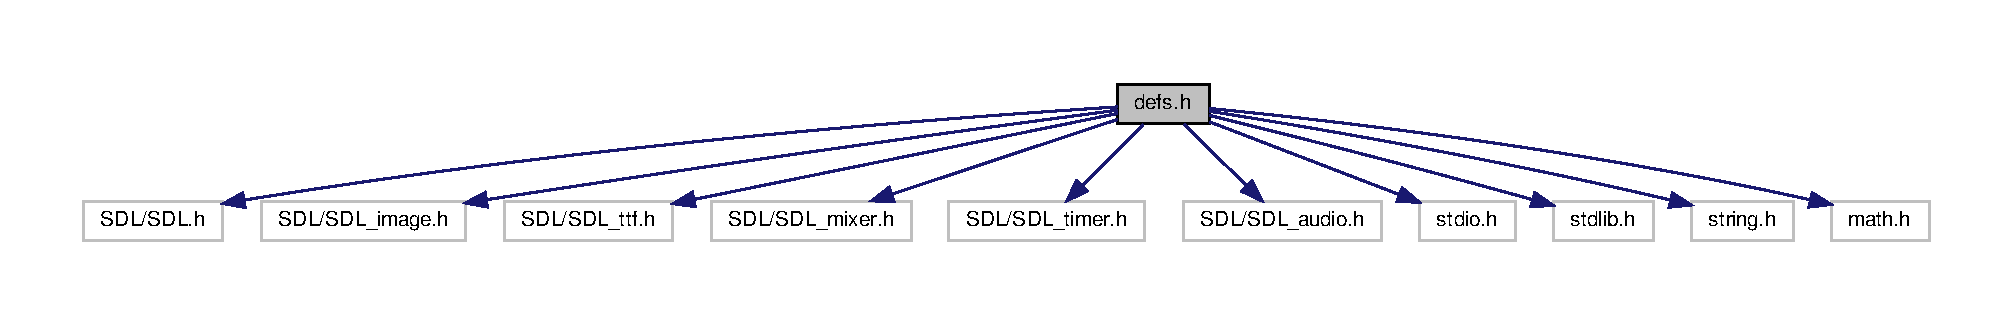
\includegraphics[width=350pt]{defs_8h__incl}
\end{center}
\end{figure}
This graph shows which files directly or indirectly include this file\+:
\nopagebreak
\begin{figure}[H]
\begin{center}
\leavevmode
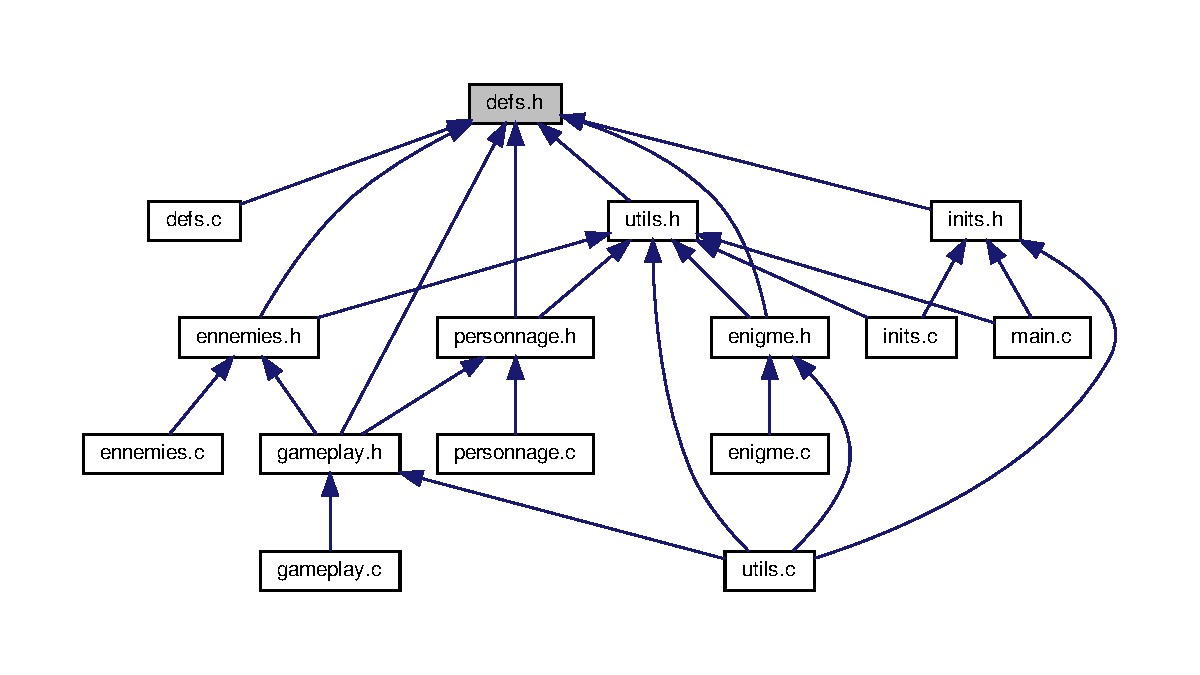
\includegraphics[width=350pt]{defs_8h__dep__incl}
\end{center}
\end{figure}
\subsection*{Macros}
\begin{DoxyCompactItemize}
\item 
\#define \hyperlink{defs_8h_a2cd109632a6dcccaa80b43561b1ab700}{S\+C\+R\+E\+E\+N\+\_\+\+W\+I\+D\+TH}~960
\item 
\#define \hyperlink{defs_8h_a6974d08a74da681b3957b2fead2608b8}{S\+C\+R\+E\+E\+N\+\_\+\+H\+E\+I\+G\+HT}~720
\item 
\#define \hyperlink{defs_8h_aeb696ed3736a3c9f76e7fd8193d3966f}{S\+C\+R\+E\+E\+N\+\_\+\+B\+PP}~32
\item 
\#define \hyperlink{defs_8h_a44dd1b46a3f55007e78fc1ac506153b9}{M\+A\+I\+N\+\_\+\+M\+E\+NU}~0
\item 
\#define \hyperlink{defs_8h_aa2d5c758628dddfa26e73ca5a245222a}{S\+E\+T\+T\+I\+N\+GS}~1
\item 
\#define \hyperlink{defs_8h_a4e58380df1435929cc191b5b4ba99cd5}{M\+AP}~2
\item 
\#define \hyperlink{defs_8h_a5e9640caa69c07b36781350d230585dc}{L\+E\+V\+E\+L1}~3
\item 
\#define \hyperlink{defs_8h_af03882265163ca6bf97fe86f8fac9044}{L\+E\+V\+E\+L2}~4
\item 
\#define \hyperlink{defs_8h_a4069806736a5968f80274abd9214c9bb}{L\+E\+V\+E\+L3}~5
\item 
\#define \hyperlink{defs_8h_ab870bbdbfa3927990efc5233a8a33cc8}{L\+E\+V\+E\+L4}~6
\item 
\#define \hyperlink{defs_8h_acaa9ceeac103b17d7dc460f452f1ef72}{E\+N\+I\+G\+M\+E\+D\+YN}~7
\item 
\#define \hyperlink{defs_8h_a1b55435b034bec164a03e10ca084fcd1}{E\+N\+I\+G\+M\+E\+S\+T\+A\+T\+I\+Q\+UE}~8
\item 
\#define \hyperlink{defs_8h_a04d46f28d25d5b97d577aa8ddc949fee}{M\+E\+N\+U\+\_\+\+F\+O\+NT}~\char`\"{}assets/ttf/B\+M\+Y\+E\+O\+N\+S\+U\+N\+G\+\_\+ttf.\+ttf\char`\"{}
\item 
\#define \hyperlink{defs_8h_a2c8adb01b1e2d9294c08c5adfd509c3f}{M\+E\+N\+U\+\_\+\+P\+O\+S\+\_\+W}~(\hyperlink{defs_8h_a2cd109632a6dcccaa80b43561b1ab700}{S\+C\+R\+E\+E\+N\+\_\+\+W\+I\+D\+TH} -\/ \hyperlink{defs_8h_a0c458e8109c971846c50a2a1e467bdb8}{menu\+Background}-\/$>$w) / 2
\item 
\#define \hyperlink{defs_8h_a367ad387284b353e953213d9f195af8a}{M\+E\+N\+U\+\_\+\+P\+O\+S\+\_\+H}~(\hyperlink{defs_8h_a6974d08a74da681b3957b2fead2608b8}{S\+C\+R\+E\+E\+N\+\_\+\+H\+E\+I\+G\+HT} -\/ \hyperlink{defs_8h_a0c458e8109c971846c50a2a1e467bdb8}{menu\+Background}-\/$>$h) / 2
\item 
\#define \hyperlink{defs_8h_a9cd0f9b6700aa0e8e19aa27d11a24d55}{I\+N\+F\+O\+\_\+\+P\+O\+S\+\_\+W}~((\hyperlink{defs_8h_a2cd109632a6dcccaa80b43561b1ab700}{S\+C\+R\+E\+E\+N\+\_\+\+W\+I\+D\+TH} -\/ \hyperlink{defs_8h_a29357cdf723f9f1d688a89fc9297c5df}{info\+Bar}-\/$>$w) / 2)
\item 
\#define \hyperlink{defs_8h_a4af857d907a5f61df35234948f166693}{I\+N\+F\+O\+\_\+\+P\+O\+S\+\_\+H}~((\hyperlink{defs_8h_a6974d08a74da681b3957b2fead2608b8}{S\+C\+R\+E\+E\+N\+\_\+\+H\+E\+I\+G\+HT} -\/ \hyperlink{defs_8h_a0c458e8109c971846c50a2a1e467bdb8}{menu\+Background}-\/$>$h) / 2) -\/ (int)(\hyperlink{defs_8h_a29357cdf723f9f1d688a89fc9297c5df}{info\+Bar}-\/$>$h / 2 $\ast$ 0.\+5)
\end{DoxyCompactItemize}
\subsection*{Typedefs}
\begin{DoxyCompactItemize}
\item 
typedef int \hyperlink{defs_8h_abf38e439d63c2001b8bbb96dbab1bd86}{State}
\end{DoxyCompactItemize}
\subsection*{Variables}
\begin{DoxyCompactItemize}
\item 
S\+D\+L\+\_\+\+Surface $\ast$ \hyperlink{defs_8h_a8a0695f3eaccf4eec9186f32ec831f20}{hello}
\item 
S\+D\+L\+\_\+\+Surface $\ast$ \hyperlink{defs_8h_a78ab7f4978e38e13edc4a80caf138817}{message}
\item 
S\+D\+L\+\_\+\+Surface $\ast$ \hyperlink{defs_8h_aa73601f944838ffac2fa4d3e298a6ef4}{image}
\item 
S\+D\+L\+\_\+\+Event \hyperlink{defs_8h_a6b57f01d3c576db5368dd0efc2f435a4}{event}
\item 
T\+T\+F\+\_\+\+Font $\ast$ \hyperlink{defs_8h_abf5bfa705e66ffc1ddaa6ce46c960873}{font}
\item 
S\+D\+L\+\_\+\+Color \hyperlink{defs_8h_a631bf4babe4c1825a2cdc0c19c2bd04f}{color}
\item 
S\+D\+L\+\_\+\+Surface \hyperlink{defs_8h_ac4c2a6228bd5522d3d403763262b9a22}{rect}
\item 
S\+D\+L\+\_\+\+Surface $\ast$ \hyperlink{defs_8h_ad22b3675c08f804b780be12b3d483c5f}{menu1}
\item 
S\+D\+L\+\_\+\+Surface $\ast$ \hyperlink{defs_8h_a417af12e04f849503ec50a1099905643}{menu2}
\item 
S\+D\+L\+\_\+\+Surface $\ast$ \hyperlink{defs_8h_a383dfb93f909d01760862403062962cc}{menu3}
\item 
S\+D\+L\+\_\+\+Surface $\ast$ \hyperlink{defs_8h_a18c72f024a1ea52461c5bdb3de91160b}{menu1\+Hover}
\item 
S\+D\+L\+\_\+\+Surface $\ast$ \hyperlink{defs_8h_ac61087fdd9269af636cd1bbfe69f66f0}{menu2\+Hover}
\item 
S\+D\+L\+\_\+\+Surface $\ast$ \hyperlink{defs_8h_ad0ae66eca85729f4a116652267974f1e}{menu3\+Hover}
\item 
S\+D\+L\+\_\+\+Surface $\ast$ \hyperlink{defs_8h_a0c458e8109c971846c50a2a1e467bdb8}{menu\+Background}
\item 
S\+D\+L\+\_\+\+Surface $\ast$ \hyperlink{defs_8h_acb8cf8a5a0ecc8929eb27322a5915fe0}{menu\+Button\+Normal\+State}
\item 
S\+D\+L\+\_\+\+Surface $\ast$ \hyperlink{defs_8h_a5f92b0799599a11b310d0446efb34eed}{menu\+Button\+Clicked\+State}
\item 
S\+D\+L\+\_\+\+Surface $\ast$ \hyperlink{defs_8h_a29357cdf723f9f1d688a89fc9297c5df}{info\+Bar}
\item 
S\+D\+L\+\_\+\+Surface $\ast$ \hyperlink{defs_8h_af40d2934209209a2bbdfc52395907442}{slider}
\item 
S\+D\+L\+\_\+\+Surface $\ast$ \hyperlink{defs_8h_a5026584637c9ab6c7453b6d06e7a8865}{slider\+Bar}
\item 
S\+D\+L\+\_\+\+Color \hyperlink{defs_8h_a355224f147f9e7c339a0b8758b349e12}{selected}
\item 
S\+D\+L\+\_\+\+Color \hyperlink{defs_8h_aa22a61780b279c453d06c92453d0fcf6}{n\+\_\+selected}
\item 
S\+D\+L\+\_\+\+Surface $\ast$ \hyperlink{defs_8h_aa345627708064725e35e666a540c6c91}{volume\+Bar}
\item 
S\+D\+L\+\_\+\+Surface $\ast$ \hyperlink{defs_8h_a89a3c2e9ba42e8d59258ecb6888d939f}{volume\+Selector}
\item 
int \hyperlink{defs_8h_a77bd4f876bdc3afed5acdd936f775d34}{seconds}
\item 
\hyperlink{defs_8h_abf38e439d63c2001b8bbb96dbab1bd86}{State} \hyperlink{defs_8h_a876b486d3a5241a126bd5751c5f70f79}{state}
\item 
int \hyperlink{defs_8h_a319f148f98ab6e78d52e318f4ce0c4f7}{fx\+Volume}
\item 
int \hyperlink{defs_8h_a93072262778c750b1245b6a70298ceeb}{music\+Volume}
\item 
int \hyperlink{defs_8h_adc359d0ba0a207e69da999c40bf762c8}{fullscreen}
\item 
S\+D\+L\+\_\+\+Surface $\ast$ \hyperlink{defs_8h_a603a0f6fe738992cfe8f14c4360a0e4e}{buttons}
\item 
Mix\+\_\+\+Music $\ast$ \hyperlink{defs_8h_ab203ceba3699c997bf63f13bbc33b33a}{music}
\item 
int \hyperlink{defs_8h_a85ea1b63086b31a15d3ed2579c5715a6}{mouseX}
\item 
int \hyperlink{defs_8h_a3637abebcaa9d04aa18b1610d0921e16}{mouseY}
\item 
int \hyperlink{defs_8h_a2d4592ccdd56a3f524dc0a6f1ac2e10c}{play\+State}
\item 
S\+D\+L\+\_\+\+Surface $\ast$ \hyperlink{defs_8h_a886ac8c83a9dd60d8ce8ea56b75237eb}{volume\+Surface}
\item 
S\+D\+L\+\_\+\+Surface $\ast$ \hyperlink{defs_8h_ae04cc1d68ad94e4a3b9b86bed1e6bff5}{window\+State}
\item 
char \hyperlink{defs_8h_ad1b99a8251e9e08198dd7d58712559d1}{window\+State\+Char} \mbox{[}15\mbox{]}
\item 
int \hyperlink{defs_8h_a27ed86ba911d1fc92308b64374dff8d6}{fullscreen\+Width}
\item 
int \hyperlink{defs_8h_a1f4b1ad6932d7a03cfba053932dce53b}{fullscreen\+Height}
\item 
S\+D\+L\+\_\+\+Surface $\ast$ \hyperlink{defs_8h_a0ac209296e33ac5089c4a4a5d3ee4b71}{new\+Game\+Button}
\item 
S\+D\+L\+\_\+\+Surface $\ast$ \hyperlink{defs_8h_ace1af332d79a0b6a47e8c597c1028776}{settings\+Button}
\item 
S\+D\+L\+\_\+\+Surface $\ast$ \hyperlink{defs_8h_a69599d632161dfcb6f030e1db3d8eed5}{quit\+Button}
\item 
S\+D\+L\+\_\+\+Surface $\ast$ \hyperlink{defs_8h_ad14ab720642740edf16e57f6c28ddbc9}{animation}
\item 
int \hyperlink{defs_8h_a45b3f1043a3b9217256cdb2129b7a0c4}{F\+PS}
\item 
int \hyperlink{defs_8h_ad30f972f2e6e3e5ecab0dee38ae6cdb8}{frame}
\item 
int \hyperlink{defs_8h_a2896431d6a80cd39b3d24b40237612ee}{quit}
\item 
int \hyperlink{defs_8h_a2c910ea1a2e2fd5d8b1bc80210ec26c1}{menu\+Select}
\item 
S\+D\+L\+\_\+\+Surface $\ast$ \hyperlink{defs_8h_a78fa3957d73de49cb81d047857504218}{screen}
\item 
S\+D\+L\+\_\+\+Surface $\ast$ \hyperlink{defs_8h_a68389876c2746622931d187c587f9c4d}{background}
\item 
Mix\+\_\+\+Chunk $\ast$ \hyperlink{defs_8h_a15b3213f20a453c753efb99f468778b7}{click}
\item 
Mix\+\_\+\+Chunk $\ast$ \hyperlink{defs_8h_af6976f3ff02b82755e3db73f9b3f93d9}{switcher}
\item 
Mix\+\_\+\+Chunk $\ast$ \hyperlink{defs_8h_a54c5edf6278e0284f9782bc30e46f21e}{fullscreen\+Sound}
\item 
int \hyperlink{defs_8h_ab5fd9003c5db26855fcce82ddc169de3}{settings\+State}
\item 
int \hyperlink{defs_8h_ac55d1466a0e202c7abb8ef4c1b1a0a23}{volume\+Slider}
\item 
S\+D\+L\+\_\+\+Surface $\ast$ \hyperlink{defs_8h_a0e03c4cc167dd7497007f1f3c8428f8a}{text1}
\item 
S\+D\+L\+\_\+\+Surface $\ast$ \hyperlink{defs_8h_acca77e0d07ce5db9ee27d900edf2bc93}{text2}
\item 
S\+D\+L\+\_\+\+Surface $\ast$ \hyperlink{defs_8h_af40006e8d3fb763f7ec6cc74a9d83f5d}{text3}
\item 
S\+D\+L\+\_\+\+Surface $\ast$ \hyperlink{defs_8h_abf63c96eaa5561e71eb0449c2485bc2d}{settings\+Text}
\item 
S\+D\+L\+\_\+\+Surface $\ast$ \hyperlink{defs_8h_ad9406ab79432c083dcb1957c8e5cda1d}{mode\+Text}
\item 
S\+D\+L\+\_\+\+Surface $\ast$ \hyperlink{defs_8h_a2daf8dd43d6c903576b69a36f87c634e}{full\+Screen\+Text}
\item 
S\+D\+L\+\_\+\+Surface $\ast$ \hyperlink{defs_8h_a89e33cac9585c151579a15753d98d5c9}{windowed\+Text}
\item 
S\+D\+L\+\_\+\+Surface $\ast$ \hyperlink{defs_8h_a5fed5a0a1d1c7bc2e6affebfb59fe08d}{volume\+Text}
\item 
S\+D\+L\+\_\+\+Surface $\ast$ \hyperlink{defs_8h_ad2f52297bb83f45d2b276e17c22ad26d}{exit\+Text}
\item 
int \hyperlink{defs_8h_af9af62c53df614f4a9b08e76938d340f}{key\+Pressed}
\item 
Uint32 \hyperlink{defs_8h_a0822b2f34b0cd24fc0a18aa2a73ee771}{next\+\_\+time}
\item 
int \hyperlink{defs_8h_a0ebc172bfb7854a6d992f3ee7636ec9b}{inits}
\item 
S\+D\+L\+\_\+\+Surface $\ast$ \hyperlink{defs_8h_a9dad4b780f049b0805f1000ebc312d8e}{game\+Background}
\item 
S\+D\+L\+\_\+\+Surface $\ast$ \hyperlink{defs_8h_a0ad344d281689f5b9f026a32af35a3d2}{game\+Background\+Mask}
\item 
int \hyperlink{defs_8h_ac68cd86607699f547cfa3ba4b3a4dfe5}{offset\+BG}
\item 
int \hyperlink{defs_8h_aef160b7437d94056f1dc59646cd5b87d}{score}
\item 
int \hyperlink{defs_8h_a7a0ba9e8c59a789d927afb3d70583403}{vies}
\item 
S\+D\+L\+\_\+\+Surface $\ast$ \hyperlink{defs_8h_a6c3f982896f92b962f6f61f17df23e52}{enigme\+Temp\+Image}
\item 
int \hyperlink{defs_8h_a27253d4a774a08a221ce3ddc7aab2ef5}{gameplay\+Start\+Tick}
\end{DoxyCompactItemize}


\subsection{Detailed Description}
global variables definitions 

\begin{DoxyAuthor}{Author}
Creative Sparks 
\end{DoxyAuthor}
\begin{DoxyVersion}{Version}
2.\+0 
\end{DoxyVersion}
\begin{DoxyDate}{Date}
2020 
\end{DoxyDate}


\subsection{Macro Definition Documentation}
\mbox{\Hypertarget{defs_8h_acaa9ceeac103b17d7dc460f452f1ef72}\label{defs_8h_acaa9ceeac103b17d7dc460f452f1ef72}} 
\index{defs.\+h@{defs.\+h}!E\+N\+I\+G\+M\+E\+D\+YN@{E\+N\+I\+G\+M\+E\+D\+YN}}
\index{E\+N\+I\+G\+M\+E\+D\+YN@{E\+N\+I\+G\+M\+E\+D\+YN}!defs.\+h@{defs.\+h}}
\subsubsection{\texorpdfstring{E\+N\+I\+G\+M\+E\+D\+YN}{ENIGMEDYN}}
{\footnotesize\ttfamily \#define E\+N\+I\+G\+M\+E\+D\+YN~7}

\mbox{\Hypertarget{defs_8h_a1b55435b034bec164a03e10ca084fcd1}\label{defs_8h_a1b55435b034bec164a03e10ca084fcd1}} 
\index{defs.\+h@{defs.\+h}!E\+N\+I\+G\+M\+E\+S\+T\+A\+T\+I\+Q\+UE@{E\+N\+I\+G\+M\+E\+S\+T\+A\+T\+I\+Q\+UE}}
\index{E\+N\+I\+G\+M\+E\+S\+T\+A\+T\+I\+Q\+UE@{E\+N\+I\+G\+M\+E\+S\+T\+A\+T\+I\+Q\+UE}!defs.\+h@{defs.\+h}}
\subsubsection{\texorpdfstring{E\+N\+I\+G\+M\+E\+S\+T\+A\+T\+I\+Q\+UE}{ENIGMESTATIQUE}}
{\footnotesize\ttfamily \#define E\+N\+I\+G\+M\+E\+S\+T\+A\+T\+I\+Q\+UE~8}

\mbox{\Hypertarget{defs_8h_a4af857d907a5f61df35234948f166693}\label{defs_8h_a4af857d907a5f61df35234948f166693}} 
\index{defs.\+h@{defs.\+h}!I\+N\+F\+O\+\_\+\+P\+O\+S\+\_\+H@{I\+N\+F\+O\+\_\+\+P\+O\+S\+\_\+H}}
\index{I\+N\+F\+O\+\_\+\+P\+O\+S\+\_\+H@{I\+N\+F\+O\+\_\+\+P\+O\+S\+\_\+H}!defs.\+h@{defs.\+h}}
\subsubsection{\texorpdfstring{I\+N\+F\+O\+\_\+\+P\+O\+S\+\_\+H}{INFO\_POS\_H}}
{\footnotesize\ttfamily \#define I\+N\+F\+O\+\_\+\+P\+O\+S\+\_\+H~((\hyperlink{defs_8h_a6974d08a74da681b3957b2fead2608b8}{S\+C\+R\+E\+E\+N\+\_\+\+H\+E\+I\+G\+HT} -\/ \hyperlink{defs_8h_a0c458e8109c971846c50a2a1e467bdb8}{menu\+Background}-\/$>$h) / 2) -\/ (int)(\hyperlink{defs_8h_a29357cdf723f9f1d688a89fc9297c5df}{info\+Bar}-\/$>$h / 2 $\ast$ 0.\+5)}

\mbox{\Hypertarget{defs_8h_a9cd0f9b6700aa0e8e19aa27d11a24d55}\label{defs_8h_a9cd0f9b6700aa0e8e19aa27d11a24d55}} 
\index{defs.\+h@{defs.\+h}!I\+N\+F\+O\+\_\+\+P\+O\+S\+\_\+W@{I\+N\+F\+O\+\_\+\+P\+O\+S\+\_\+W}}
\index{I\+N\+F\+O\+\_\+\+P\+O\+S\+\_\+W@{I\+N\+F\+O\+\_\+\+P\+O\+S\+\_\+W}!defs.\+h@{defs.\+h}}
\subsubsection{\texorpdfstring{I\+N\+F\+O\+\_\+\+P\+O\+S\+\_\+W}{INFO\_POS\_W}}
{\footnotesize\ttfamily \#define I\+N\+F\+O\+\_\+\+P\+O\+S\+\_\+W~((\hyperlink{defs_8h_a2cd109632a6dcccaa80b43561b1ab700}{S\+C\+R\+E\+E\+N\+\_\+\+W\+I\+D\+TH} -\/ \hyperlink{defs_8h_a29357cdf723f9f1d688a89fc9297c5df}{info\+Bar}-\/$>$w) / 2)}

\mbox{\Hypertarget{defs_8h_a5e9640caa69c07b36781350d230585dc}\label{defs_8h_a5e9640caa69c07b36781350d230585dc}} 
\index{defs.\+h@{defs.\+h}!L\+E\+V\+E\+L1@{L\+E\+V\+E\+L1}}
\index{L\+E\+V\+E\+L1@{L\+E\+V\+E\+L1}!defs.\+h@{defs.\+h}}
\subsubsection{\texorpdfstring{L\+E\+V\+E\+L1}{LEVEL1}}
{\footnotesize\ttfamily \#define L\+E\+V\+E\+L1~3}

\mbox{\Hypertarget{defs_8h_af03882265163ca6bf97fe86f8fac9044}\label{defs_8h_af03882265163ca6bf97fe86f8fac9044}} 
\index{defs.\+h@{defs.\+h}!L\+E\+V\+E\+L2@{L\+E\+V\+E\+L2}}
\index{L\+E\+V\+E\+L2@{L\+E\+V\+E\+L2}!defs.\+h@{defs.\+h}}
\subsubsection{\texorpdfstring{L\+E\+V\+E\+L2}{LEVEL2}}
{\footnotesize\ttfamily \#define L\+E\+V\+E\+L2~4}

\mbox{\Hypertarget{defs_8h_a4069806736a5968f80274abd9214c9bb}\label{defs_8h_a4069806736a5968f80274abd9214c9bb}} 
\index{defs.\+h@{defs.\+h}!L\+E\+V\+E\+L3@{L\+E\+V\+E\+L3}}
\index{L\+E\+V\+E\+L3@{L\+E\+V\+E\+L3}!defs.\+h@{defs.\+h}}
\subsubsection{\texorpdfstring{L\+E\+V\+E\+L3}{LEVEL3}}
{\footnotesize\ttfamily \#define L\+E\+V\+E\+L3~5}

\mbox{\Hypertarget{defs_8h_ab870bbdbfa3927990efc5233a8a33cc8}\label{defs_8h_ab870bbdbfa3927990efc5233a8a33cc8}} 
\index{defs.\+h@{defs.\+h}!L\+E\+V\+E\+L4@{L\+E\+V\+E\+L4}}
\index{L\+E\+V\+E\+L4@{L\+E\+V\+E\+L4}!defs.\+h@{defs.\+h}}
\subsubsection{\texorpdfstring{L\+E\+V\+E\+L4}{LEVEL4}}
{\footnotesize\ttfamily \#define L\+E\+V\+E\+L4~6}

\mbox{\Hypertarget{defs_8h_a44dd1b46a3f55007e78fc1ac506153b9}\label{defs_8h_a44dd1b46a3f55007e78fc1ac506153b9}} 
\index{defs.\+h@{defs.\+h}!M\+A\+I\+N\+\_\+\+M\+E\+NU@{M\+A\+I\+N\+\_\+\+M\+E\+NU}}
\index{M\+A\+I\+N\+\_\+\+M\+E\+NU@{M\+A\+I\+N\+\_\+\+M\+E\+NU}!defs.\+h@{defs.\+h}}
\subsubsection{\texorpdfstring{M\+A\+I\+N\+\_\+\+M\+E\+NU}{MAIN\_MENU}}
{\footnotesize\ttfamily \#define M\+A\+I\+N\+\_\+\+M\+E\+NU~0}

\mbox{\Hypertarget{defs_8h_a4e58380df1435929cc191b5b4ba99cd5}\label{defs_8h_a4e58380df1435929cc191b5b4ba99cd5}} 
\index{defs.\+h@{defs.\+h}!M\+AP@{M\+AP}}
\index{M\+AP@{M\+AP}!defs.\+h@{defs.\+h}}
\subsubsection{\texorpdfstring{M\+AP}{MAP}}
{\footnotesize\ttfamily \#define M\+AP~2}

\mbox{\Hypertarget{defs_8h_a04d46f28d25d5b97d577aa8ddc949fee}\label{defs_8h_a04d46f28d25d5b97d577aa8ddc949fee}} 
\index{defs.\+h@{defs.\+h}!M\+E\+N\+U\+\_\+\+F\+O\+NT@{M\+E\+N\+U\+\_\+\+F\+O\+NT}}
\index{M\+E\+N\+U\+\_\+\+F\+O\+NT@{M\+E\+N\+U\+\_\+\+F\+O\+NT}!defs.\+h@{defs.\+h}}
\subsubsection{\texorpdfstring{M\+E\+N\+U\+\_\+\+F\+O\+NT}{MENU\_FONT}}
{\footnotesize\ttfamily \#define M\+E\+N\+U\+\_\+\+F\+O\+NT~\char`\"{}assets/ttf/B\+M\+Y\+E\+O\+N\+S\+U\+N\+G\+\_\+ttf.\+ttf\char`\"{}}

\mbox{\Hypertarget{defs_8h_a367ad387284b353e953213d9f195af8a}\label{defs_8h_a367ad387284b353e953213d9f195af8a}} 
\index{defs.\+h@{defs.\+h}!M\+E\+N\+U\+\_\+\+P\+O\+S\+\_\+H@{M\+E\+N\+U\+\_\+\+P\+O\+S\+\_\+H}}
\index{M\+E\+N\+U\+\_\+\+P\+O\+S\+\_\+H@{M\+E\+N\+U\+\_\+\+P\+O\+S\+\_\+H}!defs.\+h@{defs.\+h}}
\subsubsection{\texorpdfstring{M\+E\+N\+U\+\_\+\+P\+O\+S\+\_\+H}{MENU\_POS\_H}}
{\footnotesize\ttfamily \#define M\+E\+N\+U\+\_\+\+P\+O\+S\+\_\+H~(\hyperlink{defs_8h_a6974d08a74da681b3957b2fead2608b8}{S\+C\+R\+E\+E\+N\+\_\+\+H\+E\+I\+G\+HT} -\/ \hyperlink{defs_8h_a0c458e8109c971846c50a2a1e467bdb8}{menu\+Background}-\/$>$h) / 2}

\mbox{\Hypertarget{defs_8h_a2c8adb01b1e2d9294c08c5adfd509c3f}\label{defs_8h_a2c8adb01b1e2d9294c08c5adfd509c3f}} 
\index{defs.\+h@{defs.\+h}!M\+E\+N\+U\+\_\+\+P\+O\+S\+\_\+W@{M\+E\+N\+U\+\_\+\+P\+O\+S\+\_\+W}}
\index{M\+E\+N\+U\+\_\+\+P\+O\+S\+\_\+W@{M\+E\+N\+U\+\_\+\+P\+O\+S\+\_\+W}!defs.\+h@{defs.\+h}}
\subsubsection{\texorpdfstring{M\+E\+N\+U\+\_\+\+P\+O\+S\+\_\+W}{MENU\_POS\_W}}
{\footnotesize\ttfamily \#define M\+E\+N\+U\+\_\+\+P\+O\+S\+\_\+W~(\hyperlink{defs_8h_a2cd109632a6dcccaa80b43561b1ab700}{S\+C\+R\+E\+E\+N\+\_\+\+W\+I\+D\+TH} -\/ \hyperlink{defs_8h_a0c458e8109c971846c50a2a1e467bdb8}{menu\+Background}-\/$>$w) / 2}

\mbox{\Hypertarget{defs_8h_aeb696ed3736a3c9f76e7fd8193d3966f}\label{defs_8h_aeb696ed3736a3c9f76e7fd8193d3966f}} 
\index{defs.\+h@{defs.\+h}!S\+C\+R\+E\+E\+N\+\_\+\+B\+PP@{S\+C\+R\+E\+E\+N\+\_\+\+B\+PP}}
\index{S\+C\+R\+E\+E\+N\+\_\+\+B\+PP@{S\+C\+R\+E\+E\+N\+\_\+\+B\+PP}!defs.\+h@{defs.\+h}}
\subsubsection{\texorpdfstring{S\+C\+R\+E\+E\+N\+\_\+\+B\+PP}{SCREEN\_BPP}}
{\footnotesize\ttfamily \#define S\+C\+R\+E\+E\+N\+\_\+\+B\+PP~32}

\mbox{\Hypertarget{defs_8h_a6974d08a74da681b3957b2fead2608b8}\label{defs_8h_a6974d08a74da681b3957b2fead2608b8}} 
\index{defs.\+h@{defs.\+h}!S\+C\+R\+E\+E\+N\+\_\+\+H\+E\+I\+G\+HT@{S\+C\+R\+E\+E\+N\+\_\+\+H\+E\+I\+G\+HT}}
\index{S\+C\+R\+E\+E\+N\+\_\+\+H\+E\+I\+G\+HT@{S\+C\+R\+E\+E\+N\+\_\+\+H\+E\+I\+G\+HT}!defs.\+h@{defs.\+h}}
\subsubsection{\texorpdfstring{S\+C\+R\+E\+E\+N\+\_\+\+H\+E\+I\+G\+HT}{SCREEN\_HEIGHT}}
{\footnotesize\ttfamily \#define S\+C\+R\+E\+E\+N\+\_\+\+H\+E\+I\+G\+HT~720}

\mbox{\Hypertarget{defs_8h_a2cd109632a6dcccaa80b43561b1ab700}\label{defs_8h_a2cd109632a6dcccaa80b43561b1ab700}} 
\index{defs.\+h@{defs.\+h}!S\+C\+R\+E\+E\+N\+\_\+\+W\+I\+D\+TH@{S\+C\+R\+E\+E\+N\+\_\+\+W\+I\+D\+TH}}
\index{S\+C\+R\+E\+E\+N\+\_\+\+W\+I\+D\+TH@{S\+C\+R\+E\+E\+N\+\_\+\+W\+I\+D\+TH}!defs.\+h@{defs.\+h}}
\subsubsection{\texorpdfstring{S\+C\+R\+E\+E\+N\+\_\+\+W\+I\+D\+TH}{SCREEN\_WIDTH}}
{\footnotesize\ttfamily \#define S\+C\+R\+E\+E\+N\+\_\+\+W\+I\+D\+TH~960}

\mbox{\Hypertarget{defs_8h_aa2d5c758628dddfa26e73ca5a245222a}\label{defs_8h_aa2d5c758628dddfa26e73ca5a245222a}} 
\index{defs.\+h@{defs.\+h}!S\+E\+T\+T\+I\+N\+GS@{S\+E\+T\+T\+I\+N\+GS}}
\index{S\+E\+T\+T\+I\+N\+GS@{S\+E\+T\+T\+I\+N\+GS}!defs.\+h@{defs.\+h}}
\subsubsection{\texorpdfstring{S\+E\+T\+T\+I\+N\+GS}{SETTINGS}}
{\footnotesize\ttfamily \#define S\+E\+T\+T\+I\+N\+GS~1}



\subsection{Typedef Documentation}
\mbox{\Hypertarget{defs_8h_abf38e439d63c2001b8bbb96dbab1bd86}\label{defs_8h_abf38e439d63c2001b8bbb96dbab1bd86}} 
\index{defs.\+h@{defs.\+h}!State@{State}}
\index{State@{State}!defs.\+h@{defs.\+h}}
\subsubsection{\texorpdfstring{State}{State}}
{\footnotesize\ttfamily typedef int \hyperlink{defs_8h_abf38e439d63c2001b8bbb96dbab1bd86}{State}}



\subsection{Variable Documentation}
\mbox{\Hypertarget{defs_8h_ad14ab720642740edf16e57f6c28ddbc9}\label{defs_8h_ad14ab720642740edf16e57f6c28ddbc9}} 
\index{defs.\+h@{defs.\+h}!animation@{animation}}
\index{animation@{animation}!defs.\+h@{defs.\+h}}
\subsubsection{\texorpdfstring{animation}{animation}}
{\footnotesize\ttfamily S\+D\+L\+\_\+\+Surface$\ast$ animation}

\mbox{\Hypertarget{defs_8h_a68389876c2746622931d187c587f9c4d}\label{defs_8h_a68389876c2746622931d187c587f9c4d}} 
\index{defs.\+h@{defs.\+h}!background@{background}}
\index{background@{background}!defs.\+h@{defs.\+h}}
\subsubsection{\texorpdfstring{background}{background}}
{\footnotesize\ttfamily S\+D\+L\+\_\+\+Surface$\ast$ background}

\mbox{\Hypertarget{defs_8h_a603a0f6fe738992cfe8f14c4360a0e4e}\label{defs_8h_a603a0f6fe738992cfe8f14c4360a0e4e}} 
\index{defs.\+h@{defs.\+h}!buttons@{buttons}}
\index{buttons@{buttons}!defs.\+h@{defs.\+h}}
\subsubsection{\texorpdfstring{buttons}{buttons}}
{\footnotesize\ttfamily S\+D\+L\+\_\+\+Surface$\ast$ buttons}

\mbox{\Hypertarget{defs_8h_a15b3213f20a453c753efb99f468778b7}\label{defs_8h_a15b3213f20a453c753efb99f468778b7}} 
\index{defs.\+h@{defs.\+h}!click@{click}}
\index{click@{click}!defs.\+h@{defs.\+h}}
\subsubsection{\texorpdfstring{click}{click}}
{\footnotesize\ttfamily Mix\+\_\+\+Chunk$\ast$ click}

\mbox{\Hypertarget{defs_8h_a631bf4babe4c1825a2cdc0c19c2bd04f}\label{defs_8h_a631bf4babe4c1825a2cdc0c19c2bd04f}} 
\index{defs.\+h@{defs.\+h}!color@{color}}
\index{color@{color}!defs.\+h@{defs.\+h}}
\subsubsection{\texorpdfstring{color}{color}}
{\footnotesize\ttfamily S\+D\+L\+\_\+\+Color color}

\mbox{\Hypertarget{defs_8h_a6c3f982896f92b962f6f61f17df23e52}\label{defs_8h_a6c3f982896f92b962f6f61f17df23e52}} 
\index{defs.\+h@{defs.\+h}!enigme\+Temp\+Image@{enigme\+Temp\+Image}}
\index{enigme\+Temp\+Image@{enigme\+Temp\+Image}!defs.\+h@{defs.\+h}}
\subsubsection{\texorpdfstring{enigme\+Temp\+Image}{enigmeTempImage}}
{\footnotesize\ttfamily S\+D\+L\+\_\+\+Surface$\ast$ enigme\+Temp\+Image}

\mbox{\Hypertarget{defs_8h_a6b57f01d3c576db5368dd0efc2f435a4}\label{defs_8h_a6b57f01d3c576db5368dd0efc2f435a4}} 
\index{defs.\+h@{defs.\+h}!event@{event}}
\index{event@{event}!defs.\+h@{defs.\+h}}
\subsubsection{\texorpdfstring{event}{event}}
{\footnotesize\ttfamily S\+D\+L\+\_\+\+Event event}

\mbox{\Hypertarget{defs_8h_ad2f52297bb83f45d2b276e17c22ad26d}\label{defs_8h_ad2f52297bb83f45d2b276e17c22ad26d}} 
\index{defs.\+h@{defs.\+h}!exit\+Text@{exit\+Text}}
\index{exit\+Text@{exit\+Text}!defs.\+h@{defs.\+h}}
\subsubsection{\texorpdfstring{exit\+Text}{exitText}}
{\footnotesize\ttfamily S\+D\+L\+\_\+\+Surface$\ast$ exit\+Text}

\mbox{\Hypertarget{defs_8h_abf5bfa705e66ffc1ddaa6ce46c960873}\label{defs_8h_abf5bfa705e66ffc1ddaa6ce46c960873}} 
\index{defs.\+h@{defs.\+h}!font@{font}}
\index{font@{font}!defs.\+h@{defs.\+h}}
\subsubsection{\texorpdfstring{font}{font}}
{\footnotesize\ttfamily T\+T\+F\+\_\+\+Font$\ast$ font}

\mbox{\Hypertarget{defs_8h_a45b3f1043a3b9217256cdb2129b7a0c4}\label{defs_8h_a45b3f1043a3b9217256cdb2129b7a0c4}} 
\index{defs.\+h@{defs.\+h}!F\+PS@{F\+PS}}
\index{F\+PS@{F\+PS}!defs.\+h@{defs.\+h}}
\subsubsection{\texorpdfstring{F\+PS}{FPS}}
{\footnotesize\ttfamily int F\+PS}

\mbox{\Hypertarget{defs_8h_ad30f972f2e6e3e5ecab0dee38ae6cdb8}\label{defs_8h_ad30f972f2e6e3e5ecab0dee38ae6cdb8}} 
\index{defs.\+h@{defs.\+h}!frame@{frame}}
\index{frame@{frame}!defs.\+h@{defs.\+h}}
\subsubsection{\texorpdfstring{frame}{frame}}
{\footnotesize\ttfamily int frame}

\mbox{\Hypertarget{defs_8h_adc359d0ba0a207e69da999c40bf762c8}\label{defs_8h_adc359d0ba0a207e69da999c40bf762c8}} 
\index{defs.\+h@{defs.\+h}!fullscreen@{fullscreen}}
\index{fullscreen@{fullscreen}!defs.\+h@{defs.\+h}}
\subsubsection{\texorpdfstring{fullscreen}{fullscreen}}
{\footnotesize\ttfamily int fullscreen}

\mbox{\Hypertarget{defs_8h_a1f4b1ad6932d7a03cfba053932dce53b}\label{defs_8h_a1f4b1ad6932d7a03cfba053932dce53b}} 
\index{defs.\+h@{defs.\+h}!fullscreen\+Height@{fullscreen\+Height}}
\index{fullscreen\+Height@{fullscreen\+Height}!defs.\+h@{defs.\+h}}
\subsubsection{\texorpdfstring{fullscreen\+Height}{fullscreenHeight}}
{\footnotesize\ttfamily int fullscreen\+Height}

\mbox{\Hypertarget{defs_8h_a54c5edf6278e0284f9782bc30e46f21e}\label{defs_8h_a54c5edf6278e0284f9782bc30e46f21e}} 
\index{defs.\+h@{defs.\+h}!fullscreen\+Sound@{fullscreen\+Sound}}
\index{fullscreen\+Sound@{fullscreen\+Sound}!defs.\+h@{defs.\+h}}
\subsubsection{\texorpdfstring{fullscreen\+Sound}{fullscreenSound}}
{\footnotesize\ttfamily Mix\+\_\+\+Chunk$\ast$ fullscreen\+Sound}

\mbox{\Hypertarget{defs_8h_a2daf8dd43d6c903576b69a36f87c634e}\label{defs_8h_a2daf8dd43d6c903576b69a36f87c634e}} 
\index{defs.\+h@{defs.\+h}!full\+Screen\+Text@{full\+Screen\+Text}}
\index{full\+Screen\+Text@{full\+Screen\+Text}!defs.\+h@{defs.\+h}}
\subsubsection{\texorpdfstring{full\+Screen\+Text}{fullScreenText}}
{\footnotesize\ttfamily S\+D\+L\+\_\+\+Surface$\ast$ full\+Screen\+Text}

\mbox{\Hypertarget{defs_8h_a27ed86ba911d1fc92308b64374dff8d6}\label{defs_8h_a27ed86ba911d1fc92308b64374dff8d6}} 
\index{defs.\+h@{defs.\+h}!fullscreen\+Width@{fullscreen\+Width}}
\index{fullscreen\+Width@{fullscreen\+Width}!defs.\+h@{defs.\+h}}
\subsubsection{\texorpdfstring{fullscreen\+Width}{fullscreenWidth}}
{\footnotesize\ttfamily int fullscreen\+Width}

\mbox{\Hypertarget{defs_8h_a319f148f98ab6e78d52e318f4ce0c4f7}\label{defs_8h_a319f148f98ab6e78d52e318f4ce0c4f7}} 
\index{defs.\+h@{defs.\+h}!fx\+Volume@{fx\+Volume}}
\index{fx\+Volume@{fx\+Volume}!defs.\+h@{defs.\+h}}
\subsubsection{\texorpdfstring{fx\+Volume}{fxVolume}}
{\footnotesize\ttfamily int fx\+Volume}

\mbox{\Hypertarget{defs_8h_a9dad4b780f049b0805f1000ebc312d8e}\label{defs_8h_a9dad4b780f049b0805f1000ebc312d8e}} 
\index{defs.\+h@{defs.\+h}!game\+Background@{game\+Background}}
\index{game\+Background@{game\+Background}!defs.\+h@{defs.\+h}}
\subsubsection{\texorpdfstring{game\+Background}{gameBackground}}
{\footnotesize\ttfamily S\+D\+L\+\_\+\+Surface$\ast$ game\+Background}

\mbox{\Hypertarget{defs_8h_a0ad344d281689f5b9f026a32af35a3d2}\label{defs_8h_a0ad344d281689f5b9f026a32af35a3d2}} 
\index{defs.\+h@{defs.\+h}!game\+Background\+Mask@{game\+Background\+Mask}}
\index{game\+Background\+Mask@{game\+Background\+Mask}!defs.\+h@{defs.\+h}}
\subsubsection{\texorpdfstring{game\+Background\+Mask}{gameBackgroundMask}}
{\footnotesize\ttfamily S\+D\+L\+\_\+\+Surface$\ast$ game\+Background\+Mask}

\mbox{\Hypertarget{defs_8h_a27253d4a774a08a221ce3ddc7aab2ef5}\label{defs_8h_a27253d4a774a08a221ce3ddc7aab2ef5}} 
\index{defs.\+h@{defs.\+h}!gameplay\+Start\+Tick@{gameplay\+Start\+Tick}}
\index{gameplay\+Start\+Tick@{gameplay\+Start\+Tick}!defs.\+h@{defs.\+h}}
\subsubsection{\texorpdfstring{gameplay\+Start\+Tick}{gameplayStartTick}}
{\footnotesize\ttfamily int gameplay\+Start\+Tick}

\mbox{\Hypertarget{defs_8h_a8a0695f3eaccf4eec9186f32ec831f20}\label{defs_8h_a8a0695f3eaccf4eec9186f32ec831f20}} 
\index{defs.\+h@{defs.\+h}!hello@{hello}}
\index{hello@{hello}!defs.\+h@{defs.\+h}}
\subsubsection{\texorpdfstring{hello}{hello}}
{\footnotesize\ttfamily S\+D\+L\+\_\+\+Surface$\ast$ hello}

\mbox{\Hypertarget{defs_8h_aa73601f944838ffac2fa4d3e298a6ef4}\label{defs_8h_aa73601f944838ffac2fa4d3e298a6ef4}} 
\index{defs.\+h@{defs.\+h}!image@{image}}
\index{image@{image}!defs.\+h@{defs.\+h}}
\subsubsection{\texorpdfstring{image}{image}}
{\footnotesize\ttfamily S\+D\+L\+\_\+\+Surface$\ast$ image}

\mbox{\Hypertarget{defs_8h_a29357cdf723f9f1d688a89fc9297c5df}\label{defs_8h_a29357cdf723f9f1d688a89fc9297c5df}} 
\index{defs.\+h@{defs.\+h}!info\+Bar@{info\+Bar}}
\index{info\+Bar@{info\+Bar}!defs.\+h@{defs.\+h}}
\subsubsection{\texorpdfstring{info\+Bar}{infoBar}}
{\footnotesize\ttfamily S\+D\+L\+\_\+\+Surface$\ast$ info\+Bar}

\mbox{\Hypertarget{defs_8h_a0ebc172bfb7854a6d992f3ee7636ec9b}\label{defs_8h_a0ebc172bfb7854a6d992f3ee7636ec9b}} 
\index{defs.\+h@{defs.\+h}!inits@{inits}}
\index{inits@{inits}!defs.\+h@{defs.\+h}}
\subsubsection{\texorpdfstring{inits}{inits}}
{\footnotesize\ttfamily int inits}

\mbox{\Hypertarget{defs_8h_af9af62c53df614f4a9b08e76938d340f}\label{defs_8h_af9af62c53df614f4a9b08e76938d340f}} 
\index{defs.\+h@{defs.\+h}!key\+Pressed@{key\+Pressed}}
\index{key\+Pressed@{key\+Pressed}!defs.\+h@{defs.\+h}}
\subsubsection{\texorpdfstring{key\+Pressed}{keyPressed}}
{\footnotesize\ttfamily int key\+Pressed}

\mbox{\Hypertarget{defs_8h_ad22b3675c08f804b780be12b3d483c5f}\label{defs_8h_ad22b3675c08f804b780be12b3d483c5f}} 
\index{defs.\+h@{defs.\+h}!menu1@{menu1}}
\index{menu1@{menu1}!defs.\+h@{defs.\+h}}
\subsubsection{\texorpdfstring{menu1}{menu1}}
{\footnotesize\ttfamily S\+D\+L\+\_\+\+Surface$\ast$ menu1}

\mbox{\Hypertarget{defs_8h_a18c72f024a1ea52461c5bdb3de91160b}\label{defs_8h_a18c72f024a1ea52461c5bdb3de91160b}} 
\index{defs.\+h@{defs.\+h}!menu1\+Hover@{menu1\+Hover}}
\index{menu1\+Hover@{menu1\+Hover}!defs.\+h@{defs.\+h}}
\subsubsection{\texorpdfstring{menu1\+Hover}{menu1Hover}}
{\footnotesize\ttfamily S\+D\+L\+\_\+\+Surface$\ast$ menu1\+Hover}

\mbox{\Hypertarget{defs_8h_a417af12e04f849503ec50a1099905643}\label{defs_8h_a417af12e04f849503ec50a1099905643}} 
\index{defs.\+h@{defs.\+h}!menu2@{menu2}}
\index{menu2@{menu2}!defs.\+h@{defs.\+h}}
\subsubsection{\texorpdfstring{menu2}{menu2}}
{\footnotesize\ttfamily S\+D\+L\+\_\+\+Surface$\ast$ menu2}

\mbox{\Hypertarget{defs_8h_ac61087fdd9269af636cd1bbfe69f66f0}\label{defs_8h_ac61087fdd9269af636cd1bbfe69f66f0}} 
\index{defs.\+h@{defs.\+h}!menu2\+Hover@{menu2\+Hover}}
\index{menu2\+Hover@{menu2\+Hover}!defs.\+h@{defs.\+h}}
\subsubsection{\texorpdfstring{menu2\+Hover}{menu2Hover}}
{\footnotesize\ttfamily S\+D\+L\+\_\+\+Surface$\ast$ menu2\+Hover}

\mbox{\Hypertarget{defs_8h_a383dfb93f909d01760862403062962cc}\label{defs_8h_a383dfb93f909d01760862403062962cc}} 
\index{defs.\+h@{defs.\+h}!menu3@{menu3}}
\index{menu3@{menu3}!defs.\+h@{defs.\+h}}
\subsubsection{\texorpdfstring{menu3}{menu3}}
{\footnotesize\ttfamily S\+D\+L\+\_\+\+Surface$\ast$ menu3}

\mbox{\Hypertarget{defs_8h_ad0ae66eca85729f4a116652267974f1e}\label{defs_8h_ad0ae66eca85729f4a116652267974f1e}} 
\index{defs.\+h@{defs.\+h}!menu3\+Hover@{menu3\+Hover}}
\index{menu3\+Hover@{menu3\+Hover}!defs.\+h@{defs.\+h}}
\subsubsection{\texorpdfstring{menu3\+Hover}{menu3Hover}}
{\footnotesize\ttfamily S\+D\+L\+\_\+\+Surface$\ast$ menu3\+Hover}

\mbox{\Hypertarget{defs_8h_a0c458e8109c971846c50a2a1e467bdb8}\label{defs_8h_a0c458e8109c971846c50a2a1e467bdb8}} 
\index{defs.\+h@{defs.\+h}!menu\+Background@{menu\+Background}}
\index{menu\+Background@{menu\+Background}!defs.\+h@{defs.\+h}}
\subsubsection{\texorpdfstring{menu\+Background}{menuBackground}}
{\footnotesize\ttfamily S\+D\+L\+\_\+\+Surface$\ast$ menu\+Background}

\mbox{\Hypertarget{defs_8h_a5f92b0799599a11b310d0446efb34eed}\label{defs_8h_a5f92b0799599a11b310d0446efb34eed}} 
\index{defs.\+h@{defs.\+h}!menu\+Button\+Clicked\+State@{menu\+Button\+Clicked\+State}}
\index{menu\+Button\+Clicked\+State@{menu\+Button\+Clicked\+State}!defs.\+h@{defs.\+h}}
\subsubsection{\texorpdfstring{menu\+Button\+Clicked\+State}{menuButtonClickedState}}
{\footnotesize\ttfamily S\+D\+L\+\_\+\+Surface$\ast$ menu\+Button\+Clicked\+State}

\mbox{\Hypertarget{defs_8h_acb8cf8a5a0ecc8929eb27322a5915fe0}\label{defs_8h_acb8cf8a5a0ecc8929eb27322a5915fe0}} 
\index{defs.\+h@{defs.\+h}!menu\+Button\+Normal\+State@{menu\+Button\+Normal\+State}}
\index{menu\+Button\+Normal\+State@{menu\+Button\+Normal\+State}!defs.\+h@{defs.\+h}}
\subsubsection{\texorpdfstring{menu\+Button\+Normal\+State}{menuButtonNormalState}}
{\footnotesize\ttfamily S\+D\+L\+\_\+\+Surface$\ast$ menu\+Button\+Normal\+State}

\mbox{\Hypertarget{defs_8h_a2c910ea1a2e2fd5d8b1bc80210ec26c1}\label{defs_8h_a2c910ea1a2e2fd5d8b1bc80210ec26c1}} 
\index{defs.\+h@{defs.\+h}!menu\+Select@{menu\+Select}}
\index{menu\+Select@{menu\+Select}!defs.\+h@{defs.\+h}}
\subsubsection{\texorpdfstring{menu\+Select}{menuSelect}}
{\footnotesize\ttfamily int menu\+Select}

\mbox{\Hypertarget{defs_8h_a78ab7f4978e38e13edc4a80caf138817}\label{defs_8h_a78ab7f4978e38e13edc4a80caf138817}} 
\index{defs.\+h@{defs.\+h}!message@{message}}
\index{message@{message}!defs.\+h@{defs.\+h}}
\subsubsection{\texorpdfstring{message}{message}}
{\footnotesize\ttfamily S\+D\+L\+\_\+\+Surface$\ast$ message}

\mbox{\Hypertarget{defs_8h_ad9406ab79432c083dcb1957c8e5cda1d}\label{defs_8h_ad9406ab79432c083dcb1957c8e5cda1d}} 
\index{defs.\+h@{defs.\+h}!mode\+Text@{mode\+Text}}
\index{mode\+Text@{mode\+Text}!defs.\+h@{defs.\+h}}
\subsubsection{\texorpdfstring{mode\+Text}{modeText}}
{\footnotesize\ttfamily S\+D\+L\+\_\+\+Surface$\ast$ mode\+Text}

\mbox{\Hypertarget{defs_8h_a85ea1b63086b31a15d3ed2579c5715a6}\label{defs_8h_a85ea1b63086b31a15d3ed2579c5715a6}} 
\index{defs.\+h@{defs.\+h}!mouseX@{mouseX}}
\index{mouseX@{mouseX}!defs.\+h@{defs.\+h}}
\subsubsection{\texorpdfstring{mouseX}{mouseX}}
{\footnotesize\ttfamily int mouseX}

\mbox{\Hypertarget{defs_8h_a3637abebcaa9d04aa18b1610d0921e16}\label{defs_8h_a3637abebcaa9d04aa18b1610d0921e16}} 
\index{defs.\+h@{defs.\+h}!mouseY@{mouseY}}
\index{mouseY@{mouseY}!defs.\+h@{defs.\+h}}
\subsubsection{\texorpdfstring{mouseY}{mouseY}}
{\footnotesize\ttfamily int mouseY}

\mbox{\Hypertarget{defs_8h_ab203ceba3699c997bf63f13bbc33b33a}\label{defs_8h_ab203ceba3699c997bf63f13bbc33b33a}} 
\index{defs.\+h@{defs.\+h}!music@{music}}
\index{music@{music}!defs.\+h@{defs.\+h}}
\subsubsection{\texorpdfstring{music}{music}}
{\footnotesize\ttfamily Mix\+\_\+\+Music$\ast$ music}

\mbox{\Hypertarget{defs_8h_a93072262778c750b1245b6a70298ceeb}\label{defs_8h_a93072262778c750b1245b6a70298ceeb}} 
\index{defs.\+h@{defs.\+h}!music\+Volume@{music\+Volume}}
\index{music\+Volume@{music\+Volume}!defs.\+h@{defs.\+h}}
\subsubsection{\texorpdfstring{music\+Volume}{musicVolume}}
{\footnotesize\ttfamily int music\+Volume}

\mbox{\Hypertarget{defs_8h_aa22a61780b279c453d06c92453d0fcf6}\label{defs_8h_aa22a61780b279c453d06c92453d0fcf6}} 
\index{defs.\+h@{defs.\+h}!n\+\_\+selected@{n\+\_\+selected}}
\index{n\+\_\+selected@{n\+\_\+selected}!defs.\+h@{defs.\+h}}
\subsubsection{\texorpdfstring{n\+\_\+selected}{n\_selected}}
{\footnotesize\ttfamily S\+D\+L\+\_\+\+Color n\+\_\+selected}

\mbox{\Hypertarget{defs_8h_a0ac209296e33ac5089c4a4a5d3ee4b71}\label{defs_8h_a0ac209296e33ac5089c4a4a5d3ee4b71}} 
\index{defs.\+h@{defs.\+h}!new\+Game\+Button@{new\+Game\+Button}}
\index{new\+Game\+Button@{new\+Game\+Button}!defs.\+h@{defs.\+h}}
\subsubsection{\texorpdfstring{new\+Game\+Button}{newGameButton}}
{\footnotesize\ttfamily S\+D\+L\+\_\+\+Surface$\ast$ new\+Game\+Button}

\mbox{\Hypertarget{defs_8h_a0822b2f34b0cd24fc0a18aa2a73ee771}\label{defs_8h_a0822b2f34b0cd24fc0a18aa2a73ee771}} 
\index{defs.\+h@{defs.\+h}!next\+\_\+time@{next\+\_\+time}}
\index{next\+\_\+time@{next\+\_\+time}!defs.\+h@{defs.\+h}}
\subsubsection{\texorpdfstring{next\+\_\+time}{next\_time}}
{\footnotesize\ttfamily Uint32 next\+\_\+time}

\mbox{\Hypertarget{defs_8h_ac68cd86607699f547cfa3ba4b3a4dfe5}\label{defs_8h_ac68cd86607699f547cfa3ba4b3a4dfe5}} 
\index{defs.\+h@{defs.\+h}!offset\+BG@{offset\+BG}}
\index{offset\+BG@{offset\+BG}!defs.\+h@{defs.\+h}}
\subsubsection{\texorpdfstring{offset\+BG}{offsetBG}}
{\footnotesize\ttfamily int offset\+BG}

\mbox{\Hypertarget{defs_8h_a2d4592ccdd56a3f524dc0a6f1ac2e10c}\label{defs_8h_a2d4592ccdd56a3f524dc0a6f1ac2e10c}} 
\index{defs.\+h@{defs.\+h}!play\+State@{play\+State}}
\index{play\+State@{play\+State}!defs.\+h@{defs.\+h}}
\subsubsection{\texorpdfstring{play\+State}{playState}}
{\footnotesize\ttfamily int play\+State}

\mbox{\Hypertarget{defs_8h_a2896431d6a80cd39b3d24b40237612ee}\label{defs_8h_a2896431d6a80cd39b3d24b40237612ee}} 
\index{defs.\+h@{defs.\+h}!quit@{quit}}
\index{quit@{quit}!defs.\+h@{defs.\+h}}
\subsubsection{\texorpdfstring{quit}{quit}}
{\footnotesize\ttfamily int quit}

\mbox{\Hypertarget{defs_8h_a69599d632161dfcb6f030e1db3d8eed5}\label{defs_8h_a69599d632161dfcb6f030e1db3d8eed5}} 
\index{defs.\+h@{defs.\+h}!quit\+Button@{quit\+Button}}
\index{quit\+Button@{quit\+Button}!defs.\+h@{defs.\+h}}
\subsubsection{\texorpdfstring{quit\+Button}{quitButton}}
{\footnotesize\ttfamily S\+D\+L\+\_\+\+Surface$\ast$ quit\+Button}

\mbox{\Hypertarget{defs_8h_ac4c2a6228bd5522d3d403763262b9a22}\label{defs_8h_ac4c2a6228bd5522d3d403763262b9a22}} 
\index{defs.\+h@{defs.\+h}!rect@{rect}}
\index{rect@{rect}!defs.\+h@{defs.\+h}}
\subsubsection{\texorpdfstring{rect}{rect}}
{\footnotesize\ttfamily S\+D\+L\+\_\+\+Surface rect}

\mbox{\Hypertarget{defs_8h_aef160b7437d94056f1dc59646cd5b87d}\label{defs_8h_aef160b7437d94056f1dc59646cd5b87d}} 
\index{defs.\+h@{defs.\+h}!score@{score}}
\index{score@{score}!defs.\+h@{defs.\+h}}
\subsubsection{\texorpdfstring{score}{score}}
{\footnotesize\ttfamily int score}

\mbox{\Hypertarget{defs_8h_a78fa3957d73de49cb81d047857504218}\label{defs_8h_a78fa3957d73de49cb81d047857504218}} 
\index{defs.\+h@{defs.\+h}!screen@{screen}}
\index{screen@{screen}!defs.\+h@{defs.\+h}}
\subsubsection{\texorpdfstring{screen}{screen}}
{\footnotesize\ttfamily S\+D\+L\+\_\+\+Surface$\ast$ screen}

\mbox{\Hypertarget{defs_8h_a77bd4f876bdc3afed5acdd936f775d34}\label{defs_8h_a77bd4f876bdc3afed5acdd936f775d34}} 
\index{defs.\+h@{defs.\+h}!seconds@{seconds}}
\index{seconds@{seconds}!defs.\+h@{defs.\+h}}
\subsubsection{\texorpdfstring{seconds}{seconds}}
{\footnotesize\ttfamily int seconds}

\mbox{\Hypertarget{defs_8h_a355224f147f9e7c339a0b8758b349e12}\label{defs_8h_a355224f147f9e7c339a0b8758b349e12}} 
\index{defs.\+h@{defs.\+h}!selected@{selected}}
\index{selected@{selected}!defs.\+h@{defs.\+h}}
\subsubsection{\texorpdfstring{selected}{selected}}
{\footnotesize\ttfamily S\+D\+L\+\_\+\+Color selected}

\mbox{\Hypertarget{defs_8h_ace1af332d79a0b6a47e8c597c1028776}\label{defs_8h_ace1af332d79a0b6a47e8c597c1028776}} 
\index{defs.\+h@{defs.\+h}!settings\+Button@{settings\+Button}}
\index{settings\+Button@{settings\+Button}!defs.\+h@{defs.\+h}}
\subsubsection{\texorpdfstring{settings\+Button}{settingsButton}}
{\footnotesize\ttfamily S\+D\+L\+\_\+\+Surface$\ast$ settings\+Button}

\mbox{\Hypertarget{defs_8h_ab5fd9003c5db26855fcce82ddc169de3}\label{defs_8h_ab5fd9003c5db26855fcce82ddc169de3}} 
\index{defs.\+h@{defs.\+h}!settings\+State@{settings\+State}}
\index{settings\+State@{settings\+State}!defs.\+h@{defs.\+h}}
\subsubsection{\texorpdfstring{settings\+State}{settingsState}}
{\footnotesize\ttfamily int settings\+State}

\mbox{\Hypertarget{defs_8h_abf63c96eaa5561e71eb0449c2485bc2d}\label{defs_8h_abf63c96eaa5561e71eb0449c2485bc2d}} 
\index{defs.\+h@{defs.\+h}!settings\+Text@{settings\+Text}}
\index{settings\+Text@{settings\+Text}!defs.\+h@{defs.\+h}}
\subsubsection{\texorpdfstring{settings\+Text}{settingsText}}
{\footnotesize\ttfamily S\+D\+L\+\_\+\+Surface$\ast$ settings\+Text}

\mbox{\Hypertarget{defs_8h_af40d2934209209a2bbdfc52395907442}\label{defs_8h_af40d2934209209a2bbdfc52395907442}} 
\index{defs.\+h@{defs.\+h}!slider@{slider}}
\index{slider@{slider}!defs.\+h@{defs.\+h}}
\subsubsection{\texorpdfstring{slider}{slider}}
{\footnotesize\ttfamily S\+D\+L\+\_\+\+Surface$\ast$ slider}

\mbox{\Hypertarget{defs_8h_a5026584637c9ab6c7453b6d06e7a8865}\label{defs_8h_a5026584637c9ab6c7453b6d06e7a8865}} 
\index{defs.\+h@{defs.\+h}!slider\+Bar@{slider\+Bar}}
\index{slider\+Bar@{slider\+Bar}!defs.\+h@{defs.\+h}}
\subsubsection{\texorpdfstring{slider\+Bar}{sliderBar}}
{\footnotesize\ttfamily S\+D\+L\+\_\+\+Surface$\ast$ slider\+Bar}

\mbox{\Hypertarget{defs_8h_a876b486d3a5241a126bd5751c5f70f79}\label{defs_8h_a876b486d3a5241a126bd5751c5f70f79}} 
\index{defs.\+h@{defs.\+h}!state@{state}}
\index{state@{state}!defs.\+h@{defs.\+h}}
\subsubsection{\texorpdfstring{state}{state}}
{\footnotesize\ttfamily \hyperlink{defs_8h_abf38e439d63c2001b8bbb96dbab1bd86}{State} state}

\mbox{\Hypertarget{defs_8h_af6976f3ff02b82755e3db73f9b3f93d9}\label{defs_8h_af6976f3ff02b82755e3db73f9b3f93d9}} 
\index{defs.\+h@{defs.\+h}!switcher@{switcher}}
\index{switcher@{switcher}!defs.\+h@{defs.\+h}}
\subsubsection{\texorpdfstring{switcher}{switcher}}
{\footnotesize\ttfamily Mix\+\_\+\+Chunk$\ast$ switcher}

\mbox{\Hypertarget{defs_8h_a0e03c4cc167dd7497007f1f3c8428f8a}\label{defs_8h_a0e03c4cc167dd7497007f1f3c8428f8a}} 
\index{defs.\+h@{defs.\+h}!text1@{text1}}
\index{text1@{text1}!defs.\+h@{defs.\+h}}
\subsubsection{\texorpdfstring{text1}{text1}}
{\footnotesize\ttfamily S\+D\+L\+\_\+\+Surface$\ast$ text1}

\mbox{\Hypertarget{defs_8h_acca77e0d07ce5db9ee27d900edf2bc93}\label{defs_8h_acca77e0d07ce5db9ee27d900edf2bc93}} 
\index{defs.\+h@{defs.\+h}!text2@{text2}}
\index{text2@{text2}!defs.\+h@{defs.\+h}}
\subsubsection{\texorpdfstring{text2}{text2}}
{\footnotesize\ttfamily S\+D\+L\+\_\+\+Surface$\ast$ text2}

\mbox{\Hypertarget{defs_8h_af40006e8d3fb763f7ec6cc74a9d83f5d}\label{defs_8h_af40006e8d3fb763f7ec6cc74a9d83f5d}} 
\index{defs.\+h@{defs.\+h}!text3@{text3}}
\index{text3@{text3}!defs.\+h@{defs.\+h}}
\subsubsection{\texorpdfstring{text3}{text3}}
{\footnotesize\ttfamily S\+D\+L\+\_\+\+Surface$\ast$ text3}

\mbox{\Hypertarget{defs_8h_a7a0ba9e8c59a789d927afb3d70583403}\label{defs_8h_a7a0ba9e8c59a789d927afb3d70583403}} 
\index{defs.\+h@{defs.\+h}!vies@{vies}}
\index{vies@{vies}!defs.\+h@{defs.\+h}}
\subsubsection{\texorpdfstring{vies}{vies}}
{\footnotesize\ttfamily int vies}

\mbox{\Hypertarget{defs_8h_aa345627708064725e35e666a540c6c91}\label{defs_8h_aa345627708064725e35e666a540c6c91}} 
\index{defs.\+h@{defs.\+h}!volume\+Bar@{volume\+Bar}}
\index{volume\+Bar@{volume\+Bar}!defs.\+h@{defs.\+h}}
\subsubsection{\texorpdfstring{volume\+Bar}{volumeBar}}
{\footnotesize\ttfamily S\+D\+L\+\_\+\+Surface$\ast$ volume\+Bar}

\mbox{\Hypertarget{defs_8h_a89a3c2e9ba42e8d59258ecb6888d939f}\label{defs_8h_a89a3c2e9ba42e8d59258ecb6888d939f}} 
\index{defs.\+h@{defs.\+h}!volume\+Selector@{volume\+Selector}}
\index{volume\+Selector@{volume\+Selector}!defs.\+h@{defs.\+h}}
\subsubsection{\texorpdfstring{volume\+Selector}{volumeSelector}}
{\footnotesize\ttfamily S\+D\+L\+\_\+\+Surface$\ast$ volume\+Selector}

\mbox{\Hypertarget{defs_8h_ac55d1466a0e202c7abb8ef4c1b1a0a23}\label{defs_8h_ac55d1466a0e202c7abb8ef4c1b1a0a23}} 
\index{defs.\+h@{defs.\+h}!volume\+Slider@{volume\+Slider}}
\index{volume\+Slider@{volume\+Slider}!defs.\+h@{defs.\+h}}
\subsubsection{\texorpdfstring{volume\+Slider}{volumeSlider}}
{\footnotesize\ttfamily int volume\+Slider}

\mbox{\Hypertarget{defs_8h_a886ac8c83a9dd60d8ce8ea56b75237eb}\label{defs_8h_a886ac8c83a9dd60d8ce8ea56b75237eb}} 
\index{defs.\+h@{defs.\+h}!volume\+Surface@{volume\+Surface}}
\index{volume\+Surface@{volume\+Surface}!defs.\+h@{defs.\+h}}
\subsubsection{\texorpdfstring{volume\+Surface}{volumeSurface}}
{\footnotesize\ttfamily S\+D\+L\+\_\+\+Surface$\ast$ volume\+Surface}

\mbox{\Hypertarget{defs_8h_a5fed5a0a1d1c7bc2e6affebfb59fe08d}\label{defs_8h_a5fed5a0a1d1c7bc2e6affebfb59fe08d}} 
\index{defs.\+h@{defs.\+h}!volume\+Text@{volume\+Text}}
\index{volume\+Text@{volume\+Text}!defs.\+h@{defs.\+h}}
\subsubsection{\texorpdfstring{volume\+Text}{volumeText}}
{\footnotesize\ttfamily S\+D\+L\+\_\+\+Surface$\ast$ volume\+Text}

\mbox{\Hypertarget{defs_8h_a89e33cac9585c151579a15753d98d5c9}\label{defs_8h_a89e33cac9585c151579a15753d98d5c9}} 
\index{defs.\+h@{defs.\+h}!windowed\+Text@{windowed\+Text}}
\index{windowed\+Text@{windowed\+Text}!defs.\+h@{defs.\+h}}
\subsubsection{\texorpdfstring{windowed\+Text}{windowedText}}
{\footnotesize\ttfamily S\+D\+L\+\_\+\+Surface$\ast$ windowed\+Text}

\mbox{\Hypertarget{defs_8h_ae04cc1d68ad94e4a3b9b86bed1e6bff5}\label{defs_8h_ae04cc1d68ad94e4a3b9b86bed1e6bff5}} 
\index{defs.\+h@{defs.\+h}!window\+State@{window\+State}}
\index{window\+State@{window\+State}!defs.\+h@{defs.\+h}}
\subsubsection{\texorpdfstring{window\+State}{windowState}}
{\footnotesize\ttfamily S\+D\+L\+\_\+\+Surface$\ast$ window\+State}

\mbox{\Hypertarget{defs_8h_ad1b99a8251e9e08198dd7d58712559d1}\label{defs_8h_ad1b99a8251e9e08198dd7d58712559d1}} 
\index{defs.\+h@{defs.\+h}!window\+State\+Char@{window\+State\+Char}}
\index{window\+State\+Char@{window\+State\+Char}!defs.\+h@{defs.\+h}}
\subsubsection{\texorpdfstring{window\+State\+Char}{windowStateChar}}
{\footnotesize\ttfamily char window\+State\+Char\mbox{[}15\mbox{]}}


\hypertarget{enigme_8c}{}\section{enigme.\+c File Reference}
\label{enigme_8c}\index{enigme.\+c@{enigme.\+c}}


riddle functions  


{\ttfamily \#include \char`\"{}enigme.\+h\char`\"{}}\newline
Include dependency graph for enigme.\+c\+:\nopagebreak
\begin{figure}[H]
\begin{center}
\leavevmode
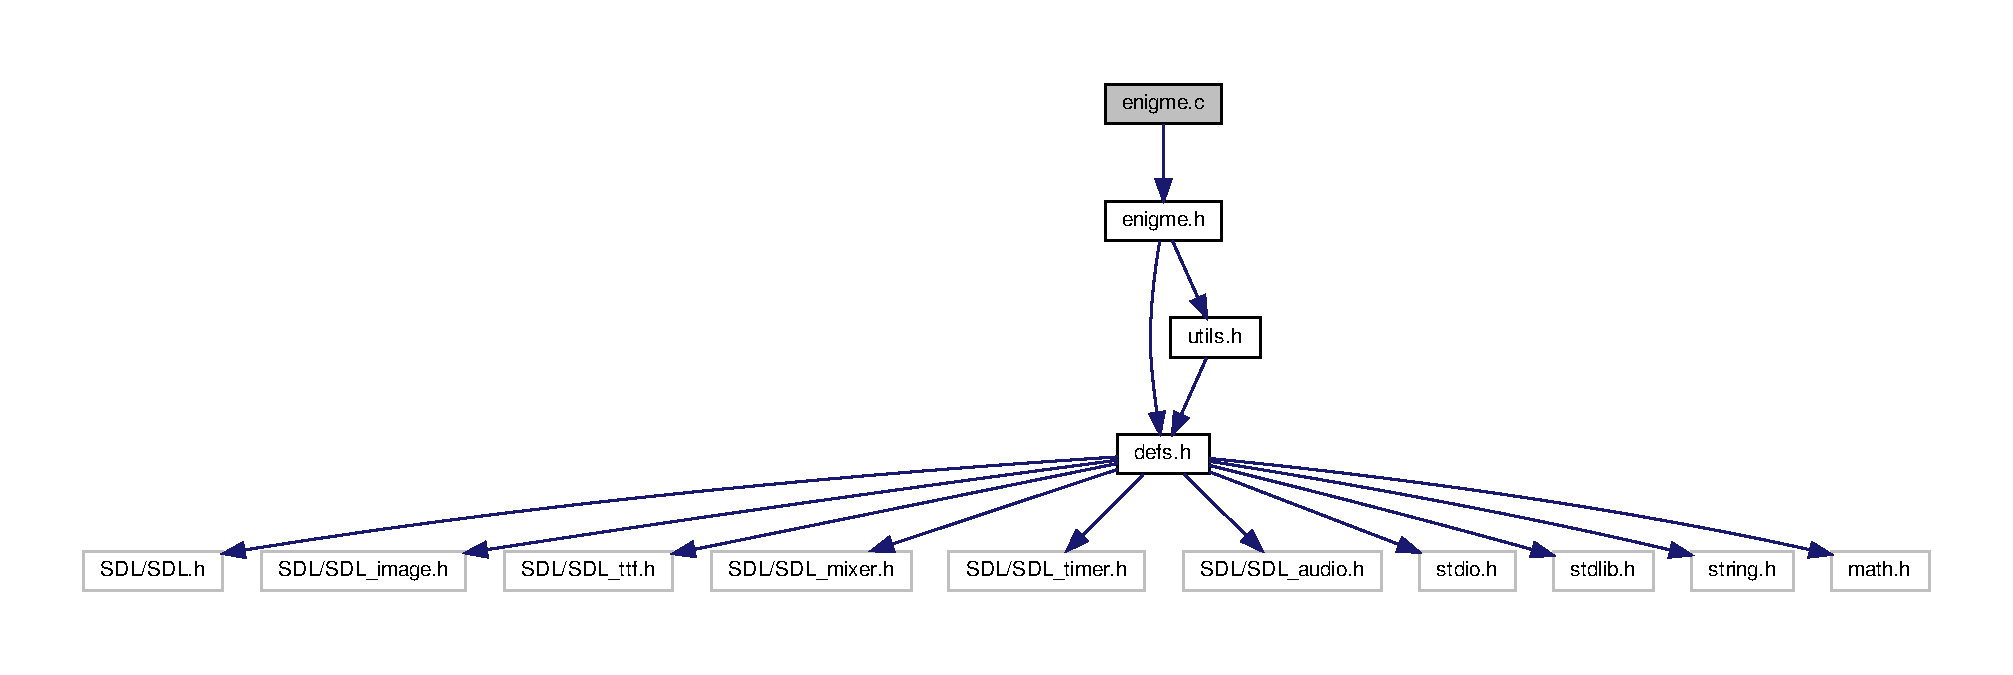
\includegraphics[width=350pt]{enigme_8c__incl}
\end{center}
\end{figure}
\subsection*{Functions}
\begin{DoxyCompactItemize}
\item 
void \hyperlink{enigme_8c_af0a65e8cefe0e02c6f517b180bae0ed0}{afficher\+Enigme} (\hyperlink{enigme_8h_a2d89d638ebefad650660d1b2d48b9b59}{Enigme} \hyperlink{structenigme}{enigme}, S\+D\+L\+\_\+\+Surface $\ast$\hyperlink{defs_8h_a78fa3957d73de49cb81d047857504218}{screen})
\item 
\hyperlink{enigme_8h_a2d89d638ebefad650660d1b2d48b9b59}{Enigme} \hyperlink{enigme_8c_a58bd4f4d8bc3b1e2e40c12cf9bae428d}{generate\+Enigme} (int type)
\item 
\hyperlink{enigme_8h_a2d89d638ebefad650660d1b2d48b9b59}{Enigme} \hyperlink{enigme_8c_abc96cc4f6bd7fb91d730b1f1645d48fa}{load\+Random\+Enigme\+File} ()
\item 
int \hyperlink{enigme_8c_ae11fb46998ec650eef8aed6622f11759}{enigme\+Event\+Handler} (\hyperlink{enigme_8h_a2d89d638ebefad650660d1b2d48b9b59}{Enigme} \hyperlink{structenigme}{enigme}, int type)
\item 
int \hyperlink{enigme_8c_a2d7b4391eaf020561db3a78a2319cae5}{Enigme\+Pipeline} ()
\end{DoxyCompactItemize}


\subsection{Detailed Description}
riddle functions 

\begin{DoxyAuthor}{Author}
Creative Sparks 
\end{DoxyAuthor}
\begin{DoxyVersion}{Version}
2.\+0 
\end{DoxyVersion}
\begin{DoxyDate}{Date}
2020 
\end{DoxyDate}


\subsection{Function Documentation}
\mbox{\Hypertarget{enigme_8c_af0a65e8cefe0e02c6f517b180bae0ed0}\label{enigme_8c_af0a65e8cefe0e02c6f517b180bae0ed0}} 
\index{enigme.\+c@{enigme.\+c}!afficher\+Enigme@{afficher\+Enigme}}
\index{afficher\+Enigme@{afficher\+Enigme}!enigme.\+c@{enigme.\+c}}
\subsubsection{\texorpdfstring{afficher\+Enigme()}{afficherEnigme()}}
{\footnotesize\ttfamily void afficher\+Enigme (\begin{DoxyParamCaption}\item[{\hyperlink{enigme_8h_a2d89d638ebefad650660d1b2d48b9b59}{Enigme}}]{enigme,  }\item[{S\+D\+L\+\_\+\+Surface $\ast$}]{screen }\end{DoxyParamCaption})}

Here is the call graph for this function\+:
\nopagebreak
\begin{figure}[H]
\begin{center}
\leavevmode
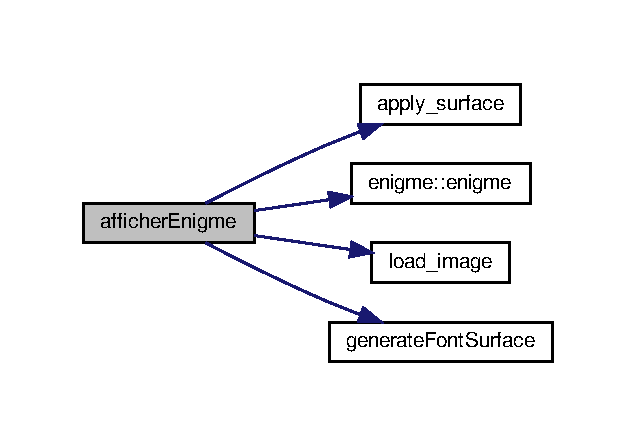
\includegraphics[width=305pt]{enigme_8c_af0a65e8cefe0e02c6f517b180bae0ed0_cgraph}
\end{center}
\end{figure}
Here is the caller graph for this function\+:
\nopagebreak
\begin{figure}[H]
\begin{center}
\leavevmode
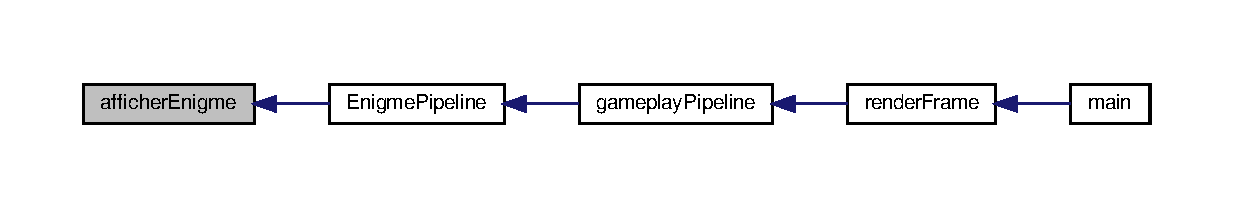
\includegraphics[width=350pt]{enigme_8c_af0a65e8cefe0e02c6f517b180bae0ed0_icgraph}
\end{center}
\end{figure}
\mbox{\Hypertarget{enigme_8c_ae11fb46998ec650eef8aed6622f11759}\label{enigme_8c_ae11fb46998ec650eef8aed6622f11759}} 
\index{enigme.\+c@{enigme.\+c}!enigme\+Event\+Handler@{enigme\+Event\+Handler}}
\index{enigme\+Event\+Handler@{enigme\+Event\+Handler}!enigme.\+c@{enigme.\+c}}
\subsubsection{\texorpdfstring{enigme\+Event\+Handler()}{enigmeEventHandler()}}
{\footnotesize\ttfamily int enigme\+Event\+Handler (\begin{DoxyParamCaption}\item[{\hyperlink{enigme_8h_a2d89d638ebefad650660d1b2d48b9b59}{Enigme}}]{enigme,  }\item[{int}]{type }\end{DoxyParamCaption})}

Here is the call graph for this function\+:
\nopagebreak
\begin{figure}[H]
\begin{center}
\leavevmode
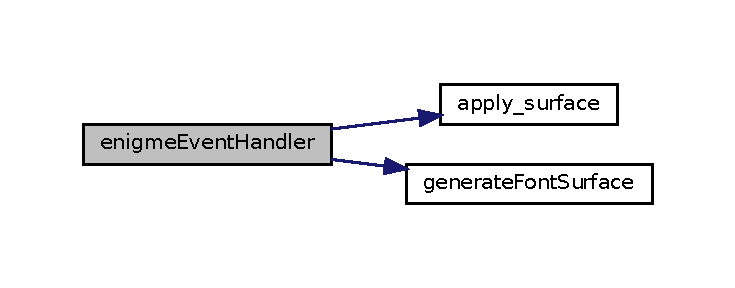
\includegraphics[width=330pt]{enigme_8c_ae11fb46998ec650eef8aed6622f11759_cgraph}
\end{center}
\end{figure}
Here is the caller graph for this function\+:
\nopagebreak
\begin{figure}[H]
\begin{center}
\leavevmode
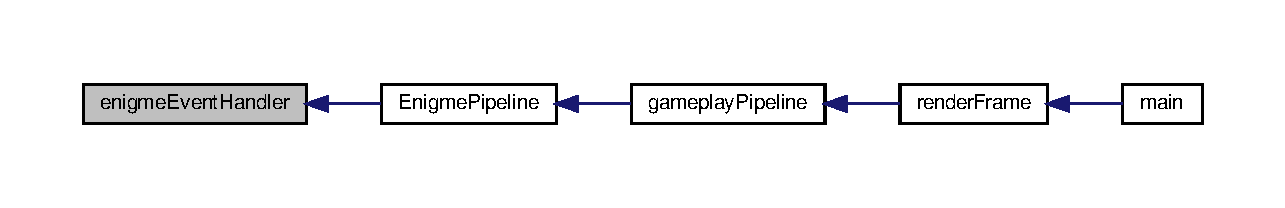
\includegraphics[width=350pt]{enigme_8c_ae11fb46998ec650eef8aed6622f11759_icgraph}
\end{center}
\end{figure}
\mbox{\Hypertarget{enigme_8c_a2d7b4391eaf020561db3a78a2319cae5}\label{enigme_8c_a2d7b4391eaf020561db3a78a2319cae5}} 
\index{enigme.\+c@{enigme.\+c}!Enigme\+Pipeline@{Enigme\+Pipeline}}
\index{Enigme\+Pipeline@{Enigme\+Pipeline}!enigme.\+c@{enigme.\+c}}
\subsubsection{\texorpdfstring{Enigme\+Pipeline()}{EnigmePipeline()}}
{\footnotesize\ttfamily int Enigme\+Pipeline (\begin{DoxyParamCaption}{ }\end{DoxyParamCaption})}

Here is the call graph for this function\+:
\nopagebreak
\begin{figure}[H]
\begin{center}
\leavevmode
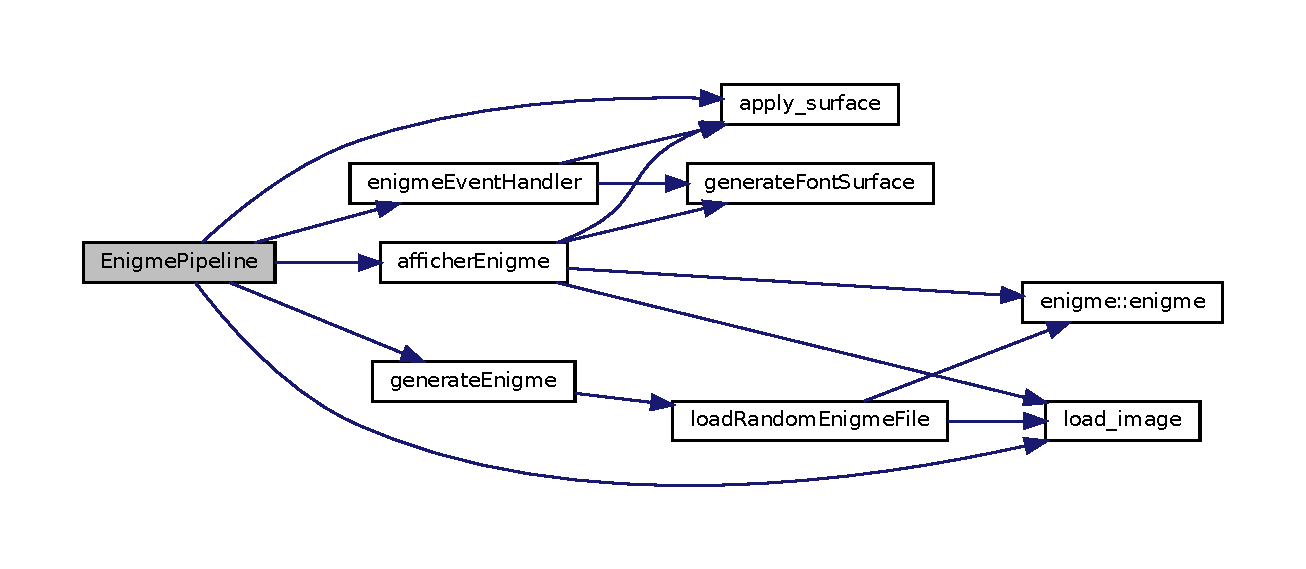
\includegraphics[width=350pt]{enigme_8c_a2d7b4391eaf020561db3a78a2319cae5_cgraph}
\end{center}
\end{figure}
Here is the caller graph for this function\+:
\nopagebreak
\begin{figure}[H]
\begin{center}
\leavevmode
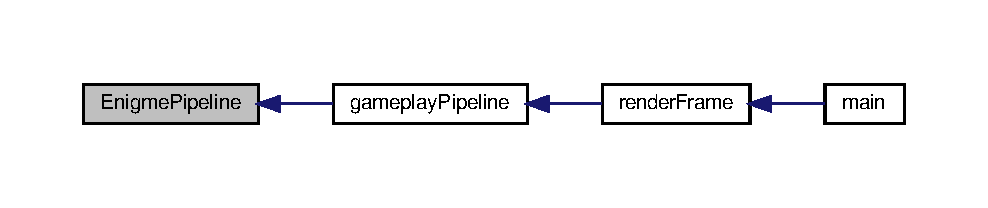
\includegraphics[width=350pt]{enigme_8c_a2d7b4391eaf020561db3a78a2319cae5_icgraph}
\end{center}
\end{figure}
\mbox{\Hypertarget{enigme_8c_a58bd4f4d8bc3b1e2e40c12cf9bae428d}\label{enigme_8c_a58bd4f4d8bc3b1e2e40c12cf9bae428d}} 
\index{enigme.\+c@{enigme.\+c}!generate\+Enigme@{generate\+Enigme}}
\index{generate\+Enigme@{generate\+Enigme}!enigme.\+c@{enigme.\+c}}
\subsubsection{\texorpdfstring{generate\+Enigme()}{generateEnigme()}}
{\footnotesize\ttfamily \hyperlink{enigme_8h_a2d89d638ebefad650660d1b2d48b9b59}{Enigme} generate\+Enigme (\begin{DoxyParamCaption}\item[{int}]{type }\end{DoxyParamCaption})}

Here is the call graph for this function\+:
\nopagebreak
\begin{figure}[H]
\begin{center}
\leavevmode
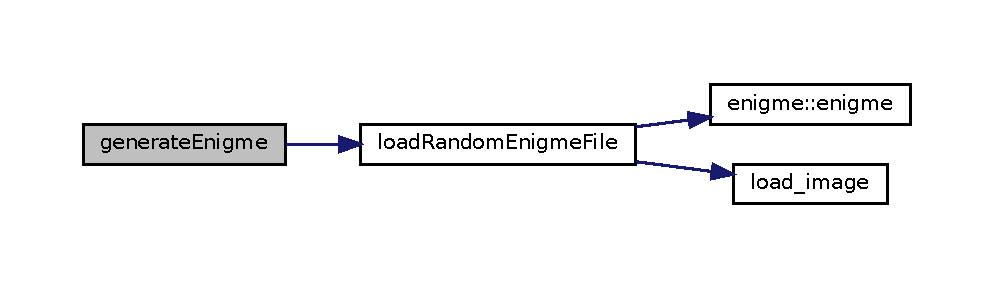
\includegraphics[width=350pt]{enigme_8c_a58bd4f4d8bc3b1e2e40c12cf9bae428d_cgraph}
\end{center}
\end{figure}
Here is the caller graph for this function\+:
\nopagebreak
\begin{figure}[H]
\begin{center}
\leavevmode
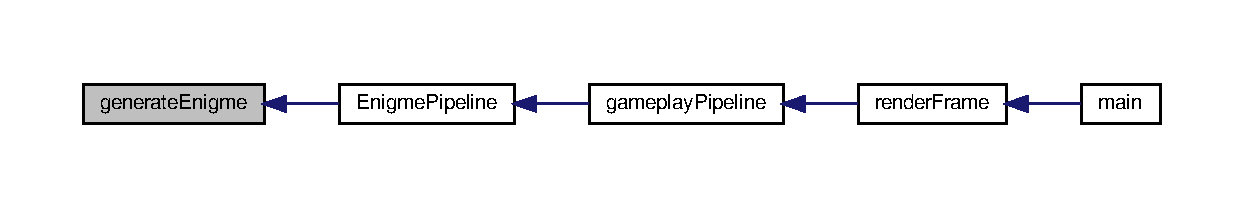
\includegraphics[width=350pt]{enigme_8c_a58bd4f4d8bc3b1e2e40c12cf9bae428d_icgraph}
\end{center}
\end{figure}
\mbox{\Hypertarget{enigme_8c_abc96cc4f6bd7fb91d730b1f1645d48fa}\label{enigme_8c_abc96cc4f6bd7fb91d730b1f1645d48fa}} 
\index{enigme.\+c@{enigme.\+c}!load\+Random\+Enigme\+File@{load\+Random\+Enigme\+File}}
\index{load\+Random\+Enigme\+File@{load\+Random\+Enigme\+File}!enigme.\+c@{enigme.\+c}}
\subsubsection{\texorpdfstring{load\+Random\+Enigme\+File()}{loadRandomEnigmeFile()}}
{\footnotesize\ttfamily \hyperlink{enigme_8h_a2d89d638ebefad650660d1b2d48b9b59}{Enigme} load\+Random\+Enigme\+File (\begin{DoxyParamCaption}{ }\end{DoxyParamCaption})}

Here is the call graph for this function\+:
\nopagebreak
\begin{figure}[H]
\begin{center}
\leavevmode
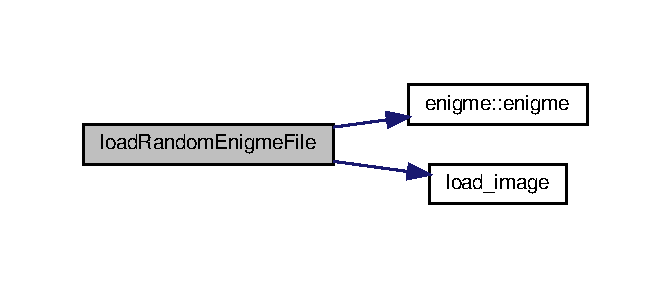
\includegraphics[width=322pt]{enigme_8c_abc96cc4f6bd7fb91d730b1f1645d48fa_cgraph}
\end{center}
\end{figure}
Here is the caller graph for this function\+:
\nopagebreak
\begin{figure}[H]
\begin{center}
\leavevmode
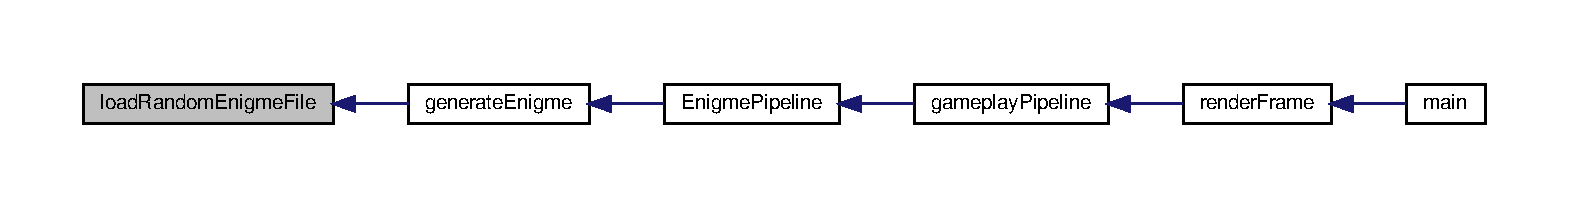
\includegraphics[width=350pt]{enigme_8c_abc96cc4f6bd7fb91d730b1f1645d48fa_icgraph}
\end{center}
\end{figure}

\hypertarget{enigme_8h}{}\doxysection{enigme.\+h File Reference}
\label{enigme_8h}\index{enigme.h@{enigme.h}}


riddle struct and function prototypes  


{\ttfamily \#include \char`\"{}defs.\+h\char`\"{}}\newline
{\ttfamily \#include \char`\"{}utils.\+h\char`\"{}}\newline
Include dependency graph for enigme.\+h\+:\nopagebreak
\begin{figure}[H]
\begin{center}
\leavevmode
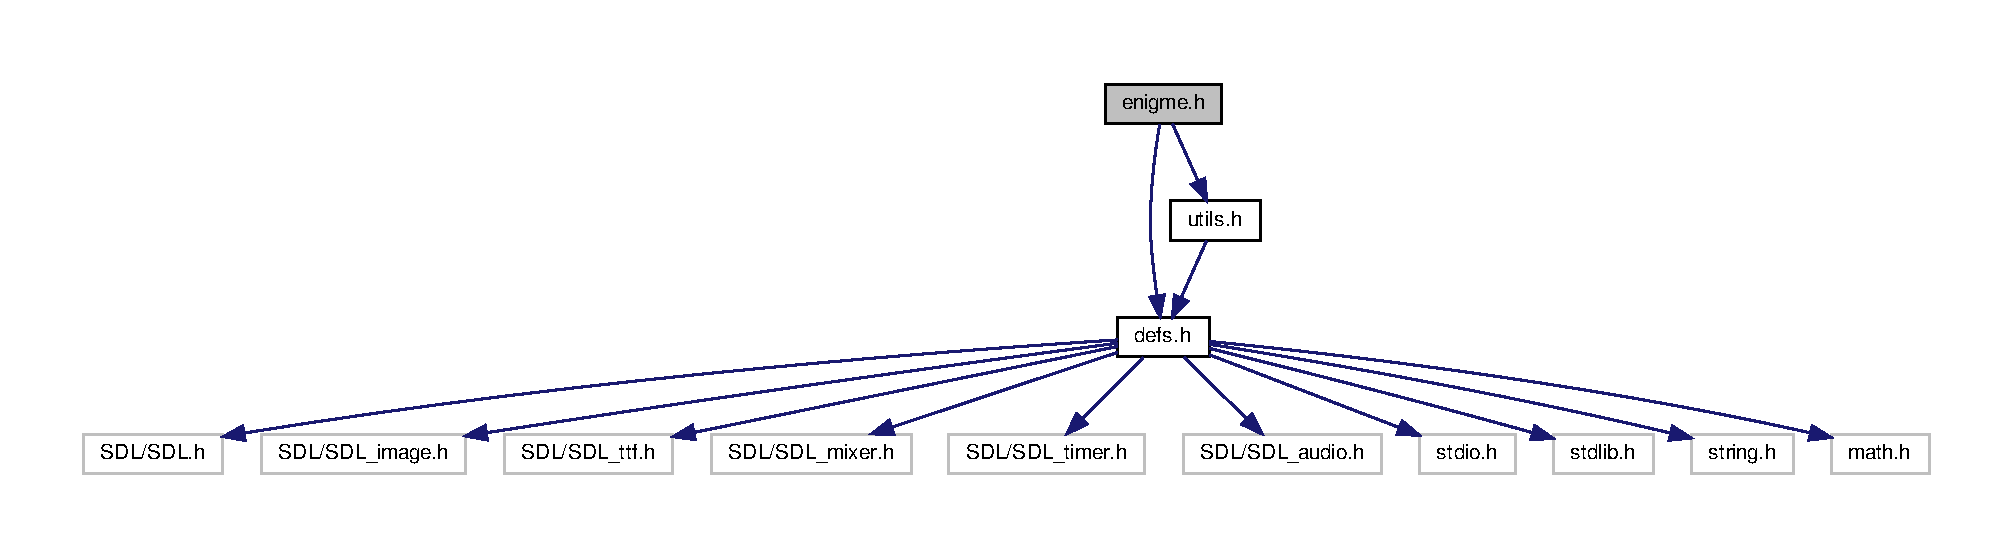
\includegraphics[width=350pt]{enigme_8h__incl}
\end{center}
\end{figure}
This graph shows which files directly or indirectly include this file\+:\nopagebreak
\begin{figure}[H]
\begin{center}
\leavevmode
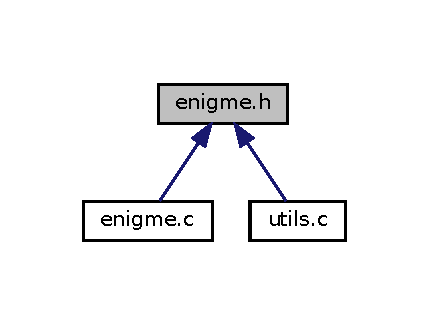
\includegraphics[width=206pt]{enigme_8h__dep__incl}
\end{center}
\end{figure}
\doxysubsection*{Data Structures}
\begin{DoxyCompactItemize}
\item 
struct \mbox{\hyperlink{structenigme}{enigme}}
\begin{DoxyCompactList}\small\item\em struct for riddles \end{DoxyCompactList}\end{DoxyCompactItemize}
\doxysubsection*{Typedefs}
\begin{DoxyCompactItemize}
\item 
typedef struct \mbox{\hyperlink{structenigme}{enigme}} \mbox{\hyperlink{enigme_8h_ae12beb437b3768cf23544f3328d5b47c}{Enigme}}
\end{DoxyCompactItemize}
\doxysubsection*{Functions}
\begin{DoxyCompactItemize}
\item 
void \mbox{\hyperlink{enigme_8h_af0a65e8cefe0e02c6f517b180bae0ed0}{afficher\+Enigme}} (\mbox{\hyperlink{enigme_8h_ae12beb437b3768cf23544f3328d5b47c}{Enigme}} \mbox{\hyperlink{structenigme}{enigme}}, S\+D\+L\+\_\+\+Surface $\ast$\mbox{\hyperlink{defs_8h_a78fa3957d73de49cb81d047857504218}{screen}})
\item 
\mbox{\hyperlink{enigme_8h_ae12beb437b3768cf23544f3328d5b47c}{Enigme}} \mbox{\hyperlink{enigme_8h_a58bd4f4d8bc3b1e2e40c12cf9bae428d}{generate\+Enigme}} (int type)
\item 
\mbox{\hyperlink{enigme_8h_ae12beb437b3768cf23544f3328d5b47c}{Enigme}} \mbox{\hyperlink{enigme_8h_abc96cc4f6bd7fb91d730b1f1645d48fa}{load\+Random\+Enigme\+File}} ()
\item 
int \mbox{\hyperlink{enigme_8h_a7050b8ac91da82758cff189babf9eb7b}{random\+Enigme\+Type}} ()
\item 
void \mbox{\hyperlink{enigme_8h_a58a411faec41430c6c2c34ca17fac37b}{afficher\+Reponse\+Enigme}} (\mbox{\hyperlink{enigme_8h_ae12beb437b3768cf23544f3328d5b47c}{Enigme}} \mbox{\hyperlink{structenigme}{enigme}}, S\+D\+L\+\_\+\+Surface $\ast$\mbox{\hyperlink{defs_8h_a78fa3957d73de49cb81d047857504218}{screen}})
\item 
int \mbox{\hyperlink{enigme_8h_a2d7b4391eaf020561db3a78a2319cae5}{Enigme\+Pipeline}} ()
\end{DoxyCompactItemize}


\doxysubsection{Detailed Description}
riddle struct and function prototypes 

\begin{DoxyAuthor}{Author}
Creative Sparks 
\end{DoxyAuthor}
\begin{DoxyVersion}{Version}
2.\+0 
\end{DoxyVersion}
\begin{DoxyDate}{Date}
2020 
\end{DoxyDate}


\doxysubsection{Typedef Documentation}
\mbox{\Hypertarget{enigme_8h_ae12beb437b3768cf23544f3328d5b47c}\label{enigme_8h_ae12beb437b3768cf23544f3328d5b47c}} 
\index{enigme.h@{enigme.h}!Enigme@{Enigme}}
\index{Enigme@{Enigme}!enigme.h@{enigme.h}}
\doxysubsubsection{\texorpdfstring{Enigme}{Enigme}}
{\footnotesize\ttfamily typedef struct \mbox{\hyperlink{structenigme}{enigme}} \mbox{\hyperlink{enigme_8h_ae12beb437b3768cf23544f3328d5b47c}{Enigme}}}



\doxysubsection{Function Documentation}
\mbox{\Hypertarget{enigme_8h_af0a65e8cefe0e02c6f517b180bae0ed0}\label{enigme_8h_af0a65e8cefe0e02c6f517b180bae0ed0}} 
\index{enigme.h@{enigme.h}!afficherEnigme@{afficherEnigme}}
\index{afficherEnigme@{afficherEnigme}!enigme.h@{enigme.h}}
\doxysubsubsection{\texorpdfstring{afficherEnigme()}{afficherEnigme()}}
{\footnotesize\ttfamily void afficher\+Enigme (\begin{DoxyParamCaption}\item[{\mbox{\hyperlink{enigme_8h_ae12beb437b3768cf23544f3328d5b47c}{Enigme}}}]{enigme,  }\item[{S\+D\+L\+\_\+\+Surface $\ast$}]{screen }\end{DoxyParamCaption})}

Here is the call graph for this function\+:\nopagebreak
\begin{figure}[H]
\begin{center}
\leavevmode
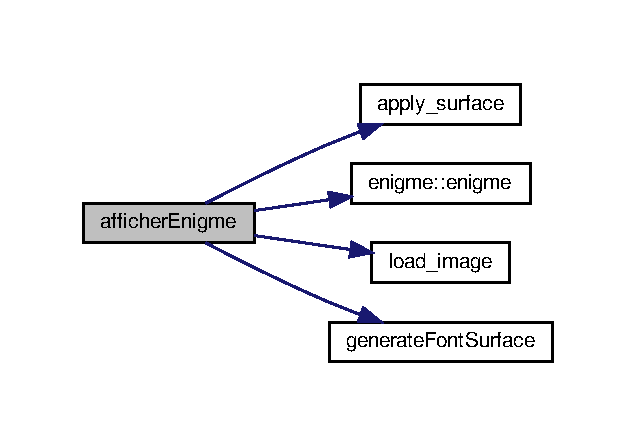
\includegraphics[width=324pt]{enigme_8h_af0a65e8cefe0e02c6f517b180bae0ed0_cgraph}
\end{center}
\end{figure}
Here is the caller graph for this function\+:\nopagebreak
\begin{figure}[H]
\begin{center}
\leavevmode
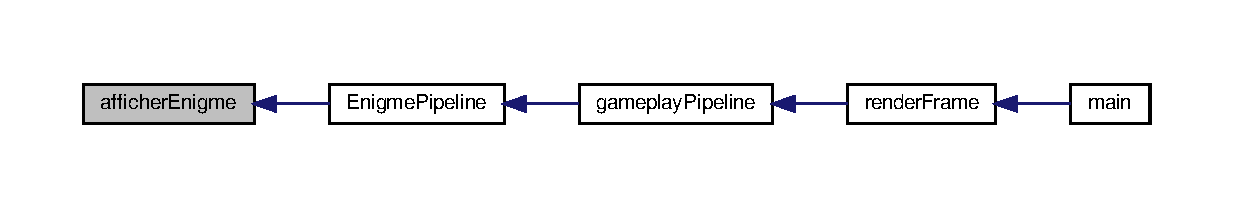
\includegraphics[width=350pt]{enigme_8h_af0a65e8cefe0e02c6f517b180bae0ed0_icgraph}
\end{center}
\end{figure}
\mbox{\Hypertarget{enigme_8h_a58a411faec41430c6c2c34ca17fac37b}\label{enigme_8h_a58a411faec41430c6c2c34ca17fac37b}} 
\index{enigme.h@{enigme.h}!afficherReponseEnigme@{afficherReponseEnigme}}
\index{afficherReponseEnigme@{afficherReponseEnigme}!enigme.h@{enigme.h}}
\doxysubsubsection{\texorpdfstring{afficherReponseEnigme()}{afficherReponseEnigme()}}
{\footnotesize\ttfamily void afficher\+Reponse\+Enigme (\begin{DoxyParamCaption}\item[{\mbox{\hyperlink{enigme_8h_ae12beb437b3768cf23544f3328d5b47c}{Enigme}}}]{enigme,  }\item[{S\+D\+L\+\_\+\+Surface $\ast$}]{screen }\end{DoxyParamCaption})}

\mbox{\Hypertarget{enigme_8h_a2d7b4391eaf020561db3a78a2319cae5}\label{enigme_8h_a2d7b4391eaf020561db3a78a2319cae5}} 
\index{enigme.h@{enigme.h}!EnigmePipeline@{EnigmePipeline}}
\index{EnigmePipeline@{EnigmePipeline}!enigme.h@{enigme.h}}
\doxysubsubsection{\texorpdfstring{EnigmePipeline()}{EnigmePipeline()}}
{\footnotesize\ttfamily int Enigme\+Pipeline (\begin{DoxyParamCaption}{ }\end{DoxyParamCaption})}

Here is the call graph for this function\+:\nopagebreak
\begin{figure}[H]
\begin{center}
\leavevmode
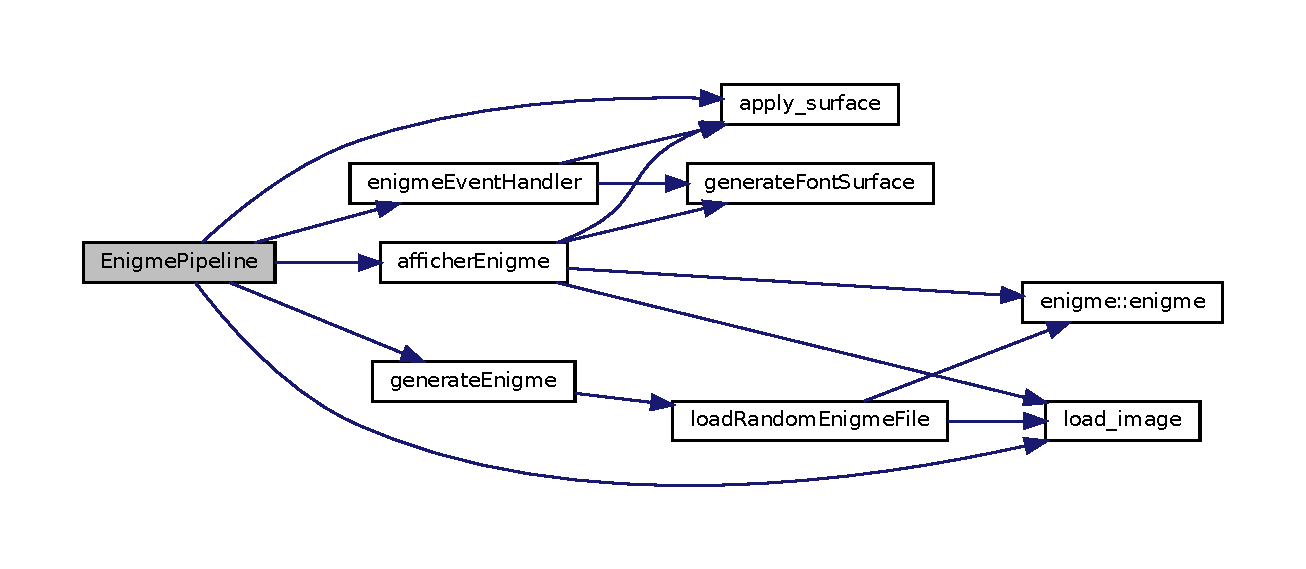
\includegraphics[width=350pt]{enigme_8h_a2d7b4391eaf020561db3a78a2319cae5_cgraph}
\end{center}
\end{figure}
Here is the caller graph for this function\+:\nopagebreak
\begin{figure}[H]
\begin{center}
\leavevmode
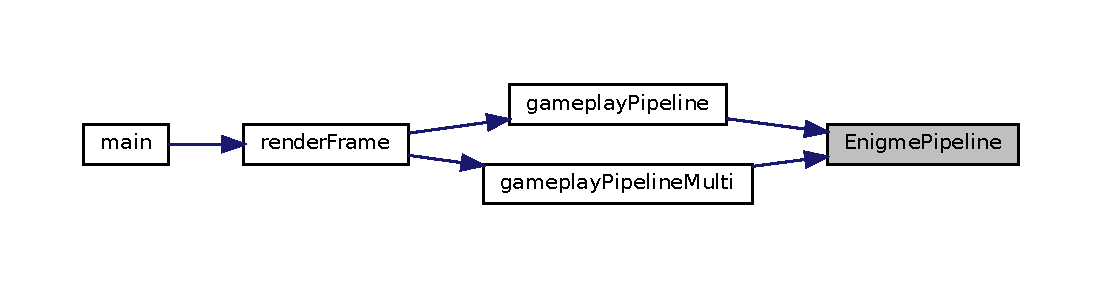
\includegraphics[width=350pt]{enigme_8h_a2d7b4391eaf020561db3a78a2319cae5_icgraph}
\end{center}
\end{figure}
\mbox{\Hypertarget{enigme_8h_a58bd4f4d8bc3b1e2e40c12cf9bae428d}\label{enigme_8h_a58bd4f4d8bc3b1e2e40c12cf9bae428d}} 
\index{enigme.h@{enigme.h}!generateEnigme@{generateEnigme}}
\index{generateEnigme@{generateEnigme}!enigme.h@{enigme.h}}
\doxysubsubsection{\texorpdfstring{generateEnigme()}{generateEnigme()}}
{\footnotesize\ttfamily \mbox{\hyperlink{enigme_8h_ae12beb437b3768cf23544f3328d5b47c}{Enigme}} generate\+Enigme (\begin{DoxyParamCaption}\item[{int}]{type }\end{DoxyParamCaption})}

Here is the call graph for this function\+:\nopagebreak
\begin{figure}[H]
\begin{center}
\leavevmode
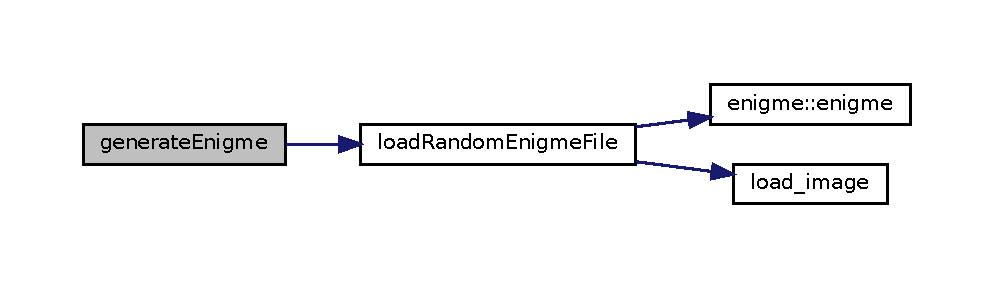
\includegraphics[width=350pt]{enigme_8h_a58bd4f4d8bc3b1e2e40c12cf9bae428d_cgraph}
\end{center}
\end{figure}
Here is the caller graph for this function\+:\nopagebreak
\begin{figure}[H]
\begin{center}
\leavevmode
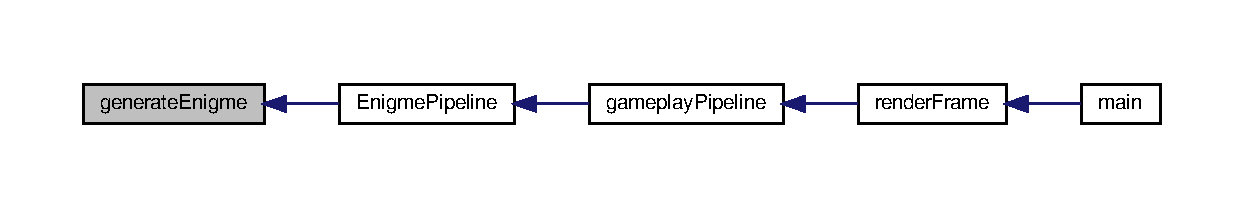
\includegraphics[width=350pt]{enigme_8h_a58bd4f4d8bc3b1e2e40c12cf9bae428d_icgraph}
\end{center}
\end{figure}
\mbox{\Hypertarget{enigme_8h_abc96cc4f6bd7fb91d730b1f1645d48fa}\label{enigme_8h_abc96cc4f6bd7fb91d730b1f1645d48fa}} 
\index{enigme.h@{enigme.h}!loadRandomEnigmeFile@{loadRandomEnigmeFile}}
\index{loadRandomEnigmeFile@{loadRandomEnigmeFile}!enigme.h@{enigme.h}}
\doxysubsubsection{\texorpdfstring{loadRandomEnigmeFile()}{loadRandomEnigmeFile()}}
{\footnotesize\ttfamily \mbox{\hyperlink{enigme_8h_ae12beb437b3768cf23544f3328d5b47c}{Enigme}} load\+Random\+Enigme\+File (\begin{DoxyParamCaption}{ }\end{DoxyParamCaption})}

Here is the call graph for this function\+:\nopagebreak
\begin{figure}[H]
\begin{center}
\leavevmode
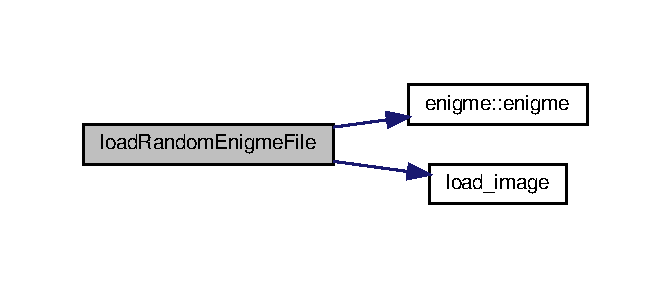
\includegraphics[width=344pt]{enigme_8h_abc96cc4f6bd7fb91d730b1f1645d48fa_cgraph}
\end{center}
\end{figure}
Here is the caller graph for this function\+:\nopagebreak
\begin{figure}[H]
\begin{center}
\leavevmode
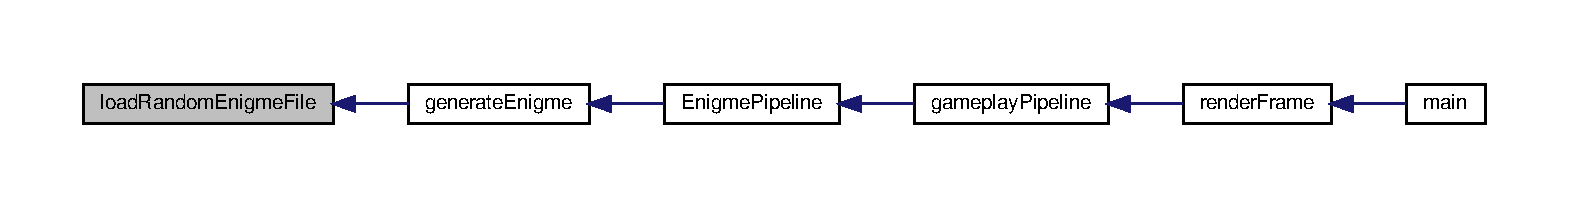
\includegraphics[width=350pt]{enigme_8h_abc96cc4f6bd7fb91d730b1f1645d48fa_icgraph}
\end{center}
\end{figure}
\mbox{\Hypertarget{enigme_8h_a7050b8ac91da82758cff189babf9eb7b}\label{enigme_8h_a7050b8ac91da82758cff189babf9eb7b}} 
\index{enigme.h@{enigme.h}!randomEnigmeType@{randomEnigmeType}}
\index{randomEnigmeType@{randomEnigmeType}!enigme.h@{enigme.h}}
\doxysubsubsection{\texorpdfstring{randomEnigmeType()}{randomEnigmeType()}}
{\footnotesize\ttfamily int random\+Enigme\+Type (\begin{DoxyParamCaption}{ }\end{DoxyParamCaption})}


\hypertarget{ennemies_8c}{}\doxysection{ennemies.\+c File Reference}
\label{ennemies_8c}\index{ennemies.c@{ennemies.c}}


game ennemies functions  


{\ttfamily \#include \char`\"{}ennemies.\+h\char`\"{}}\newline
Include dependency graph for ennemies.\+c\+:
\nopagebreak
\begin{figure}[H]
\begin{center}
\leavevmode
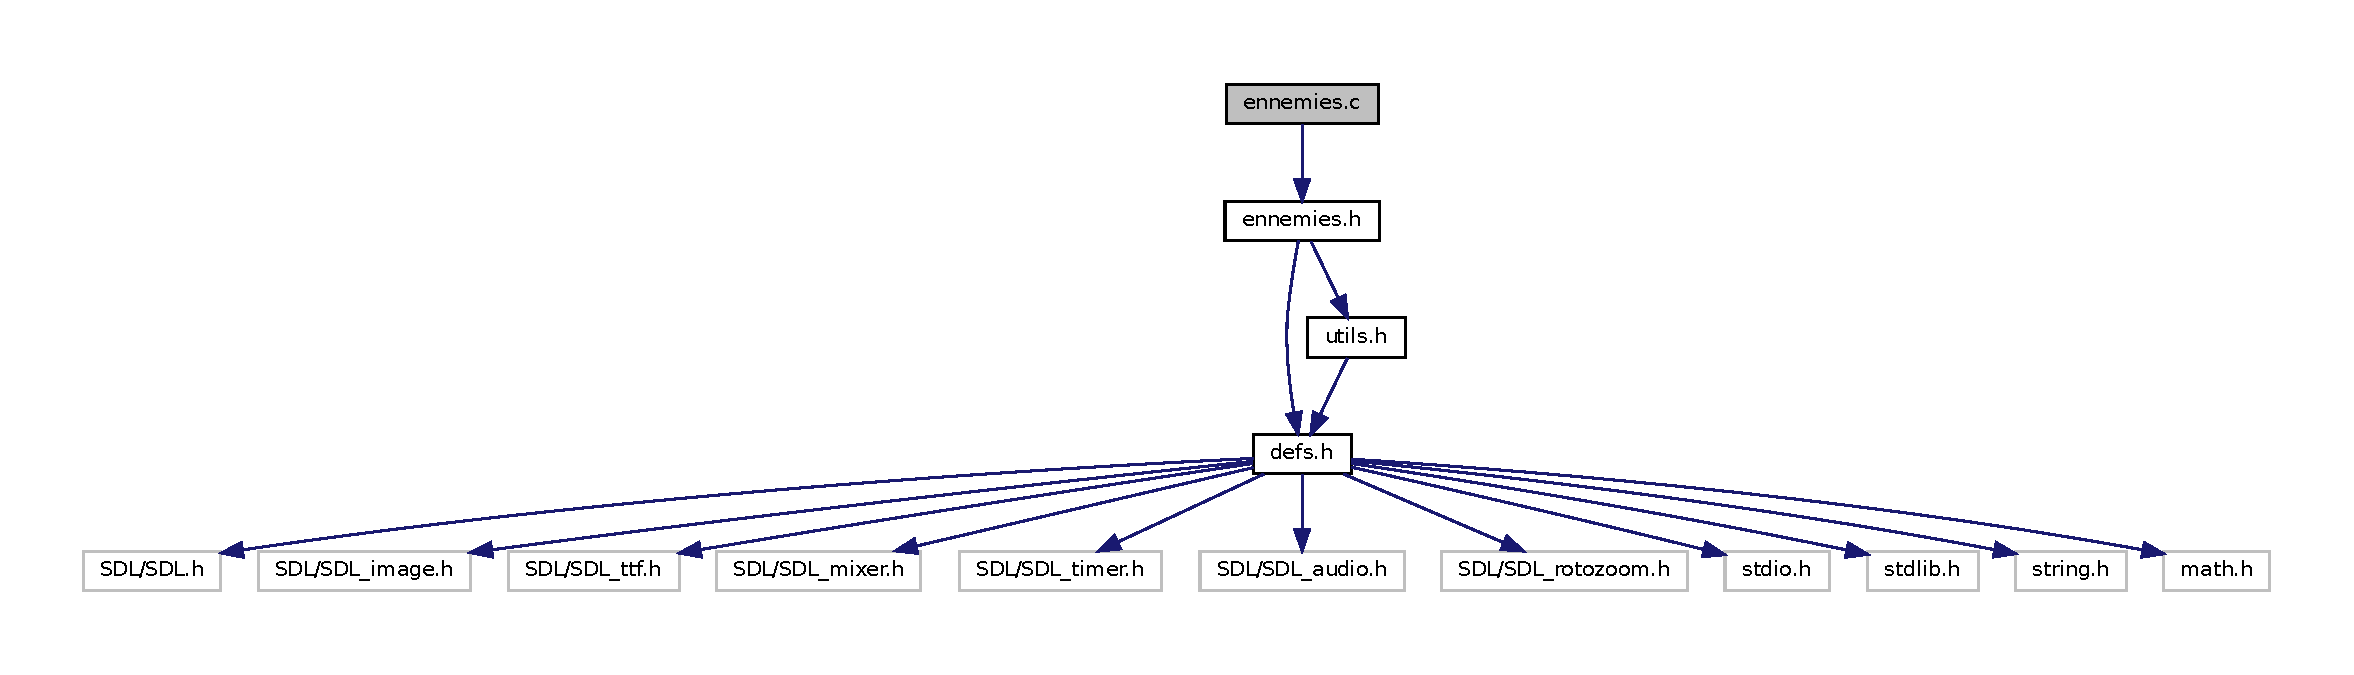
\includegraphics[width=350pt]{ennemies_8c__incl}
\end{center}
\end{figure}
\doxysubsection*{Functions}
\begin{DoxyCompactItemize}
\item 
void \mbox{\hyperlink{ennemies_8c_a6d3dff72d16d48b241a64beec64bec02}{init\+Ennemi}} ()
\item 
void \mbox{\hyperlink{ennemies_8c_aeb2c0786744d55f91bc0dec00529aa7e}{affiche\+Ennemi}} (\mbox{\hyperlink{ennemies_8h_abc1d765bf177d92e054b9d9300b3ccef}{Ennemi}} \mbox{\hyperlink{structennemi}{ennemi}}, S\+D\+L\+\_\+\+Surface $\ast$\mbox{\hyperlink{defs_8h_a68389876c2746622931d187c587f9c4d}{background}})
\item 
\mbox{\hyperlink{ennemies_8h_abc1d765bf177d92e054b9d9300b3ccef}{Ennemi}} \mbox{\hyperlink{ennemies_8c_aa135ada285717b081855f13fb28bc66d}{load\+Sprite\+Ennemi}} (\mbox{\hyperlink{ennemies_8h_abc1d765bf177d92e054b9d9300b3ccef}{Ennemi}} \mbox{\hyperlink{structennemi}{ennemi}}, int direction)
\item 
void \mbox{\hyperlink{ennemies_8c_a3e7af8f799598c7440a820f5ba987187}{remplir\+Tableau\+Ennemi}} ()
\item 
\mbox{\hyperlink{ennemies_8h_abc1d765bf177d92e054b9d9300b3ccef}{Ennemi}} \mbox{\hyperlink{ennemies_8c_a67e4532e5a85ff89b0c393eb8cc7d614}{kill\+Ennemy}} (\mbox{\hyperlink{ennemies_8h_abc1d765bf177d92e054b9d9300b3ccef}{Ennemi}} \mbox{\hyperlink{structennemi}{ennemi}})
\end{DoxyCompactItemize}
\doxysubsection*{Variables}
\begin{DoxyCompactItemize}
\item 
\mbox{\hyperlink{ennemies_8h_abc1d765bf177d92e054b9d9300b3ccef}{Ennemi}} \mbox{\hyperlink{ennemies_8c_a3265575f87f7ec5947038321649ab4f2}{ennemi1}}
\item 
\mbox{\hyperlink{ennemies_8h_abc1d765bf177d92e054b9d9300b3ccef}{Ennemi}} \mbox{\hyperlink{ennemies_8c_a8b157a88dfbb24c7429fe2402dd445cd}{ennemi2}}
\item 
\mbox{\hyperlink{ennemies_8h_abc1d765bf177d92e054b9d9300b3ccef}{Ennemi}} \mbox{\hyperlink{ennemies_8c_a6450eb83dade425dcce0f0140d13c006}{ennemi3}}
\item 
\mbox{\hyperlink{ennemies_8h_abc1d765bf177d92e054b9d9300b3ccef}{Ennemi}} \mbox{\hyperlink{ennemies_8c_a1b5308e605c6653994430968c3dffed4}{ennemi4}}
\item 
\mbox{\hyperlink{ennemies_8h_abc1d765bf177d92e054b9d9300b3ccef}{Ennemi}} \mbox{\hyperlink{ennemies_8c_a141ba58c74a730d20dd02bcd067daf0a}{ennemis}} \mbox{[}2\mbox{]}
\end{DoxyCompactItemize}


\doxysubsection{Detailed Description}
game ennemies functions 

\begin{DoxyAuthor}{Author}
Creative Sparks 
\end{DoxyAuthor}
\begin{DoxyVersion}{Version}
2.\+0 
\end{DoxyVersion}
\begin{DoxyDate}{Date}
2020 
\end{DoxyDate}


\doxysubsection{Function Documentation}
\mbox{\Hypertarget{ennemies_8c_aeb2c0786744d55f91bc0dec00529aa7e}\label{ennemies_8c_aeb2c0786744d55f91bc0dec00529aa7e}} 
\index{ennemies.c@{ennemies.c}!afficheEnnemi@{afficheEnnemi}}
\index{afficheEnnemi@{afficheEnnemi}!ennemies.c@{ennemies.c}}
\doxysubsubsection{\texorpdfstring{afficheEnnemi()}{afficheEnnemi()}}
{\footnotesize\ttfamily void affiche\+Ennemi (\begin{DoxyParamCaption}\item[{\mbox{\hyperlink{ennemies_8h_abc1d765bf177d92e054b9d9300b3ccef}{Ennemi}}}]{ennemi,  }\item[{S\+D\+L\+\_\+\+Surface $\ast$}]{background }\end{DoxyParamCaption})}

Here is the call graph for this function\+:
\nopagebreak
\begin{figure}[H]
\begin{center}
\leavevmode
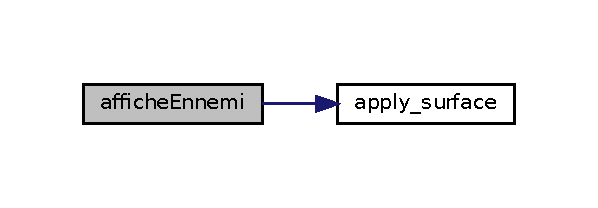
\includegraphics[width=287pt]{ennemies_8c_aeb2c0786744d55f91bc0dec00529aa7e_cgraph}
\end{center}
\end{figure}
Here is the caller graph for this function\+:
\nopagebreak
\begin{figure}[H]
\begin{center}
\leavevmode
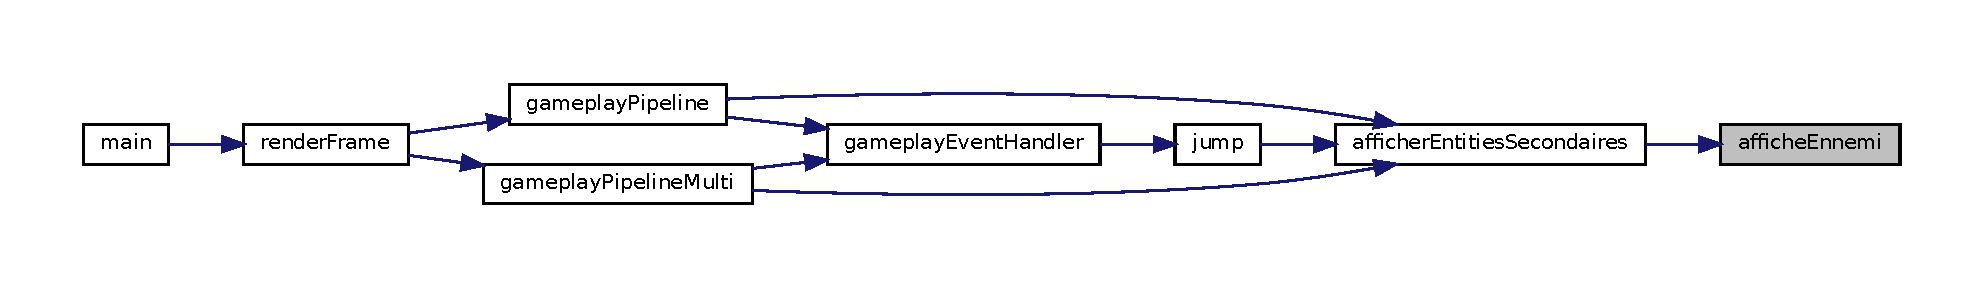
\includegraphics[width=350pt]{ennemies_8c_aeb2c0786744d55f91bc0dec00529aa7e_icgraph}
\end{center}
\end{figure}
\mbox{\Hypertarget{ennemies_8c_a6d3dff72d16d48b241a64beec64bec02}\label{ennemies_8c_a6d3dff72d16d48b241a64beec64bec02}} 
\index{ennemies.c@{ennemies.c}!initEnnemi@{initEnnemi}}
\index{initEnnemi@{initEnnemi}!ennemies.c@{ennemies.c}}
\doxysubsubsection{\texorpdfstring{initEnnemi()}{initEnnemi()}}
{\footnotesize\ttfamily void init\+Ennemi (\begin{DoxyParamCaption}{ }\end{DoxyParamCaption})}

Here is the caller graph for this function\+:
\nopagebreak
\begin{figure}[H]
\begin{center}
\leavevmode
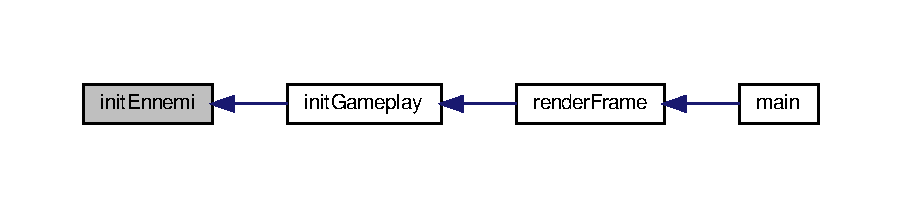
\includegraphics[width=350pt]{ennemies_8c_a6d3dff72d16d48b241a64beec64bec02_icgraph}
\end{center}
\end{figure}
\mbox{\Hypertarget{ennemies_8c_a67e4532e5a85ff89b0c393eb8cc7d614}\label{ennemies_8c_a67e4532e5a85ff89b0c393eb8cc7d614}} 
\index{ennemies.c@{ennemies.c}!killEnnemy@{killEnnemy}}
\index{killEnnemy@{killEnnemy}!ennemies.c@{ennemies.c}}
\doxysubsubsection{\texorpdfstring{killEnnemy()}{killEnnemy()}}
{\footnotesize\ttfamily \mbox{\hyperlink{ennemies_8h_abc1d765bf177d92e054b9d9300b3ccef}{Ennemi}} kill\+Ennemy (\begin{DoxyParamCaption}\item[{\mbox{\hyperlink{ennemies_8h_abc1d765bf177d92e054b9d9300b3ccef}{Ennemi}}}]{ennemi }\end{DoxyParamCaption})}

Here is the caller graph for this function\+:
\nopagebreak
\begin{figure}[H]
\begin{center}
\leavevmode
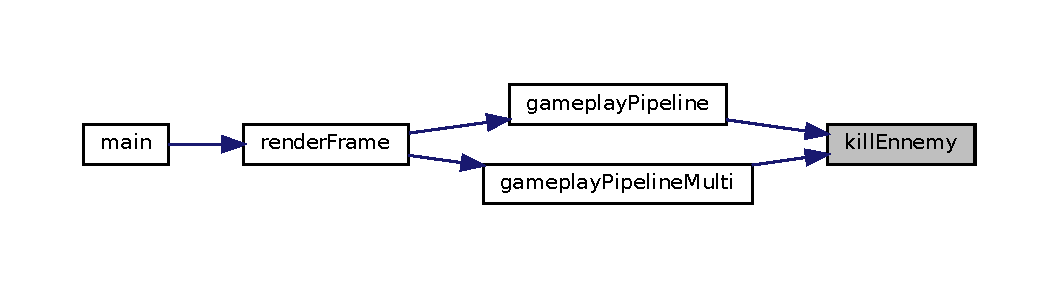
\includegraphics[width=350pt]{ennemies_8c_a67e4532e5a85ff89b0c393eb8cc7d614_icgraph}
\end{center}
\end{figure}
\mbox{\Hypertarget{ennemies_8c_aa135ada285717b081855f13fb28bc66d}\label{ennemies_8c_aa135ada285717b081855f13fb28bc66d}} 
\index{ennemies.c@{ennemies.c}!loadSpriteEnnemi@{loadSpriteEnnemi}}
\index{loadSpriteEnnemi@{loadSpriteEnnemi}!ennemies.c@{ennemies.c}}
\doxysubsubsection{\texorpdfstring{loadSpriteEnnemi()}{loadSpriteEnnemi()}}
{\footnotesize\ttfamily \mbox{\hyperlink{ennemies_8h_abc1d765bf177d92e054b9d9300b3ccef}{Ennemi}} load\+Sprite\+Ennemi (\begin{DoxyParamCaption}\item[{\mbox{\hyperlink{ennemies_8h_abc1d765bf177d92e054b9d9300b3ccef}{Ennemi}}}]{ennemi,  }\item[{int}]{direction }\end{DoxyParamCaption})}

Here is the call graph for this function\+:
\nopagebreak
\begin{figure}[H]
\begin{center}
\leavevmode
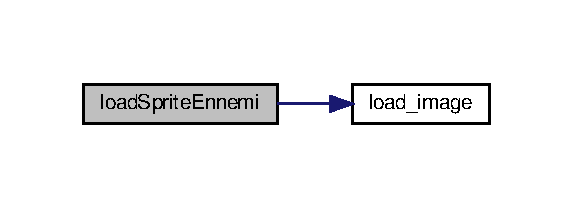
\includegraphics[width=293pt]{ennemies_8c_aa135ada285717b081855f13fb28bc66d_cgraph}
\end{center}
\end{figure}
Here is the caller graph for this function\+:
\nopagebreak
\begin{figure}[H]
\begin{center}
\leavevmode
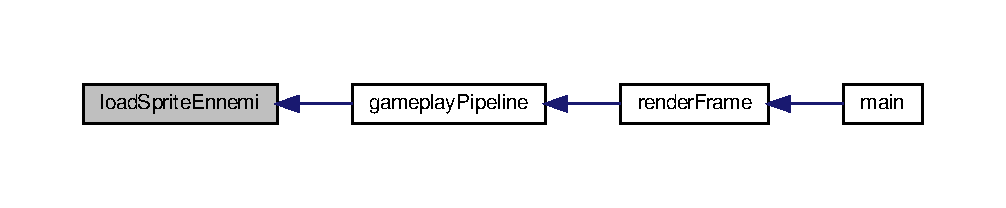
\includegraphics[width=350pt]{ennemies_8c_aa135ada285717b081855f13fb28bc66d_icgraph}
\end{center}
\end{figure}
\mbox{\Hypertarget{ennemies_8c_a3e7af8f799598c7440a820f5ba987187}\label{ennemies_8c_a3e7af8f799598c7440a820f5ba987187}} 
\index{ennemies.c@{ennemies.c}!remplirTableauEnnemi@{remplirTableauEnnemi}}
\index{remplirTableauEnnemi@{remplirTableauEnnemi}!ennemies.c@{ennemies.c}}
\doxysubsubsection{\texorpdfstring{remplirTableauEnnemi()}{remplirTableauEnnemi()}}
{\footnotesize\ttfamily void remplir\+Tableau\+Ennemi (\begin{DoxyParamCaption}{ }\end{DoxyParamCaption})}



\doxysubsection{Variable Documentation}
\mbox{\Hypertarget{ennemies_8c_a3265575f87f7ec5947038321649ab4f2}\label{ennemies_8c_a3265575f87f7ec5947038321649ab4f2}} 
\index{ennemies.c@{ennemies.c}!ennemi1@{ennemi1}}
\index{ennemi1@{ennemi1}!ennemies.c@{ennemies.c}}
\doxysubsubsection{\texorpdfstring{ennemi1}{ennemi1}}
{\footnotesize\ttfamily \mbox{\hyperlink{ennemies_8h_abc1d765bf177d92e054b9d9300b3ccef}{Ennemi}} ennemi1}

\mbox{\Hypertarget{ennemies_8c_a8b157a88dfbb24c7429fe2402dd445cd}\label{ennemies_8c_a8b157a88dfbb24c7429fe2402dd445cd}} 
\index{ennemies.c@{ennemies.c}!ennemi2@{ennemi2}}
\index{ennemi2@{ennemi2}!ennemies.c@{ennemies.c}}
\doxysubsubsection{\texorpdfstring{ennemi2}{ennemi2}}
{\footnotesize\ttfamily \mbox{\hyperlink{ennemies_8h_abc1d765bf177d92e054b9d9300b3ccef}{Ennemi}} ennemi2}

\mbox{\Hypertarget{ennemies_8c_a6450eb83dade425dcce0f0140d13c006}\label{ennemies_8c_a6450eb83dade425dcce0f0140d13c006}} 
\index{ennemies.c@{ennemies.c}!ennemi3@{ennemi3}}
\index{ennemi3@{ennemi3}!ennemies.c@{ennemies.c}}
\doxysubsubsection{\texorpdfstring{ennemi3}{ennemi3}}
{\footnotesize\ttfamily \mbox{\hyperlink{ennemies_8h_abc1d765bf177d92e054b9d9300b3ccef}{Ennemi}} ennemi3}

\mbox{\Hypertarget{ennemies_8c_a1b5308e605c6653994430968c3dffed4}\label{ennemies_8c_a1b5308e605c6653994430968c3dffed4}} 
\index{ennemies.c@{ennemies.c}!ennemi4@{ennemi4}}
\index{ennemi4@{ennemi4}!ennemies.c@{ennemies.c}}
\doxysubsubsection{\texorpdfstring{ennemi4}{ennemi4}}
{\footnotesize\ttfamily \mbox{\hyperlink{ennemies_8h_abc1d765bf177d92e054b9d9300b3ccef}{Ennemi}} ennemi4}

\mbox{\Hypertarget{ennemies_8c_a141ba58c74a730d20dd02bcd067daf0a}\label{ennemies_8c_a141ba58c74a730d20dd02bcd067daf0a}} 
\index{ennemies.c@{ennemies.c}!ennemis@{ennemis}}
\index{ennemis@{ennemis}!ennemies.c@{ennemies.c}}
\doxysubsubsection{\texorpdfstring{ennemis}{ennemis}}
{\footnotesize\ttfamily \mbox{\hyperlink{ennemies_8h_abc1d765bf177d92e054b9d9300b3ccef}{Ennemi}} ennemis\mbox{[}2\mbox{]}}


\hypertarget{ennemies_8h}{}\section{ennemies.\+h File Reference}
\label{ennemies_8h}\index{ennemies.\+h@{ennemies.\+h}}


ennemies struct and function prototypes  


{\ttfamily \#include \char`\"{}defs.\+h\char`\"{}}\newline
{\ttfamily \#include \char`\"{}utils.\+h\char`\"{}}\newline
Include dependency graph for ennemies.\+h\+:\nopagebreak
\begin{figure}[H]
\begin{center}
\leavevmode
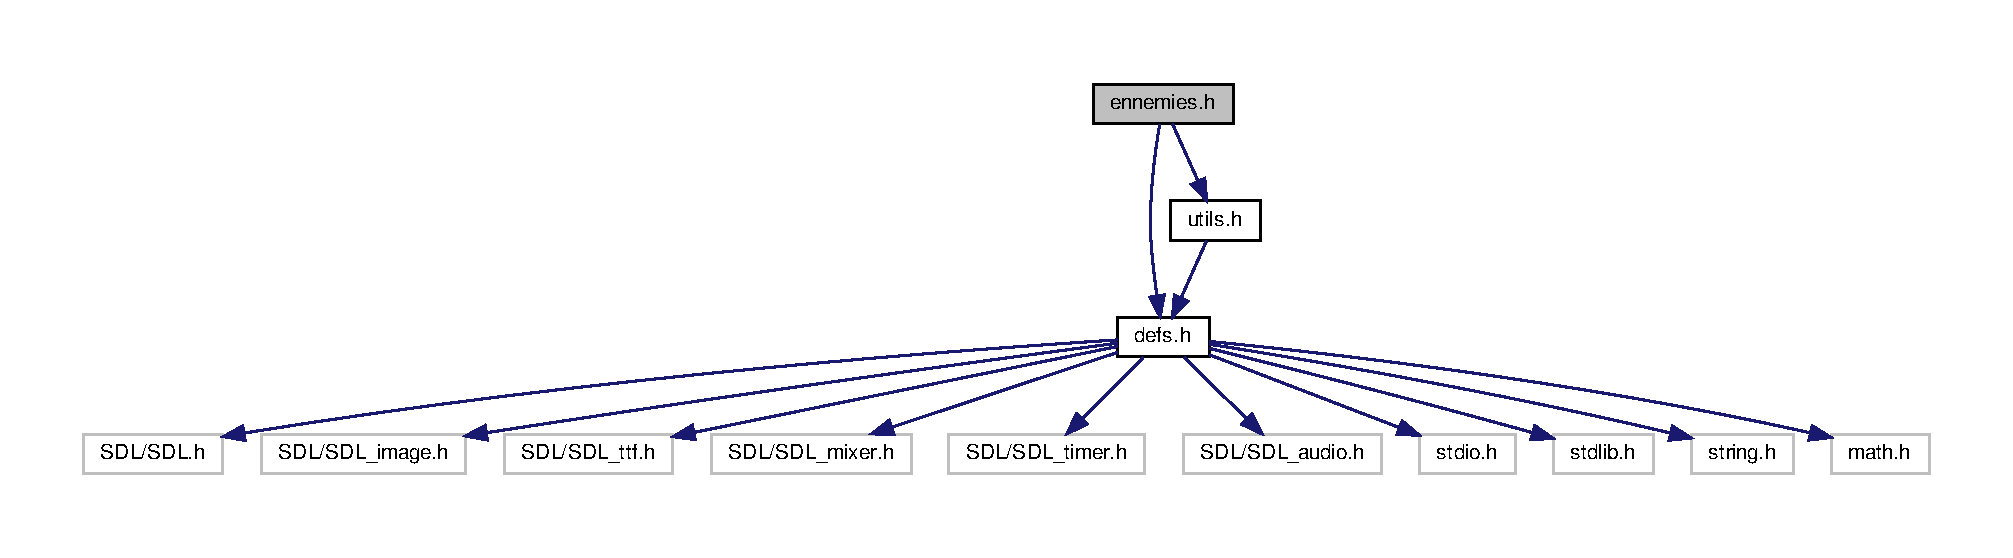
\includegraphics[width=350pt]{ennemies_8h__incl}
\end{center}
\end{figure}
This graph shows which files directly or indirectly include this file\+:
\nopagebreak
\begin{figure}[H]
\begin{center}
\leavevmode
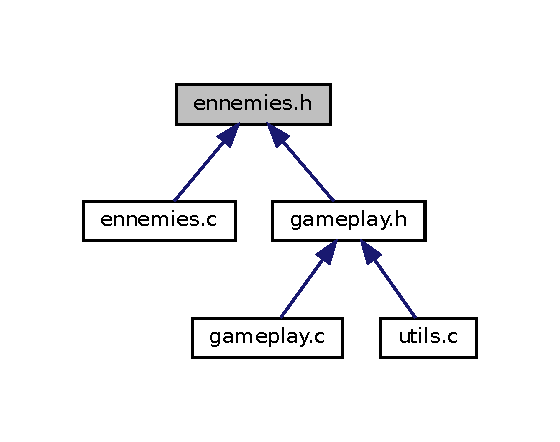
\includegraphics[width=256pt]{ennemies_8h__dep__incl}
\end{center}
\end{figure}
\subsection*{Data Structures}
\begin{DoxyCompactItemize}
\item 
struct \hyperlink{structennemi}{ennemi}
\end{DoxyCompactItemize}
\subsection*{Typedefs}
\begin{DoxyCompactItemize}
\item 
typedef struct \hyperlink{structennemi}{ennemi} \hyperlink{ennemies_8h_af688767ec0f4fdaa755e7f542c2d272d}{Ennemi}
\end{DoxyCompactItemize}
\subsection*{Functions}
\begin{DoxyCompactItemize}
\item 
void \hyperlink{ennemies_8h_aeb2c0786744d55f91bc0dec00529aa7e}{affiche\+Ennemi} (\hyperlink{ennemies_8h_af688767ec0f4fdaa755e7f542c2d272d}{Ennemi} \hyperlink{structennemi}{ennemi}, S\+D\+L\+\_\+\+Surface $\ast$\hyperlink{defs_8h_a68389876c2746622931d187c587f9c4d}{background})
\item 
void \hyperlink{ennemies_8h_a6d3dff72d16d48b241a64beec64bec02}{init\+Ennemi} ()
\item 
\hyperlink{ennemies_8h_af688767ec0f4fdaa755e7f542c2d272d}{Ennemi} \hyperlink{ennemies_8h_aa135ada285717b081855f13fb28bc66d}{load\+Sprite\+Ennemi} (\hyperlink{ennemies_8h_af688767ec0f4fdaa755e7f542c2d272d}{Ennemi} \hyperlink{structennemi}{ennemi}, int direction)
\item 
void \hyperlink{ennemies_8h_a3e7af8f799598c7440a820f5ba987187}{remplir\+Tableau\+Ennemi} ()
\item 
\hyperlink{ennemies_8h_af688767ec0f4fdaa755e7f542c2d272d}{Ennemi} \hyperlink{ennemies_8h_a67e4532e5a85ff89b0c393eb8cc7d614}{kill\+Ennemy} (\hyperlink{ennemies_8h_af688767ec0f4fdaa755e7f542c2d272d}{Ennemi} \hyperlink{structennemi}{ennemi})
\end{DoxyCompactItemize}
\subsection*{Variables}
\begin{DoxyCompactItemize}
\item 
\hyperlink{ennemies_8h_af688767ec0f4fdaa755e7f542c2d272d}{Ennemi} \hyperlink{ennemies_8h_a3265575f87f7ec5947038321649ab4f2}{ennemi1}
\item 
\hyperlink{ennemies_8h_af688767ec0f4fdaa755e7f542c2d272d}{Ennemi} \hyperlink{ennemies_8h_a8b157a88dfbb24c7429fe2402dd445cd}{ennemi2}
\item 
\hyperlink{ennemies_8h_af688767ec0f4fdaa755e7f542c2d272d}{Ennemi} \hyperlink{ennemies_8h_a141ba58c74a730d20dd02bcd067daf0a}{ennemis} \mbox{[}2\mbox{]}
\end{DoxyCompactItemize}


\subsection{Detailed Description}
ennemies struct and function prototypes 

\begin{DoxyAuthor}{Author}
Creative Sparks 
\end{DoxyAuthor}
\begin{DoxyVersion}{Version}
2.\+0 
\end{DoxyVersion}
\begin{DoxyDate}{Date}
2020 
\end{DoxyDate}


\subsection{Typedef Documentation}
\mbox{\Hypertarget{ennemies_8h_af688767ec0f4fdaa755e7f542c2d272d}\label{ennemies_8h_af688767ec0f4fdaa755e7f542c2d272d}} 
\index{ennemies.\+h@{ennemies.\+h}!Ennemi@{Ennemi}}
\index{Ennemi@{Ennemi}!ennemies.\+h@{ennemies.\+h}}
\subsubsection{\texorpdfstring{Ennemi}{Ennemi}}
{\footnotesize\ttfamily typedef struct \hyperlink{structennemi}{ennemi}  \hyperlink{ennemies_8h_af688767ec0f4fdaa755e7f542c2d272d}{Ennemi}}



\subsection{Function Documentation}
\mbox{\Hypertarget{ennemies_8h_aeb2c0786744d55f91bc0dec00529aa7e}\label{ennemies_8h_aeb2c0786744d55f91bc0dec00529aa7e}} 
\index{ennemies.\+h@{ennemies.\+h}!affiche\+Ennemi@{affiche\+Ennemi}}
\index{affiche\+Ennemi@{affiche\+Ennemi}!ennemies.\+h@{ennemies.\+h}}
\subsubsection{\texorpdfstring{affiche\+Ennemi()}{afficheEnnemi()}}
{\footnotesize\ttfamily void affiche\+Ennemi (\begin{DoxyParamCaption}\item[{\hyperlink{ennemies_8h_af688767ec0f4fdaa755e7f542c2d272d}{Ennemi}}]{ennemi,  }\item[{S\+D\+L\+\_\+\+Surface $\ast$}]{background }\end{DoxyParamCaption})}

Here is the call graph for this function\+:
\nopagebreak
\begin{figure}[H]
\begin{center}
\leavevmode
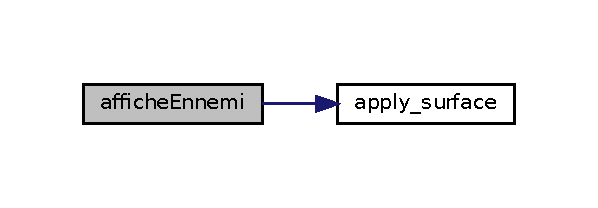
\includegraphics[width=272pt]{ennemies_8h_aeb2c0786744d55f91bc0dec00529aa7e_cgraph}
\end{center}
\end{figure}
Here is the caller graph for this function\+:
\nopagebreak
\begin{figure}[H]
\begin{center}
\leavevmode
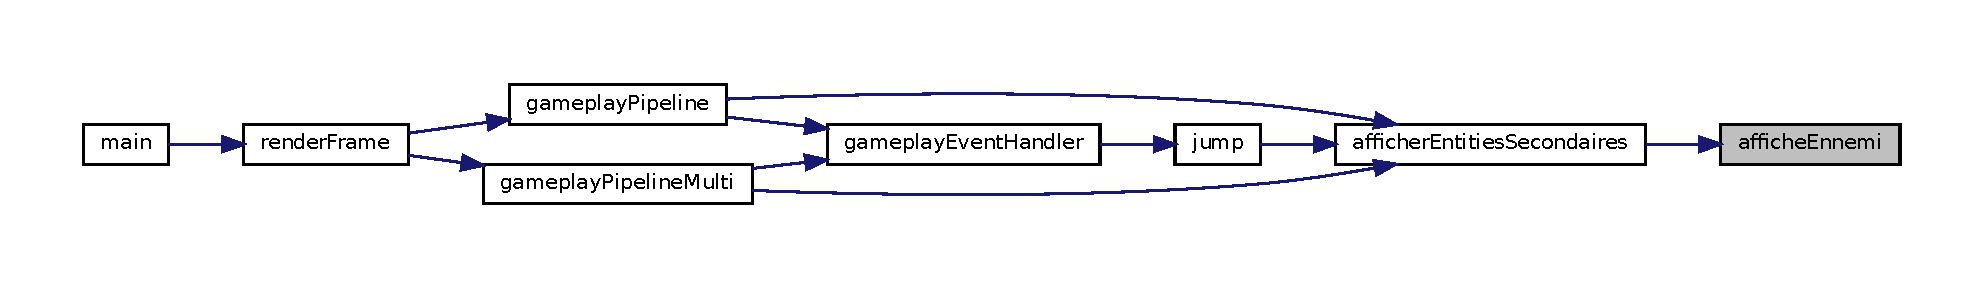
\includegraphics[width=350pt]{ennemies_8h_aeb2c0786744d55f91bc0dec00529aa7e_icgraph}
\end{center}
\end{figure}
\mbox{\Hypertarget{ennemies_8h_a6d3dff72d16d48b241a64beec64bec02}\label{ennemies_8h_a6d3dff72d16d48b241a64beec64bec02}} 
\index{ennemies.\+h@{ennemies.\+h}!init\+Ennemi@{init\+Ennemi}}
\index{init\+Ennemi@{init\+Ennemi}!ennemies.\+h@{ennemies.\+h}}
\subsubsection{\texorpdfstring{init\+Ennemi()}{initEnnemi()}}
{\footnotesize\ttfamily void init\+Ennemi (\begin{DoxyParamCaption}{ }\end{DoxyParamCaption})}

Here is the caller graph for this function\+:
\nopagebreak
\begin{figure}[H]
\begin{center}
\leavevmode
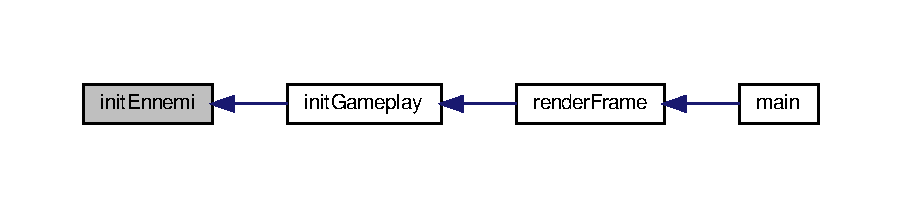
\includegraphics[width=350pt]{ennemies_8h_a6d3dff72d16d48b241a64beec64bec02_icgraph}
\end{center}
\end{figure}
\mbox{\Hypertarget{ennemies_8h_a67e4532e5a85ff89b0c393eb8cc7d614}\label{ennemies_8h_a67e4532e5a85ff89b0c393eb8cc7d614}} 
\index{ennemies.\+h@{ennemies.\+h}!kill\+Ennemy@{kill\+Ennemy}}
\index{kill\+Ennemy@{kill\+Ennemy}!ennemies.\+h@{ennemies.\+h}}
\subsubsection{\texorpdfstring{kill\+Ennemy()}{killEnnemy()}}
{\footnotesize\ttfamily \hyperlink{ennemies_8h_af688767ec0f4fdaa755e7f542c2d272d}{Ennemi} kill\+Ennemy (\begin{DoxyParamCaption}\item[{\hyperlink{ennemies_8h_af688767ec0f4fdaa755e7f542c2d272d}{Ennemi}}]{ennemi }\end{DoxyParamCaption})}

Here is the caller graph for this function\+:
\nopagebreak
\begin{figure}[H]
\begin{center}
\leavevmode
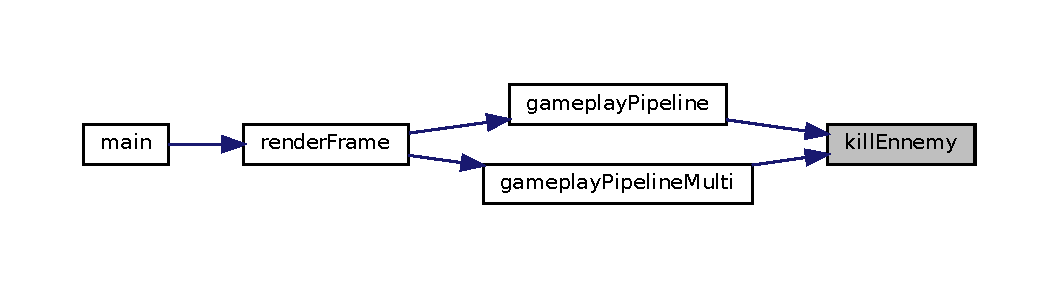
\includegraphics[width=350pt]{ennemies_8h_a67e4532e5a85ff89b0c393eb8cc7d614_icgraph}
\end{center}
\end{figure}
\mbox{\Hypertarget{ennemies_8h_aa135ada285717b081855f13fb28bc66d}\label{ennemies_8h_aa135ada285717b081855f13fb28bc66d}} 
\index{ennemies.\+h@{ennemies.\+h}!load\+Sprite\+Ennemi@{load\+Sprite\+Ennemi}}
\index{load\+Sprite\+Ennemi@{load\+Sprite\+Ennemi}!ennemies.\+h@{ennemies.\+h}}
\subsubsection{\texorpdfstring{load\+Sprite\+Ennemi()}{loadSpriteEnnemi()}}
{\footnotesize\ttfamily \hyperlink{ennemies_8h_af688767ec0f4fdaa755e7f542c2d272d}{Ennemi} load\+Sprite\+Ennemi (\begin{DoxyParamCaption}\item[{\hyperlink{ennemies_8h_af688767ec0f4fdaa755e7f542c2d272d}{Ennemi}}]{ennemi,  }\item[{int}]{direction }\end{DoxyParamCaption})}

Here is the call graph for this function\+:
\nopagebreak
\begin{figure}[H]
\begin{center}
\leavevmode
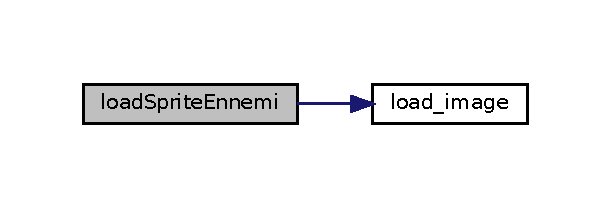
\includegraphics[width=275pt]{ennemies_8h_aa135ada285717b081855f13fb28bc66d_cgraph}
\end{center}
\end{figure}
Here is the caller graph for this function\+:
\nopagebreak
\begin{figure}[H]
\begin{center}
\leavevmode
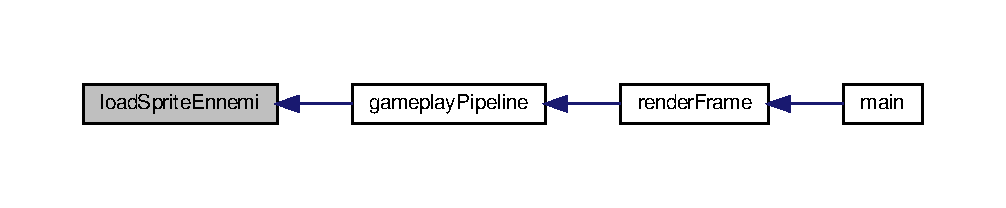
\includegraphics[width=350pt]{ennemies_8h_aa135ada285717b081855f13fb28bc66d_icgraph}
\end{center}
\end{figure}
\mbox{\Hypertarget{ennemies_8h_a3e7af8f799598c7440a820f5ba987187}\label{ennemies_8h_a3e7af8f799598c7440a820f5ba987187}} 
\index{ennemies.\+h@{ennemies.\+h}!remplir\+Tableau\+Ennemi@{remplir\+Tableau\+Ennemi}}
\index{remplir\+Tableau\+Ennemi@{remplir\+Tableau\+Ennemi}!ennemies.\+h@{ennemies.\+h}}
\subsubsection{\texorpdfstring{remplir\+Tableau\+Ennemi()}{remplirTableauEnnemi()}}
{\footnotesize\ttfamily void remplir\+Tableau\+Ennemi (\begin{DoxyParamCaption}{ }\end{DoxyParamCaption})}



\subsection{Variable Documentation}
\mbox{\Hypertarget{ennemies_8h_a3265575f87f7ec5947038321649ab4f2}\label{ennemies_8h_a3265575f87f7ec5947038321649ab4f2}} 
\index{ennemies.\+h@{ennemies.\+h}!ennemi1@{ennemi1}}
\index{ennemi1@{ennemi1}!ennemies.\+h@{ennemies.\+h}}
\subsubsection{\texorpdfstring{ennemi1}{ennemi1}}
{\footnotesize\ttfamily \hyperlink{ennemies_8h_af688767ec0f4fdaa755e7f542c2d272d}{Ennemi} ennemi1}

\mbox{\Hypertarget{ennemies_8h_a8b157a88dfbb24c7429fe2402dd445cd}\label{ennemies_8h_a8b157a88dfbb24c7429fe2402dd445cd}} 
\index{ennemies.\+h@{ennemies.\+h}!ennemi2@{ennemi2}}
\index{ennemi2@{ennemi2}!ennemies.\+h@{ennemies.\+h}}
\subsubsection{\texorpdfstring{ennemi2}{ennemi2}}
{\footnotesize\ttfamily \hyperlink{ennemies_8h_af688767ec0f4fdaa755e7f542c2d272d}{Ennemi} ennemi2}

\mbox{\Hypertarget{ennemies_8h_a141ba58c74a730d20dd02bcd067daf0a}\label{ennemies_8h_a141ba58c74a730d20dd02bcd067daf0a}} 
\index{ennemies.\+h@{ennemies.\+h}!ennemis@{ennemis}}
\index{ennemis@{ennemis}!ennemies.\+h@{ennemies.\+h}}
\subsubsection{\texorpdfstring{ennemis}{ennemis}}
{\footnotesize\ttfamily \hyperlink{ennemies_8h_af688767ec0f4fdaa755e7f542c2d272d}{Ennemi} ennemis\mbox{[}2\mbox{]}}


\hypertarget{gameplay_8c}{}\doxysection{gameplay.\+c File Reference}
\label{gameplay_8c}\index{gameplay.c@{gameplay.c}}


in-\/game gameplay source code  


{\ttfamily \#include \char`\"{}gameplay.\+h\char`\"{}}\newline
Include dependency graph for gameplay.\+c\+:\nopagebreak
\begin{figure}[H]
\begin{center}
\leavevmode
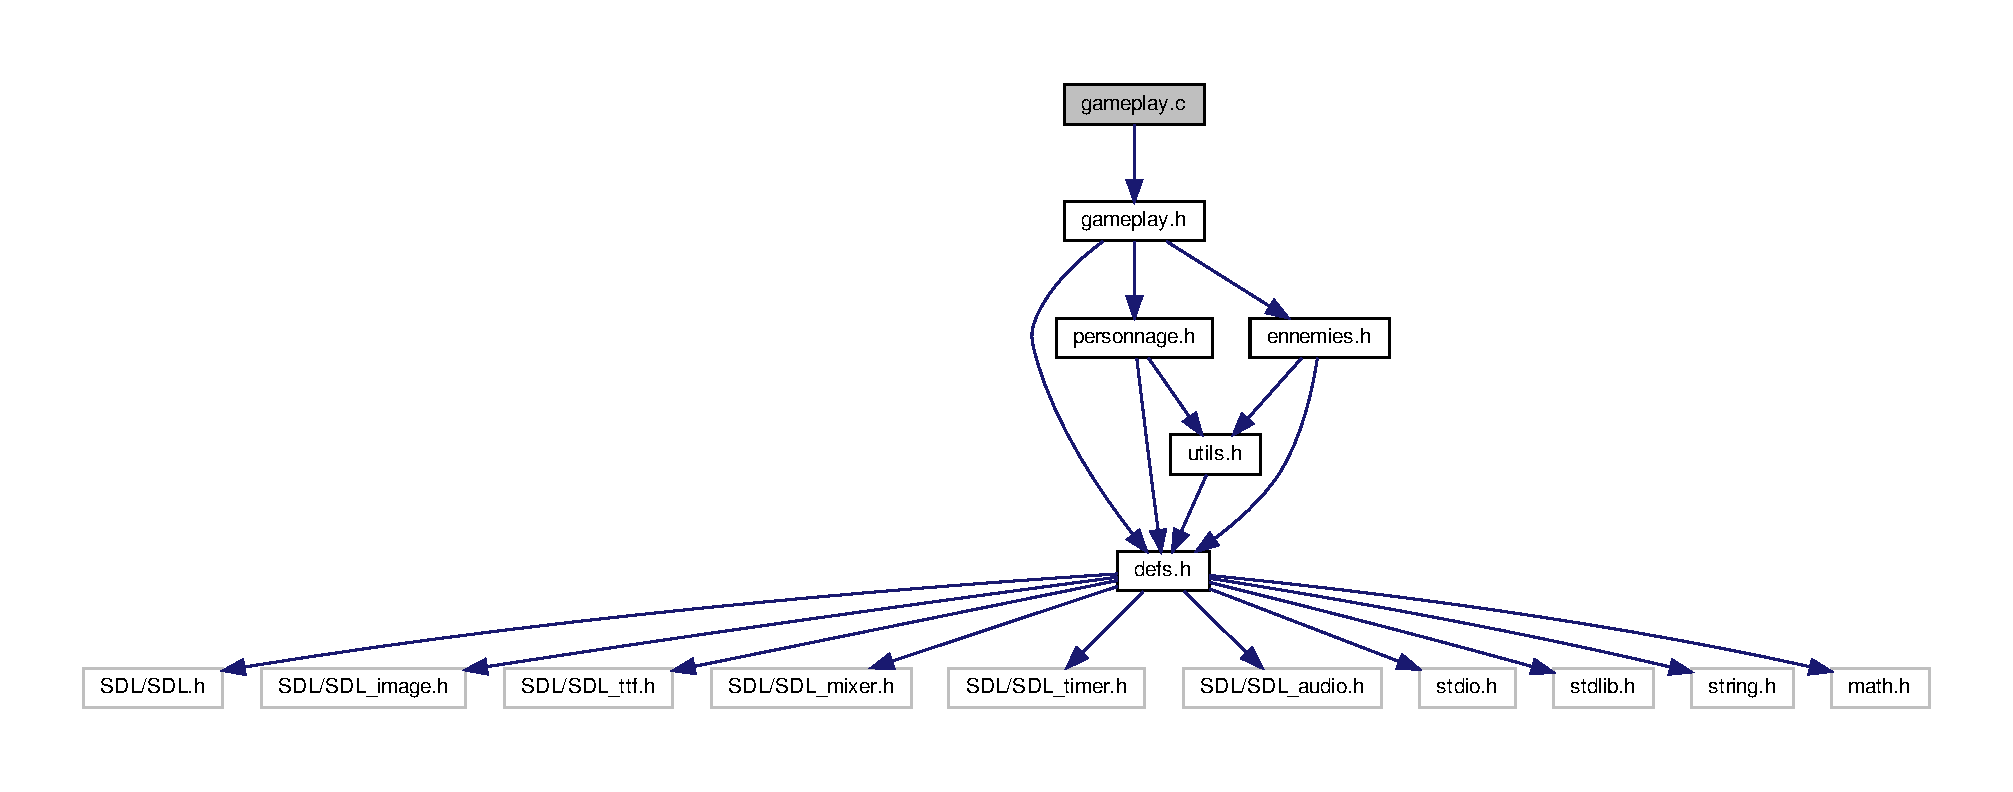
\includegraphics[width=350pt]{gameplay_8c__incl}
\end{center}
\end{figure}
\doxysubsection*{Functions}
\begin{DoxyCompactItemize}
\item 
\mbox{\hyperlink{personnage_8h_aae0cebaa519806b8e6c577443317f7c4}{Personnage}} \mbox{\hyperlink{gameplay_8c_a012cc3152aaa6256d7016eda4576e3e1}{jump}} (\mbox{\hyperlink{personnage_8h_aae0cebaa519806b8e6c577443317f7c4}{Personnage}} \mbox{\hyperlink{structpersonnage}{personnage}})
\item 
void \mbox{\hyperlink{gameplay_8c_ab12073167d36c929c41b6cf0862ab342}{load\+Vars}} ()
\item 
void \mbox{\hyperlink{gameplay_8c_a4acf497b379b922113b92fbc7846f6cc}{Save\+Vars}} ()
\item 
void \mbox{\hyperlink{gameplay_8c_ac9fb5524a1af1a6a5f5e62aed8e2aec2}{afficher\+Personnage}} (\mbox{\hyperlink{personnage_8h_aae0cebaa519806b8e6c577443317f7c4}{Personnage}} \mbox{\hyperlink{structpersonnage}{personnage}}, S\+D\+L\+\_\+\+Surface $\ast$\mbox{\hyperlink{defs_8h_a78fa3957d73de49cb81d047857504218}{screen}})
\item 
void \mbox{\hyperlink{gameplay_8c_aa3ab2db1ce3de55f90421f28085dfaa0}{init\+Gameplay}} ()
\item 
\mbox{\hyperlink{personnage_8h_aae0cebaa519806b8e6c577443317f7c4}{Personnage}} \mbox{\hyperlink{gameplay_8c_a19d24c21fe97bb7e71860600f57692c0}{gameplay\+Event\+Handler}} (\mbox{\hyperlink{personnage_8h_aae0cebaa519806b8e6c577443317f7c4}{Personnage}} \mbox{\hyperlink{structpersonnage}{personnage}})
\item 
void \mbox{\hyperlink{gameplay_8c_af5d079532bfd9c1e16366b419fd9b81c}{move\+Ennemies}} ()
\item 
void \mbox{\hyperlink{gameplay_8c_a1b0a0f001ccd6cbe4c186b9d6ea7a9a7}{afficher\+Entities\+Secondaires}} ()
\item 
int \mbox{\hyperlink{gameplay_8c_a2feec1d542e8b5cd6d712de11cbb3e20}{bounding\+Box\+Collision}} (S\+D\+L\+\_\+\+Rect A, S\+D\+L\+\_\+\+Rect B)
\item 
int \mbox{\hyperlink{gameplay_8c_a35ea5988cc7898b2c33b60749e31dbbf}{collision\+Detection}} (\mbox{\hyperlink{personnage_8h_aae0cebaa519806b8e6c577443317f7c4}{Personnage}} \mbox{\hyperlink{structpersonnage}{personnage}})
\item 
int \mbox{\hyperlink{gameplay_8c_acb81255bb5e5e4902254dc8f54ff20ab}{perfect\+Pixel\+Collision}} (\mbox{\hyperlink{personnage_8h_aae0cebaa519806b8e6c577443317f7c4}{Personnage}} \mbox{\hyperlink{structpersonnage}{personnage}}, int x, int y)
\item 
int \mbox{\hyperlink{gameplay_8c_a9b7cf0f7c2443726f0b4bb6012c09dda}{ennemy\+Vision}} (\mbox{\hyperlink{ennemies_8h_abc1d765bf177d92e054b9d9300b3ccef}{Ennemi}} \mbox{\hyperlink{structennemi}{ennemi}})
\item 
void \mbox{\hyperlink{gameplay_8c_a724ec64eedf57914a022a604b0251bba}{move\+Seen\+Ennemies}} ()
\item 
void \mbox{\hyperlink{gameplay_8c_aa4bbed40276a5850dab617b6e320a2dc}{show\+Game\+Over\+Screen}} ()
\item 
void \mbox{\hyperlink{gameplay_8c_a51e5ed834efb6cf170a430f12d1a234b}{show\+Minimap}} ()
\item 
void \mbox{\hyperlink{gameplay_8c_a22c68820a323b39d7ccb0b9f08ca8b06}{ai\+Move}} ()
\item 
void \mbox{\hyperlink{gameplay_8c_aceb86c980514c6c76f3e4f557c94560e}{gameplay\+Pipeline\+Multi}} ()
\item 
void \mbox{\hyperlink{gameplay_8c_a53f6e90f75c04f6d7214ef60dfdf9dee}{gameplay\+Pipeline}} ()
\end{DoxyCompactItemize}
\doxysubsection*{Variables}
\begin{DoxyCompactItemize}
\item 
\mbox{\hyperlink{personnage_8h_aae0cebaa519806b8e6c577443317f7c4}{Personnage}} \mbox{\hyperlink{gameplay_8c_abd0321820747a312cdec82d73f26f9fa}{personnage}}
\item 
\mbox{\hyperlink{personnage_8h_aae0cebaa519806b8e6c577443317f7c4}{Personnage}} \mbox{\hyperlink{gameplay_8c_a1175b0457a2ae93a8ee11f07f199f66e}{personnage2}}
\end{DoxyCompactItemize}


\doxysubsection{Detailed Description}
in-\/game gameplay source code 

\begin{DoxyAuthor}{Author}
Creative Sparks 
\end{DoxyAuthor}
\begin{DoxyVersion}{Version}
2.\+0 
\end{DoxyVersion}
\begin{DoxyDate}{Date}
2020 
\end{DoxyDate}


\doxysubsection{Function Documentation}
\mbox{\Hypertarget{gameplay_8c_a1b0a0f001ccd6cbe4c186b9d6ea7a9a7}\label{gameplay_8c_a1b0a0f001ccd6cbe4c186b9d6ea7a9a7}} 
\index{gameplay.c@{gameplay.c}!afficherEntitiesSecondaires@{afficherEntitiesSecondaires}}
\index{afficherEntitiesSecondaires@{afficherEntitiesSecondaires}!gameplay.c@{gameplay.c}}
\doxysubsubsection{\texorpdfstring{afficherEntitiesSecondaires()}{afficherEntitiesSecondaires()}}
{\footnotesize\ttfamily void afficher\+Entities\+Secondaires (\begin{DoxyParamCaption}{ }\end{DoxyParamCaption})}

Here is the call graph for this function\+:\nopagebreak
\begin{figure}[H]
\begin{center}
\leavevmode
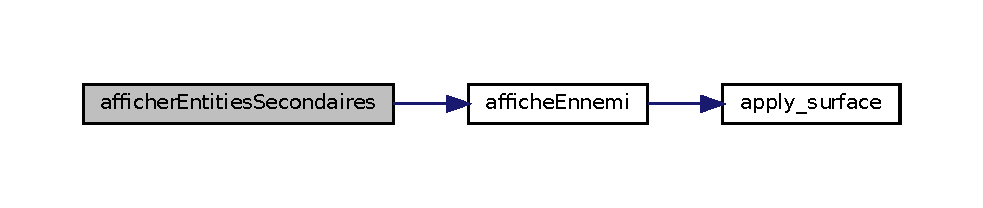
\includegraphics[width=350pt]{gameplay_8c_a1b0a0f001ccd6cbe4c186b9d6ea7a9a7_cgraph}
\end{center}
\end{figure}
Here is the caller graph for this function\+:\nopagebreak
\begin{figure}[H]
\begin{center}
\leavevmode
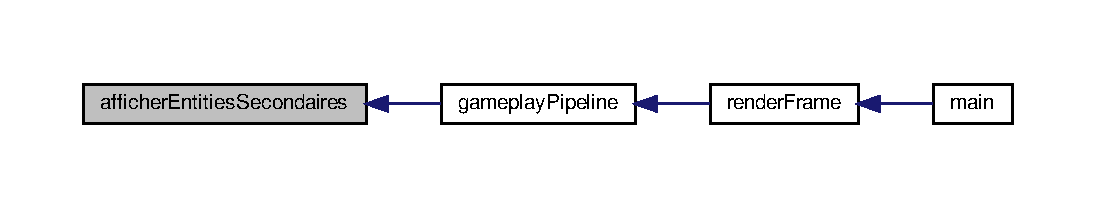
\includegraphics[width=350pt]{gameplay_8c_a1b0a0f001ccd6cbe4c186b9d6ea7a9a7_icgraph}
\end{center}
\end{figure}
\mbox{\Hypertarget{gameplay_8c_ac9fb5524a1af1a6a5f5e62aed8e2aec2}\label{gameplay_8c_ac9fb5524a1af1a6a5f5e62aed8e2aec2}} 
\index{gameplay.c@{gameplay.c}!afficherPersonnage@{afficherPersonnage}}
\index{afficherPersonnage@{afficherPersonnage}!gameplay.c@{gameplay.c}}
\doxysubsubsection{\texorpdfstring{afficherPersonnage()}{afficherPersonnage()}}
{\footnotesize\ttfamily void afficher\+Personnage (\begin{DoxyParamCaption}\item[{\mbox{\hyperlink{personnage_8h_aae0cebaa519806b8e6c577443317f7c4}{Personnage}}}]{personnage,  }\item[{S\+D\+L\+\_\+\+Surface $\ast$}]{screen }\end{DoxyParamCaption})}

Here is the call graph for this function\+:\nopagebreak
\begin{figure}[H]
\begin{center}
\leavevmode
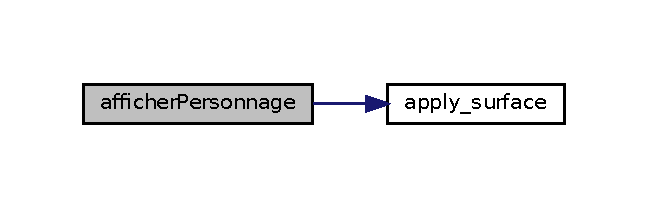
\includegraphics[width=311pt]{gameplay_8c_ac9fb5524a1af1a6a5f5e62aed8e2aec2_cgraph}
\end{center}
\end{figure}
\mbox{\Hypertarget{gameplay_8c_a22c68820a323b39d7ccb0b9f08ca8b06}\label{gameplay_8c_a22c68820a323b39d7ccb0b9f08ca8b06}} 
\index{gameplay.c@{gameplay.c}!aiMove@{aiMove}}
\index{aiMove@{aiMove}!gameplay.c@{gameplay.c}}
\doxysubsubsection{\texorpdfstring{aiMove()}{aiMove()}}
{\footnotesize\ttfamily void ai\+Move (\begin{DoxyParamCaption}{ }\end{DoxyParamCaption})}

Here is the caller graph for this function\+:\nopagebreak
\begin{figure}[H]
\begin{center}
\leavevmode
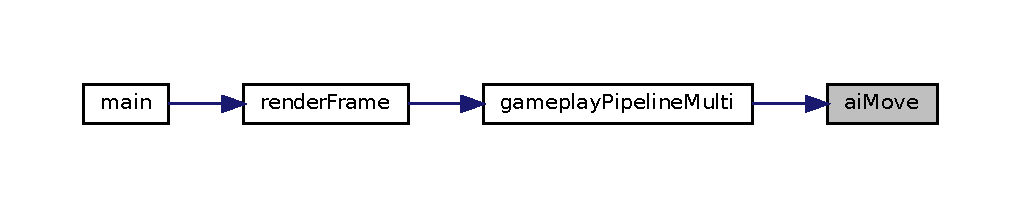
\includegraphics[width=350pt]{gameplay_8c_a22c68820a323b39d7ccb0b9f08ca8b06_icgraph}
\end{center}
\end{figure}
\mbox{\Hypertarget{gameplay_8c_a2feec1d542e8b5cd6d712de11cbb3e20}\label{gameplay_8c_a2feec1d542e8b5cd6d712de11cbb3e20}} 
\index{gameplay.c@{gameplay.c}!boundingBoxCollision@{boundingBoxCollision}}
\index{boundingBoxCollision@{boundingBoxCollision}!gameplay.c@{gameplay.c}}
\doxysubsubsection{\texorpdfstring{boundingBoxCollision()}{boundingBoxCollision()}}
{\footnotesize\ttfamily int bounding\+Box\+Collision (\begin{DoxyParamCaption}\item[{S\+D\+L\+\_\+\+Rect}]{A,  }\item[{S\+D\+L\+\_\+\+Rect}]{B }\end{DoxyParamCaption})}

Here is the caller graph for this function\+:\nopagebreak
\begin{figure}[H]
\begin{center}
\leavevmode
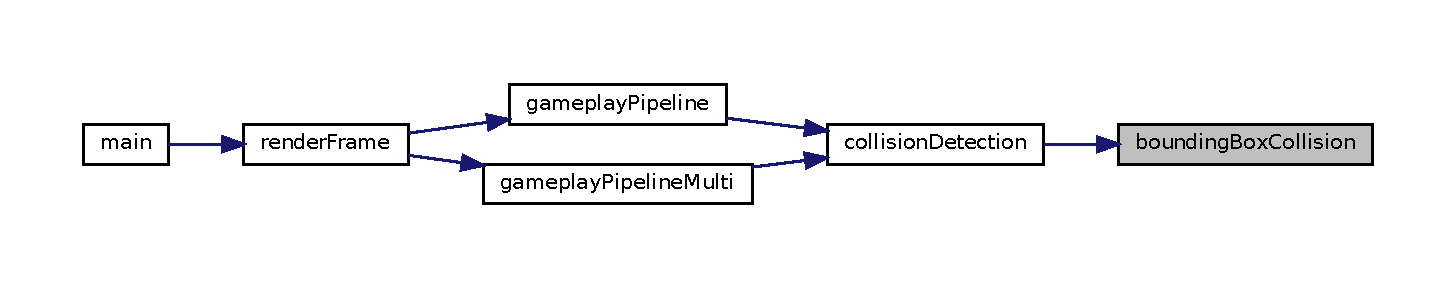
\includegraphics[width=350pt]{gameplay_8c_a2feec1d542e8b5cd6d712de11cbb3e20_icgraph}
\end{center}
\end{figure}
\mbox{\Hypertarget{gameplay_8c_a35ea5988cc7898b2c33b60749e31dbbf}\label{gameplay_8c_a35ea5988cc7898b2c33b60749e31dbbf}} 
\index{gameplay.c@{gameplay.c}!collisionDetection@{collisionDetection}}
\index{collisionDetection@{collisionDetection}!gameplay.c@{gameplay.c}}
\doxysubsubsection{\texorpdfstring{collisionDetection()}{collisionDetection()}}
{\footnotesize\ttfamily int collision\+Detection (\begin{DoxyParamCaption}\item[{\mbox{\hyperlink{personnage_8h_aae0cebaa519806b8e6c577443317f7c4}{Personnage}}}]{personnage }\end{DoxyParamCaption})}

Here is the call graph for this function\+:\nopagebreak
\begin{figure}[H]
\begin{center}
\leavevmode
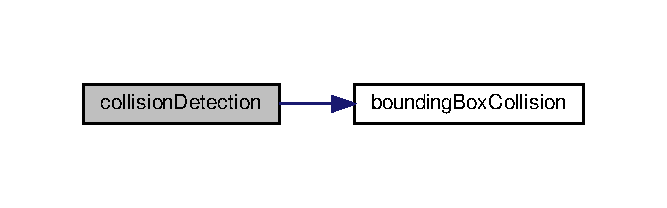
\includegraphics[width=342pt]{gameplay_8c_a35ea5988cc7898b2c33b60749e31dbbf_cgraph}
\end{center}
\end{figure}
Here is the caller graph for this function\+:\nopagebreak
\begin{figure}[H]
\begin{center}
\leavevmode
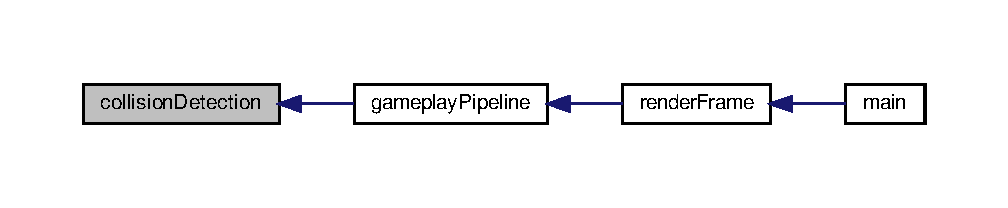
\includegraphics[width=350pt]{gameplay_8c_a35ea5988cc7898b2c33b60749e31dbbf_icgraph}
\end{center}
\end{figure}
\mbox{\Hypertarget{gameplay_8c_a9b7cf0f7c2443726f0b4bb6012c09dda}\label{gameplay_8c_a9b7cf0f7c2443726f0b4bb6012c09dda}} 
\index{gameplay.c@{gameplay.c}!ennemyVision@{ennemyVision}}
\index{ennemyVision@{ennemyVision}!gameplay.c@{gameplay.c}}
\doxysubsubsection{\texorpdfstring{ennemyVision()}{ennemyVision()}}
{\footnotesize\ttfamily int ennemy\+Vision (\begin{DoxyParamCaption}\item[{\mbox{\hyperlink{ennemies_8h_abc1d765bf177d92e054b9d9300b3ccef}{Ennemi}}}]{ennemi }\end{DoxyParamCaption})}

Here is the caller graph for this function\+:\nopagebreak
\begin{figure}[H]
\begin{center}
\leavevmode
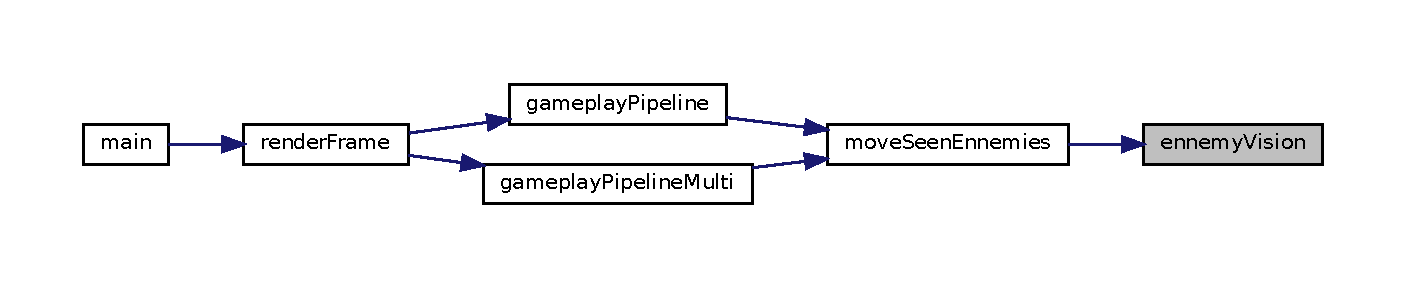
\includegraphics[width=350pt]{gameplay_8c_a9b7cf0f7c2443726f0b4bb6012c09dda_icgraph}
\end{center}
\end{figure}
\mbox{\Hypertarget{gameplay_8c_a19d24c21fe97bb7e71860600f57692c0}\label{gameplay_8c_a19d24c21fe97bb7e71860600f57692c0}} 
\index{gameplay.c@{gameplay.c}!gameplayEventHandler@{gameplayEventHandler}}
\index{gameplayEventHandler@{gameplayEventHandler}!gameplay.c@{gameplay.c}}
\doxysubsubsection{\texorpdfstring{gameplayEventHandler()}{gameplayEventHandler()}}
{\footnotesize\ttfamily \mbox{\hyperlink{personnage_8h_aae0cebaa519806b8e6c577443317f7c4}{Personnage}} gameplay\+Event\+Handler (\begin{DoxyParamCaption}\item[{\mbox{\hyperlink{personnage_8h_aae0cebaa519806b8e6c577443317f7c4}{Personnage}}}]{personnage }\end{DoxyParamCaption})}

Here is the call graph for this function\+:\nopagebreak
\begin{figure}[H]
\begin{center}
\leavevmode
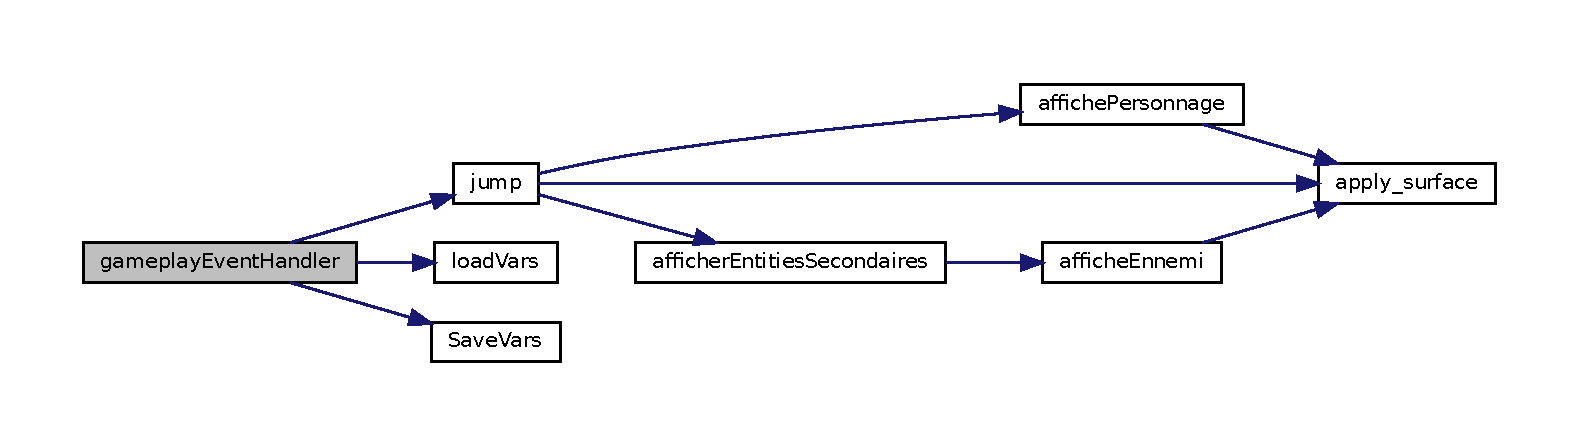
\includegraphics[width=350pt]{gameplay_8c_a19d24c21fe97bb7e71860600f57692c0_cgraph}
\end{center}
\end{figure}
Here is the caller graph for this function\+:\nopagebreak
\begin{figure}[H]
\begin{center}
\leavevmode
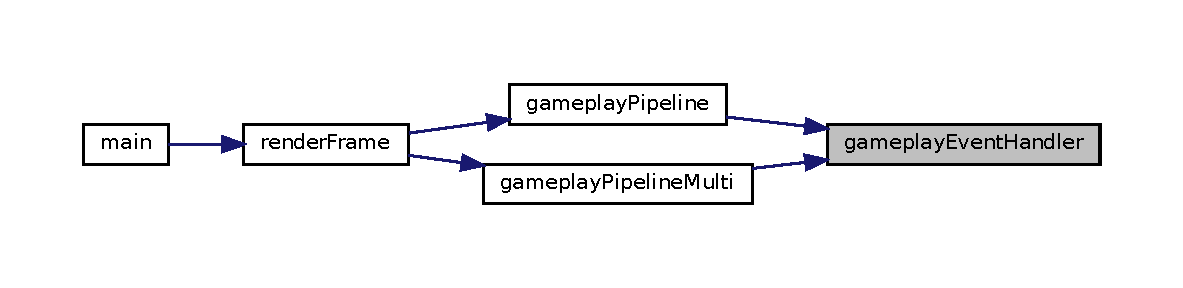
\includegraphics[width=350pt]{gameplay_8c_a19d24c21fe97bb7e71860600f57692c0_icgraph}
\end{center}
\end{figure}
\mbox{\Hypertarget{gameplay_8c_a53f6e90f75c04f6d7214ef60dfdf9dee}\label{gameplay_8c_a53f6e90f75c04f6d7214ef60dfdf9dee}} 
\index{gameplay.c@{gameplay.c}!gameplayPipeline@{gameplayPipeline}}
\index{gameplayPipeline@{gameplayPipeline}!gameplay.c@{gameplay.c}}
\doxysubsubsection{\texorpdfstring{gameplayPipeline()}{gameplayPipeline()}}
{\footnotesize\ttfamily void gameplay\+Pipeline (\begin{DoxyParamCaption}{ }\end{DoxyParamCaption})}

Here is the call graph for this function\+:\nopagebreak
\begin{figure}[H]
\begin{center}
\leavevmode
\includegraphics[width=350pt]{gameplay_8c_a53f6e90f75c04f6d7214ef60dfdf9dee_cgraph}
\end{center}
\end{figure}
Here is the caller graph for this function\+:\nopagebreak
\begin{figure}[H]
\begin{center}
\leavevmode
\includegraphics[width=350pt]{gameplay_8c_a53f6e90f75c04f6d7214ef60dfdf9dee_icgraph}
\end{center}
\end{figure}
\mbox{\Hypertarget{gameplay_8c_aceb86c980514c6c76f3e4f557c94560e}\label{gameplay_8c_aceb86c980514c6c76f3e4f557c94560e}} 
\index{gameplay.c@{gameplay.c}!gameplayPipelineMulti@{gameplayPipelineMulti}}
\index{gameplayPipelineMulti@{gameplayPipelineMulti}!gameplay.c@{gameplay.c}}
\doxysubsubsection{\texorpdfstring{gameplayPipelineMulti()}{gameplayPipelineMulti()}}
{\footnotesize\ttfamily void gameplay\+Pipeline\+Multi (\begin{DoxyParamCaption}{ }\end{DoxyParamCaption})}

Here is the call graph for this function\+:\nopagebreak
\begin{figure}[H]
\begin{center}
\leavevmode
\includegraphics[width=350pt]{gameplay_8c_aceb86c980514c6c76f3e4f557c94560e_cgraph}
\end{center}
\end{figure}
Here is the caller graph for this function\+:\nopagebreak
\begin{figure}[H]
\begin{center}
\leavevmode
\includegraphics[width=350pt]{gameplay_8c_aceb86c980514c6c76f3e4f557c94560e_icgraph}
\end{center}
\end{figure}
\mbox{\Hypertarget{gameplay_8c_aa3ab2db1ce3de55f90421f28085dfaa0}\label{gameplay_8c_aa3ab2db1ce3de55f90421f28085dfaa0}} 
\index{gameplay.c@{gameplay.c}!initGameplay@{initGameplay}}
\index{initGameplay@{initGameplay}!gameplay.c@{gameplay.c}}
\doxysubsubsection{\texorpdfstring{initGameplay()}{initGameplay()}}
{\footnotesize\ttfamily void init\+Gameplay (\begin{DoxyParamCaption}{ }\end{DoxyParamCaption})}

Here is the call graph for this function\+:\nopagebreak
\begin{figure}[H]
\begin{center}
\leavevmode
\includegraphics[width=294pt]{gameplay_8c_aa3ab2db1ce3de55f90421f28085dfaa0_cgraph}
\end{center}
\end{figure}
Here is the caller graph for this function\+:\nopagebreak
\begin{figure}[H]
\begin{center}
\leavevmode
\includegraphics[width=350pt]{gameplay_8c_aa3ab2db1ce3de55f90421f28085dfaa0_icgraph}
\end{center}
\end{figure}
\mbox{\Hypertarget{gameplay_8c_a012cc3152aaa6256d7016eda4576e3e1}\label{gameplay_8c_a012cc3152aaa6256d7016eda4576e3e1}} 
\index{gameplay.c@{gameplay.c}!jump@{jump}}
\index{jump@{jump}!gameplay.c@{gameplay.c}}
\doxysubsubsection{\texorpdfstring{jump()}{jump()}}
{\footnotesize\ttfamily \mbox{\hyperlink{personnage_8h_aae0cebaa519806b8e6c577443317f7c4}{Personnage}} jump (\begin{DoxyParamCaption}\item[{\mbox{\hyperlink{personnage_8h_aae0cebaa519806b8e6c577443317f7c4}{Personnage}}}]{personnage }\end{DoxyParamCaption})}

Here is the call graph for this function\+:\nopagebreak
\begin{figure}[H]
\begin{center}
\leavevmode
\includegraphics[width=350pt]{gameplay_8c_a012cc3152aaa6256d7016eda4576e3e1_cgraph}
\end{center}
\end{figure}
Here is the caller graph for this function\+:\nopagebreak
\begin{figure}[H]
\begin{center}
\leavevmode
\includegraphics[width=350pt]{gameplay_8c_a012cc3152aaa6256d7016eda4576e3e1_icgraph}
\end{center}
\end{figure}
\mbox{\Hypertarget{gameplay_8c_ab12073167d36c929c41b6cf0862ab342}\label{gameplay_8c_ab12073167d36c929c41b6cf0862ab342}} 
\index{gameplay.c@{gameplay.c}!loadVars@{loadVars}}
\index{loadVars@{loadVars}!gameplay.c@{gameplay.c}}
\doxysubsubsection{\texorpdfstring{loadVars()}{loadVars()}}
{\footnotesize\ttfamily void load\+Vars (\begin{DoxyParamCaption}{ }\end{DoxyParamCaption})}

Here is the caller graph for this function\+:\nopagebreak
\begin{figure}[H]
\begin{center}
\leavevmode
\includegraphics[width=350pt]{gameplay_8c_ab12073167d36c929c41b6cf0862ab342_icgraph}
\end{center}
\end{figure}
\mbox{\Hypertarget{gameplay_8c_af5d079532bfd9c1e16366b419fd9b81c}\label{gameplay_8c_af5d079532bfd9c1e16366b419fd9b81c}} 
\index{gameplay.c@{gameplay.c}!moveEnnemies@{moveEnnemies}}
\index{moveEnnemies@{moveEnnemies}!gameplay.c@{gameplay.c}}
\doxysubsubsection{\texorpdfstring{moveEnnemies()}{moveEnnemies()}}
{\footnotesize\ttfamily void move\+Ennemies (\begin{DoxyParamCaption}{ }\end{DoxyParamCaption})}

Here is the caller graph for this function\+:\nopagebreak
\begin{figure}[H]
\begin{center}
\leavevmode
\includegraphics[width=350pt]{gameplay_8c_af5d079532bfd9c1e16366b419fd9b81c_icgraph}
\end{center}
\end{figure}
\mbox{\Hypertarget{gameplay_8c_a724ec64eedf57914a022a604b0251bba}\label{gameplay_8c_a724ec64eedf57914a022a604b0251bba}} 
\index{gameplay.c@{gameplay.c}!moveSeenEnnemies@{moveSeenEnnemies}}
\index{moveSeenEnnemies@{moveSeenEnnemies}!gameplay.c@{gameplay.c}}
\doxysubsubsection{\texorpdfstring{moveSeenEnnemies()}{moveSeenEnnemies()}}
{\footnotesize\ttfamily void move\+Seen\+Ennemies (\begin{DoxyParamCaption}{ }\end{DoxyParamCaption})}

Here is the call graph for this function\+:\nopagebreak
\begin{figure}[H]
\begin{center}
\leavevmode
\includegraphics[width=318pt]{gameplay_8c_a724ec64eedf57914a022a604b0251bba_cgraph}
\end{center}
\end{figure}
Here is the caller graph for this function\+:\nopagebreak
\begin{figure}[H]
\begin{center}
\leavevmode
\includegraphics[width=350pt]{gameplay_8c_a724ec64eedf57914a022a604b0251bba_icgraph}
\end{center}
\end{figure}
\mbox{\Hypertarget{gameplay_8c_acb81255bb5e5e4902254dc8f54ff20ab}\label{gameplay_8c_acb81255bb5e5e4902254dc8f54ff20ab}} 
\index{gameplay.c@{gameplay.c}!perfectPixelCollision@{perfectPixelCollision}}
\index{perfectPixelCollision@{perfectPixelCollision}!gameplay.c@{gameplay.c}}
\doxysubsubsection{\texorpdfstring{perfectPixelCollision()}{perfectPixelCollision()}}
{\footnotesize\ttfamily int perfect\+Pixel\+Collision (\begin{DoxyParamCaption}\item[{\mbox{\hyperlink{personnage_8h_aae0cebaa519806b8e6c577443317f7c4}{Personnage}}}]{personnage,  }\item[{int}]{x,  }\item[{int}]{y }\end{DoxyParamCaption})}

Here is the call graph for this function\+:\nopagebreak
\begin{figure}[H]
\begin{center}
\leavevmode
\includegraphics[width=289pt]{gameplay_8c_acb81255bb5e5e4902254dc8f54ff20ab_cgraph}
\end{center}
\end{figure}
\mbox{\Hypertarget{gameplay_8c_a4acf497b379b922113b92fbc7846f6cc}\label{gameplay_8c_a4acf497b379b922113b92fbc7846f6cc}} 
\index{gameplay.c@{gameplay.c}!SaveVars@{SaveVars}}
\index{SaveVars@{SaveVars}!gameplay.c@{gameplay.c}}
\doxysubsubsection{\texorpdfstring{SaveVars()}{SaveVars()}}
{\footnotesize\ttfamily void Save\+Vars (\begin{DoxyParamCaption}{ }\end{DoxyParamCaption})}

Here is the caller graph for this function\+:\nopagebreak
\begin{figure}[H]
\begin{center}
\leavevmode
\includegraphics[width=350pt]{gameplay_8c_a4acf497b379b922113b92fbc7846f6cc_icgraph}
\end{center}
\end{figure}
\mbox{\Hypertarget{gameplay_8c_aa4bbed40276a5850dab617b6e320a2dc}\label{gameplay_8c_aa4bbed40276a5850dab617b6e320a2dc}} 
\index{gameplay.c@{gameplay.c}!showGameOverScreen@{showGameOverScreen}}
\index{showGameOverScreen@{showGameOverScreen}!gameplay.c@{gameplay.c}}
\doxysubsubsection{\texorpdfstring{showGameOverScreen()}{showGameOverScreen()}}
{\footnotesize\ttfamily void show\+Game\+Over\+Screen (\begin{DoxyParamCaption}{ }\end{DoxyParamCaption})}

Here is the call graph for this function\+:\nopagebreak
\begin{figure}[H]
\begin{center}
\leavevmode
\includegraphics[width=350pt]{gameplay_8c_aa4bbed40276a5850dab617b6e320a2dc_cgraph}
\end{center}
\end{figure}
Here is the caller graph for this function\+:\nopagebreak
\begin{figure}[H]
\begin{center}
\leavevmode
\includegraphics[width=350pt]{gameplay_8c_aa4bbed40276a5850dab617b6e320a2dc_icgraph}
\end{center}
\end{figure}
\mbox{\Hypertarget{gameplay_8c_a51e5ed834efb6cf170a430f12d1a234b}\label{gameplay_8c_a51e5ed834efb6cf170a430f12d1a234b}} 
\index{gameplay.c@{gameplay.c}!showMinimap@{showMinimap}}
\index{showMinimap@{showMinimap}!gameplay.c@{gameplay.c}}
\doxysubsubsection{\texorpdfstring{showMinimap()}{showMinimap()}}
{\footnotesize\ttfamily void show\+Minimap (\begin{DoxyParamCaption}{ }\end{DoxyParamCaption})}



\doxysubsection{Variable Documentation}
\mbox{\Hypertarget{gameplay_8c_abd0321820747a312cdec82d73f26f9fa}\label{gameplay_8c_abd0321820747a312cdec82d73f26f9fa}} 
\index{gameplay.c@{gameplay.c}!personnage@{personnage}}
\index{personnage@{personnage}!gameplay.c@{gameplay.c}}
\doxysubsubsection{\texorpdfstring{personnage}{personnage}}
{\footnotesize\ttfamily \mbox{\hyperlink{personnage_8h_aae0cebaa519806b8e6c577443317f7c4}{Personnage}} \mbox{\hyperlink{structpersonnage}{personnage}}}

\mbox{\Hypertarget{gameplay_8c_a1175b0457a2ae93a8ee11f07f199f66e}\label{gameplay_8c_a1175b0457a2ae93a8ee11f07f199f66e}} 
\index{gameplay.c@{gameplay.c}!personnage2@{personnage2}}
\index{personnage2@{personnage2}!gameplay.c@{gameplay.c}}
\doxysubsubsection{\texorpdfstring{personnage2}{personnage2}}
{\footnotesize\ttfamily \mbox{\hyperlink{personnage_8h_aae0cebaa519806b8e6c577443317f7c4}{Personnage}} personnage2}


\hypertarget{gameplay_8h}{}\doxysection{gameplay.\+h File Reference}
\label{gameplay_8h}\index{gameplay.h@{gameplay.h}}


in-\/game function prototypes  


{\ttfamily \#include \char`\"{}defs.\+h\char`\"{}}\newline
{\ttfamily \#include \char`\"{}personnage.\+h\char`\"{}}\newline
{\ttfamily \#include \char`\"{}ennemies.\+h\char`\"{}}\newline
Include dependency graph for gameplay.\+h\+:\nopagebreak
\begin{figure}[H]
\begin{center}
\leavevmode
\includegraphics[width=350pt]{gameplay_8h__incl}
\end{center}
\end{figure}
This graph shows which files directly or indirectly include this file\+:\nopagebreak
\begin{figure}[H]
\begin{center}
\leavevmode
\includegraphics[width=216pt]{gameplay_8h__dep__incl}
\end{center}
\end{figure}
\doxysubsection*{Data Structures}
\begin{DoxyCompactItemize}
\item 
struct \mbox{\hyperlink{structsaveFile}{save\+File}}
\begin{DoxyCompactList}\small\item\em struct for file Saving \end{DoxyCompactList}\end{DoxyCompactItemize}
\doxysubsection*{Typedefs}
\begin{DoxyCompactItemize}
\item 
typedef struct \mbox{\hyperlink{structsaveFile}{save\+File}} \mbox{\hyperlink{gameplay_8h_ae314d5f010add0eb47950cd6548733ea}{Save\+File}}
\end{DoxyCompactItemize}
\doxysubsection*{Functions}
\begin{DoxyCompactItemize}
\item 
void \mbox{\hyperlink{gameplay_8h_ac9fb5524a1af1a6a5f5e62aed8e2aec2}{afficher\+Personnage}} (\mbox{\hyperlink{personnage_8h_aae0cebaa519806b8e6c577443317f7c4}{Personnage}} \mbox{\hyperlink{structpersonnage}{personnage}}, S\+D\+L\+\_\+\+Surface $\ast$\mbox{\hyperlink{defs_8h_a78fa3957d73de49cb81d047857504218}{screen}})
\item 
void \mbox{\hyperlink{gameplay_8h_a1b0a0f001ccd6cbe4c186b9d6ea7a9a7}{afficher\+Entities\+Secondaires}} ()
\item 
int \mbox{\hyperlink{gameplay_8h_a35ea5988cc7898b2c33b60749e31dbbf}{collision\+Detection}} (\mbox{\hyperlink{personnage_8h_aae0cebaa519806b8e6c577443317f7c4}{Personnage}} \mbox{\hyperlink{structpersonnage}{personnage}})
\item 
int \mbox{\hyperlink{gameplay_8h_afe07e215da3410208176e3f9c0988694}{bounding\+Box\+Collision}} (S\+D\+L\+\_\+\+Rect a, S\+D\+L\+\_\+\+Rect b)
\item 
int \mbox{\hyperlink{gameplay_8h_acb81255bb5e5e4902254dc8f54ff20ab}{perfect\+Pixel\+Collision}} (\mbox{\hyperlink{personnage_8h_aae0cebaa519806b8e6c577443317f7c4}{Personnage}} \mbox{\hyperlink{structpersonnage}{personnage}}, int x, int y)
\item 
void \mbox{\hyperlink{gameplay_8h_aa3ab2db1ce3de55f90421f28085dfaa0}{init\+Gameplay}} ()
\item 
void \mbox{\hyperlink{gameplay_8h_af5d079532bfd9c1e16366b419fd9b81c}{move\+Ennemies}} ()
\item 
void \mbox{\hyperlink{gameplay_8h_a53f6e90f75c04f6d7214ef60dfdf9dee}{gameplay\+Pipeline}} ()
\item 
void \mbox{\hyperlink{gameplay_8h_aceb86c980514c6c76f3e4f557c94560e}{gameplay\+Pipeline\+Multi}} ()
\item 
int \mbox{\hyperlink{gameplay_8h_a9b7cf0f7c2443726f0b4bb6012c09dda}{ennemy\+Vision}} (\mbox{\hyperlink{ennemies_8h_abc1d765bf177d92e054b9d9300b3ccef}{Ennemi}} \mbox{\hyperlink{structennemi}{ennemi}})
\item 
void \mbox{\hyperlink{gameplay_8h_ab12073167d36c929c41b6cf0862ab342}{load\+Vars}} ()
\item 
void \mbox{\hyperlink{gameplay_8h_a4acf497b379b922113b92fbc7846f6cc}{Save\+Vars}} ()
\end{DoxyCompactItemize}


\doxysubsection{Detailed Description}
in-\/game function prototypes 

\begin{DoxyAuthor}{Author}
Creative Sparks 
\end{DoxyAuthor}
\begin{DoxyVersion}{Version}
2.\+0 
\end{DoxyVersion}
\begin{DoxyDate}{Date}
2020 
\end{DoxyDate}


\doxysubsection{Typedef Documentation}
\mbox{\Hypertarget{gameplay_8h_ae314d5f010add0eb47950cd6548733ea}\label{gameplay_8h_ae314d5f010add0eb47950cd6548733ea}} 
\index{gameplay.h@{gameplay.h}!SaveFile@{SaveFile}}
\index{SaveFile@{SaveFile}!gameplay.h@{gameplay.h}}
\doxysubsubsection{\texorpdfstring{SaveFile}{SaveFile}}
{\footnotesize\ttfamily typedef struct \mbox{\hyperlink{structsaveFile}{save\+File}} \mbox{\hyperlink{gameplay_8h_ae314d5f010add0eb47950cd6548733ea}{Save\+File}}}



\doxysubsection{Function Documentation}
\mbox{\Hypertarget{gameplay_8h_a1b0a0f001ccd6cbe4c186b9d6ea7a9a7}\label{gameplay_8h_a1b0a0f001ccd6cbe4c186b9d6ea7a9a7}} 
\index{gameplay.h@{gameplay.h}!afficherEntitiesSecondaires@{afficherEntitiesSecondaires}}
\index{afficherEntitiesSecondaires@{afficherEntitiesSecondaires}!gameplay.h@{gameplay.h}}
\doxysubsubsection{\texorpdfstring{afficherEntitiesSecondaires()}{afficherEntitiesSecondaires()}}
{\footnotesize\ttfamily void afficher\+Entities\+Secondaires (\begin{DoxyParamCaption}{ }\end{DoxyParamCaption})}

Here is the call graph for this function\+:\nopagebreak
\begin{figure}[H]
\begin{center}
\leavevmode
\includegraphics[width=350pt]{gameplay_8h_a1b0a0f001ccd6cbe4c186b9d6ea7a9a7_cgraph}
\end{center}
\end{figure}
Here is the caller graph for this function\+:\nopagebreak
\begin{figure}[H]
\begin{center}
\leavevmode
\includegraphics[width=350pt]{gameplay_8h_a1b0a0f001ccd6cbe4c186b9d6ea7a9a7_icgraph}
\end{center}
\end{figure}
\mbox{\Hypertarget{gameplay_8h_ac9fb5524a1af1a6a5f5e62aed8e2aec2}\label{gameplay_8h_ac9fb5524a1af1a6a5f5e62aed8e2aec2}} 
\index{gameplay.h@{gameplay.h}!afficherPersonnage@{afficherPersonnage}}
\index{afficherPersonnage@{afficherPersonnage}!gameplay.h@{gameplay.h}}
\doxysubsubsection{\texorpdfstring{afficherPersonnage()}{afficherPersonnage()}}
{\footnotesize\ttfamily void afficher\+Personnage (\begin{DoxyParamCaption}\item[{\mbox{\hyperlink{personnage_8h_aae0cebaa519806b8e6c577443317f7c4}{Personnage}}}]{personnage,  }\item[{S\+D\+L\+\_\+\+Surface $\ast$}]{screen }\end{DoxyParamCaption})}

Here is the call graph for this function\+:\nopagebreak
\begin{figure}[H]
\begin{center}
\leavevmode
\includegraphics[width=311pt]{gameplay_8h_ac9fb5524a1af1a6a5f5e62aed8e2aec2_cgraph}
\end{center}
\end{figure}
\mbox{\Hypertarget{gameplay_8h_afe07e215da3410208176e3f9c0988694}\label{gameplay_8h_afe07e215da3410208176e3f9c0988694}} 
\index{gameplay.h@{gameplay.h}!boundingBoxCollision@{boundingBoxCollision}}
\index{boundingBoxCollision@{boundingBoxCollision}!gameplay.h@{gameplay.h}}
\doxysubsubsection{\texorpdfstring{boundingBoxCollision()}{boundingBoxCollision()}}
{\footnotesize\ttfamily int bounding\+Box\+Collision (\begin{DoxyParamCaption}\item[{S\+D\+L\+\_\+\+Rect}]{a,  }\item[{S\+D\+L\+\_\+\+Rect}]{b }\end{DoxyParamCaption})}

Here is the caller graph for this function\+:\nopagebreak
\begin{figure}[H]
\begin{center}
\leavevmode
\includegraphics[width=350pt]{gameplay_8h_afe07e215da3410208176e3f9c0988694_icgraph}
\end{center}
\end{figure}
\mbox{\Hypertarget{gameplay_8h_a35ea5988cc7898b2c33b60749e31dbbf}\label{gameplay_8h_a35ea5988cc7898b2c33b60749e31dbbf}} 
\index{gameplay.h@{gameplay.h}!collisionDetection@{collisionDetection}}
\index{collisionDetection@{collisionDetection}!gameplay.h@{gameplay.h}}
\doxysubsubsection{\texorpdfstring{collisionDetection()}{collisionDetection()}}
{\footnotesize\ttfamily int collision\+Detection (\begin{DoxyParamCaption}\item[{\mbox{\hyperlink{personnage_8h_aae0cebaa519806b8e6c577443317f7c4}{Personnage}}}]{personnage }\end{DoxyParamCaption})}

Here is the call graph for this function\+:\nopagebreak
\begin{figure}[H]
\begin{center}
\leavevmode
\includegraphics[width=342pt]{gameplay_8h_a35ea5988cc7898b2c33b60749e31dbbf_cgraph}
\end{center}
\end{figure}
Here is the caller graph for this function\+:\nopagebreak
\begin{figure}[H]
\begin{center}
\leavevmode
\includegraphics[width=350pt]{gameplay_8h_a35ea5988cc7898b2c33b60749e31dbbf_icgraph}
\end{center}
\end{figure}
\mbox{\Hypertarget{gameplay_8h_a9b7cf0f7c2443726f0b4bb6012c09dda}\label{gameplay_8h_a9b7cf0f7c2443726f0b4bb6012c09dda}} 
\index{gameplay.h@{gameplay.h}!ennemyVision@{ennemyVision}}
\index{ennemyVision@{ennemyVision}!gameplay.h@{gameplay.h}}
\doxysubsubsection{\texorpdfstring{ennemyVision()}{ennemyVision()}}
{\footnotesize\ttfamily int ennemy\+Vision (\begin{DoxyParamCaption}\item[{\mbox{\hyperlink{ennemies_8h_abc1d765bf177d92e054b9d9300b3ccef}{Ennemi}}}]{ennemi }\end{DoxyParamCaption})}

Here is the caller graph for this function\+:\nopagebreak
\begin{figure}[H]
\begin{center}
\leavevmode
\includegraphics[width=350pt]{gameplay_8h_a9b7cf0f7c2443726f0b4bb6012c09dda_icgraph}
\end{center}
\end{figure}
\mbox{\Hypertarget{gameplay_8h_a53f6e90f75c04f6d7214ef60dfdf9dee}\label{gameplay_8h_a53f6e90f75c04f6d7214ef60dfdf9dee}} 
\index{gameplay.h@{gameplay.h}!gameplayPipeline@{gameplayPipeline}}
\index{gameplayPipeline@{gameplayPipeline}!gameplay.h@{gameplay.h}}
\doxysubsubsection{\texorpdfstring{gameplayPipeline()}{gameplayPipeline()}}
{\footnotesize\ttfamily void gameplay\+Pipeline (\begin{DoxyParamCaption}{ }\end{DoxyParamCaption})}

Here is the call graph for this function\+:\nopagebreak
\begin{figure}[H]
\begin{center}
\leavevmode
\includegraphics[width=350pt]{gameplay_8h_a53f6e90f75c04f6d7214ef60dfdf9dee_cgraph}
\end{center}
\end{figure}
Here is the caller graph for this function\+:\nopagebreak
\begin{figure}[H]
\begin{center}
\leavevmode
\includegraphics[width=350pt]{gameplay_8h_a53f6e90f75c04f6d7214ef60dfdf9dee_icgraph}
\end{center}
\end{figure}
\mbox{\Hypertarget{gameplay_8h_aceb86c980514c6c76f3e4f557c94560e}\label{gameplay_8h_aceb86c980514c6c76f3e4f557c94560e}} 
\index{gameplay.h@{gameplay.h}!gameplayPipelineMulti@{gameplayPipelineMulti}}
\index{gameplayPipelineMulti@{gameplayPipelineMulti}!gameplay.h@{gameplay.h}}
\doxysubsubsection{\texorpdfstring{gameplayPipelineMulti()}{gameplayPipelineMulti()}}
{\footnotesize\ttfamily void gameplay\+Pipeline\+Multi (\begin{DoxyParamCaption}{ }\end{DoxyParamCaption})}

Here is the call graph for this function\+:\nopagebreak
\begin{figure}[H]
\begin{center}
\leavevmode
\includegraphics[width=350pt]{gameplay_8h_aceb86c980514c6c76f3e4f557c94560e_cgraph}
\end{center}
\end{figure}
Here is the caller graph for this function\+:\nopagebreak
\begin{figure}[H]
\begin{center}
\leavevmode
\includegraphics[width=350pt]{gameplay_8h_aceb86c980514c6c76f3e4f557c94560e_icgraph}
\end{center}
\end{figure}
\mbox{\Hypertarget{gameplay_8h_aa3ab2db1ce3de55f90421f28085dfaa0}\label{gameplay_8h_aa3ab2db1ce3de55f90421f28085dfaa0}} 
\index{gameplay.h@{gameplay.h}!initGameplay@{initGameplay}}
\index{initGameplay@{initGameplay}!gameplay.h@{gameplay.h}}
\doxysubsubsection{\texorpdfstring{initGameplay()}{initGameplay()}}
{\footnotesize\ttfamily void init\+Gameplay (\begin{DoxyParamCaption}{ }\end{DoxyParamCaption})}

Here is the call graph for this function\+:\nopagebreak
\begin{figure}[H]
\begin{center}
\leavevmode
\includegraphics[width=294pt]{gameplay_8h_aa3ab2db1ce3de55f90421f28085dfaa0_cgraph}
\end{center}
\end{figure}
Here is the caller graph for this function\+:\nopagebreak
\begin{figure}[H]
\begin{center}
\leavevmode
\includegraphics[width=350pt]{gameplay_8h_aa3ab2db1ce3de55f90421f28085dfaa0_icgraph}
\end{center}
\end{figure}
\mbox{\Hypertarget{gameplay_8h_ab12073167d36c929c41b6cf0862ab342}\label{gameplay_8h_ab12073167d36c929c41b6cf0862ab342}} 
\index{gameplay.h@{gameplay.h}!loadVars@{loadVars}}
\index{loadVars@{loadVars}!gameplay.h@{gameplay.h}}
\doxysubsubsection{\texorpdfstring{loadVars()}{loadVars()}}
{\footnotesize\ttfamily void load\+Vars (\begin{DoxyParamCaption}{ }\end{DoxyParamCaption})}

Here is the caller graph for this function\+:\nopagebreak
\begin{figure}[H]
\begin{center}
\leavevmode
\includegraphics[width=350pt]{gameplay_8h_ab12073167d36c929c41b6cf0862ab342_icgraph}
\end{center}
\end{figure}
\mbox{\Hypertarget{gameplay_8h_af5d079532bfd9c1e16366b419fd9b81c}\label{gameplay_8h_af5d079532bfd9c1e16366b419fd9b81c}} 
\index{gameplay.h@{gameplay.h}!moveEnnemies@{moveEnnemies}}
\index{moveEnnemies@{moveEnnemies}!gameplay.h@{gameplay.h}}
\doxysubsubsection{\texorpdfstring{moveEnnemies()}{moveEnnemies()}}
{\footnotesize\ttfamily void move\+Ennemies (\begin{DoxyParamCaption}{ }\end{DoxyParamCaption})}

Here is the caller graph for this function\+:\nopagebreak
\begin{figure}[H]
\begin{center}
\leavevmode
\includegraphics[width=350pt]{gameplay_8h_af5d079532bfd9c1e16366b419fd9b81c_icgraph}
\end{center}
\end{figure}
\mbox{\Hypertarget{gameplay_8h_acb81255bb5e5e4902254dc8f54ff20ab}\label{gameplay_8h_acb81255bb5e5e4902254dc8f54ff20ab}} 
\index{gameplay.h@{gameplay.h}!perfectPixelCollision@{perfectPixelCollision}}
\index{perfectPixelCollision@{perfectPixelCollision}!gameplay.h@{gameplay.h}}
\doxysubsubsection{\texorpdfstring{perfectPixelCollision()}{perfectPixelCollision()}}
{\footnotesize\ttfamily int perfect\+Pixel\+Collision (\begin{DoxyParamCaption}\item[{\mbox{\hyperlink{personnage_8h_aae0cebaa519806b8e6c577443317f7c4}{Personnage}}}]{personnage,  }\item[{int}]{x,  }\item[{int}]{y }\end{DoxyParamCaption})}

Here is the call graph for this function\+:\nopagebreak
\begin{figure}[H]
\begin{center}
\leavevmode
\includegraphics[width=289pt]{gameplay_8h_acb81255bb5e5e4902254dc8f54ff20ab_cgraph}
\end{center}
\end{figure}
\mbox{\Hypertarget{gameplay_8h_a4acf497b379b922113b92fbc7846f6cc}\label{gameplay_8h_a4acf497b379b922113b92fbc7846f6cc}} 
\index{gameplay.h@{gameplay.h}!SaveVars@{SaveVars}}
\index{SaveVars@{SaveVars}!gameplay.h@{gameplay.h}}
\doxysubsubsection{\texorpdfstring{SaveVars()}{SaveVars()}}
{\footnotesize\ttfamily void Save\+Vars (\begin{DoxyParamCaption}{ }\end{DoxyParamCaption})}

Here is the caller graph for this function\+:\nopagebreak
\begin{figure}[H]
\begin{center}
\leavevmode
\includegraphics[width=350pt]{gameplay_8h_a4acf497b379b922113b92fbc7846f6cc_icgraph}
\end{center}
\end{figure}

\hypertarget{inits_8c}{}\section{inits.\+c File Reference}
\label{inits_8c}\index{inits.\+c@{inits.\+c}}


initialisation functions implementation  


{\ttfamily \#include \char`\"{}utils.\+h\char`\"{}}\newline
{\ttfamily \#include \char`\"{}inits.\+h\char`\"{}}\newline
Include dependency graph for inits.\+c\+:\nopagebreak
\begin{figure}[H]
\begin{center}
\leavevmode
\includegraphics[width=350pt]{inits_8c__incl}
\end{center}
\end{figure}
\subsection*{Functions}
\begin{DoxyCompactItemize}
\item 
int \hyperlink{inits_8c_a545809966798dc7f72af9335fd61da31}{init\+All} ()
\item 
int \hyperlink{inits_8c_a2598bdbeb803b9f2a75096f6ff53d37e}{load\+Music} ()
\item 
void \hyperlink{inits_8c_ae04b28adfecb025289c260a143ea823a}{load\+Animation\+File} (int \hyperlink{defs_8h_ad30f972f2e6e3e5ecab0dee38ae6cdb8}{frame})
\item 
void \hyperlink{inits_8c_a37cf69fc69bf92b93b4bdaeb8d256a36}{load\+Menu\+Files} ()
\item 
void \hyperlink{inits_8c_a6bcc5e8af22da639a1f4e5cb90853957}{init\+Menu} (int \hyperlink{defs_8h_a2c910ea1a2e2fd5d8b1bc80210ec26c1}{menu\+Select})
\item 
void \hyperlink{inits_8c_ac7f0f97bc43e416e57c545209ac94f31}{init\+Setting} (int \hyperlink{defs_8h_a2c910ea1a2e2fd5d8b1bc80210ec26c1}{menu\+Select})
\item 
void \hyperlink{inits_8c_a9d77bb7b01560495530f661f93f1d5d2}{init\+Bg} (S\+D\+L\+\_\+\+Surface $\ast$\hyperlink{defs_8h_a78fa3957d73de49cb81d047857504218}{screen}, S\+D\+L\+\_\+\+Surface $\ast$\hyperlink{defs_8h_a68389876c2746622931d187c587f9c4d}{background})
\item 
void \hyperlink{inits_8c_ada7f892aa09adca3647631590ca1beb0}{clean\+\_\+up} ()
\item 
int \hyperlink{inits_8c_a8a47b8642736fcad746fbac37ca33d5c}{load\+\_\+files} ()
\item 
int \hyperlink{inits_8c_a05848de25ac2dbec233935058a1d24b4}{init} ()
\end{DoxyCompactItemize}


\subsection{Detailed Description}
initialisation functions implementation 

\begin{DoxyAuthor}{Author}
Creative Sparks 
\end{DoxyAuthor}
\begin{DoxyVersion}{Version}
2.\+0 
\end{DoxyVersion}
\begin{DoxyDate}{Date}
2020 
\end{DoxyDate}


\subsection{Function Documentation}
\mbox{\Hypertarget{inits_8c_ada7f892aa09adca3647631590ca1beb0}\label{inits_8c_ada7f892aa09adca3647631590ca1beb0}} 
\index{inits.\+c@{inits.\+c}!clean\+\_\+up@{clean\+\_\+up}}
\index{clean\+\_\+up@{clean\+\_\+up}!inits.\+c@{inits.\+c}}
\subsubsection{\texorpdfstring{clean\+\_\+up()}{clean\_up()}}
{\footnotesize\ttfamily void clean\+\_\+up (\begin{DoxyParamCaption}{ }\end{DoxyParamCaption})}

Here is the caller graph for this function\+:
\nopagebreak
\begin{figure}[H]
\begin{center}
\leavevmode
\includegraphics[width=210pt]{inits_8c_ada7f892aa09adca3647631590ca1beb0_icgraph}
\end{center}
\end{figure}
\mbox{\Hypertarget{inits_8c_a05848de25ac2dbec233935058a1d24b4}\label{inits_8c_a05848de25ac2dbec233935058a1d24b4}} 
\index{inits.\+c@{inits.\+c}!init@{init}}
\index{init@{init}!inits.\+c@{inits.\+c}}
\subsubsection{\texorpdfstring{init()}{init()}}
{\footnotesize\ttfamily int init (\begin{DoxyParamCaption}{ }\end{DoxyParamCaption})}

Here is the caller graph for this function\+:
\nopagebreak
\begin{figure}[H]
\begin{center}
\leavevmode
\includegraphics[width=260pt]{inits_8c_a05848de25ac2dbec233935058a1d24b4_icgraph}
\end{center}
\end{figure}
\mbox{\Hypertarget{inits_8c_a545809966798dc7f72af9335fd61da31}\label{inits_8c_a545809966798dc7f72af9335fd61da31}} 
\index{inits.\+c@{inits.\+c}!init\+All@{init\+All}}
\index{init\+All@{init\+All}!inits.\+c@{inits.\+c}}
\subsubsection{\texorpdfstring{init\+All()}{initAll()}}
{\footnotesize\ttfamily int init\+All (\begin{DoxyParamCaption}{ }\end{DoxyParamCaption})}

Here is the call graph for this function\+:
\nopagebreak
\begin{figure}[H]
\begin{center}
\leavevmode
\includegraphics[width=339pt]{inits_8c_a545809966798dc7f72af9335fd61da31_cgraph}
\end{center}
\end{figure}
Here is the caller graph for this function\+:
\nopagebreak
\begin{figure}[H]
\begin{center}
\leavevmode
\includegraphics[width=195pt]{inits_8c_a545809966798dc7f72af9335fd61da31_icgraph}
\end{center}
\end{figure}
\mbox{\Hypertarget{inits_8c_a9d77bb7b01560495530f661f93f1d5d2}\label{inits_8c_a9d77bb7b01560495530f661f93f1d5d2}} 
\index{inits.\+c@{inits.\+c}!init\+Bg@{init\+Bg}}
\index{init\+Bg@{init\+Bg}!inits.\+c@{inits.\+c}}
\subsubsection{\texorpdfstring{init\+Bg()}{initBg()}}
{\footnotesize\ttfamily void init\+Bg (\begin{DoxyParamCaption}\item[{S\+D\+L\+\_\+\+Surface $\ast$}]{screen,  }\item[{S\+D\+L\+\_\+\+Surface $\ast$}]{background }\end{DoxyParamCaption})}

Here is the call graph for this function\+:
\nopagebreak
\begin{figure}[H]
\begin{center}
\leavevmode
\includegraphics[width=234pt]{inits_8c_a9d77bb7b01560495530f661f93f1d5d2_cgraph}
\end{center}
\end{figure}
Here is the caller graph for this function\+:
\nopagebreak
\begin{figure}[H]
\begin{center}
\leavevmode
\includegraphics[width=302pt]{inits_8c_a9d77bb7b01560495530f661f93f1d5d2_icgraph}
\end{center}
\end{figure}
\mbox{\Hypertarget{inits_8c_a6bcc5e8af22da639a1f4e5cb90853957}\label{inits_8c_a6bcc5e8af22da639a1f4e5cb90853957}} 
\index{inits.\+c@{inits.\+c}!init\+Menu@{init\+Menu}}
\index{init\+Menu@{init\+Menu}!inits.\+c@{inits.\+c}}
\subsubsection{\texorpdfstring{init\+Menu()}{initMenu()}}
{\footnotesize\ttfamily void init\+Menu (\begin{DoxyParamCaption}\item[{int}]{menu\+Select }\end{DoxyParamCaption})}

Here is the call graph for this function\+:
\nopagebreak
\begin{figure}[H]
\begin{center}
\leavevmode
\includegraphics[width=276pt]{inits_8c_a6bcc5e8af22da639a1f4e5cb90853957_cgraph}
\end{center}
\end{figure}
Here is the caller graph for this function\+:
\nopagebreak
\begin{figure}[H]
\begin{center}
\leavevmode
\includegraphics[width=314pt]{inits_8c_a6bcc5e8af22da639a1f4e5cb90853957_icgraph}
\end{center}
\end{figure}
\mbox{\Hypertarget{inits_8c_ac7f0f97bc43e416e57c545209ac94f31}\label{inits_8c_ac7f0f97bc43e416e57c545209ac94f31}} 
\index{inits.\+c@{inits.\+c}!init\+Setting@{init\+Setting}}
\index{init\+Setting@{init\+Setting}!inits.\+c@{inits.\+c}}
\subsubsection{\texorpdfstring{init\+Setting()}{initSetting()}}
{\footnotesize\ttfamily void init\+Setting (\begin{DoxyParamCaption}\item[{int}]{menu\+Select }\end{DoxyParamCaption})}

Here is the call graph for this function\+:
\nopagebreak
\begin{figure}[H]
\begin{center}
\leavevmode
\includegraphics[width=283pt]{inits_8c_ac7f0f97bc43e416e57c545209ac94f31_cgraph}
\end{center}
\end{figure}
Here is the caller graph for this function\+:
\nopagebreak
\begin{figure}[H]
\begin{center}
\leavevmode
\includegraphics[width=321pt]{inits_8c_ac7f0f97bc43e416e57c545209ac94f31_icgraph}
\end{center}
\end{figure}
\mbox{\Hypertarget{inits_8c_a8a47b8642736fcad746fbac37ca33d5c}\label{inits_8c_a8a47b8642736fcad746fbac37ca33d5c}} 
\index{inits.\+c@{inits.\+c}!load\+\_\+files@{load\+\_\+files}}
\index{load\+\_\+files@{load\+\_\+files}!inits.\+c@{inits.\+c}}
\subsubsection{\texorpdfstring{load\+\_\+files()}{load\_files()}}
{\footnotesize\ttfamily int load\+\_\+files (\begin{DoxyParamCaption}{ }\end{DoxyParamCaption})}

Here is the call graph for this function\+:
\nopagebreak
\begin{figure}[H]
\begin{center}
\leavevmode
\includegraphics[width=240pt]{inits_8c_a8a47b8642736fcad746fbac37ca33d5c_cgraph}
\end{center}
\end{figure}
Here is the caller graph for this function\+:
\nopagebreak
\begin{figure}[H]
\begin{center}
\leavevmode
\includegraphics[width=289pt]{inits_8c_a8a47b8642736fcad746fbac37ca33d5c_icgraph}
\end{center}
\end{figure}
\mbox{\Hypertarget{inits_8c_ae04b28adfecb025289c260a143ea823a}\label{inits_8c_ae04b28adfecb025289c260a143ea823a}} 
\index{inits.\+c@{inits.\+c}!load\+Animation\+File@{load\+Animation\+File}}
\index{load\+Animation\+File@{load\+Animation\+File}!inits.\+c@{inits.\+c}}
\subsubsection{\texorpdfstring{load\+Animation\+File()}{loadAnimationFile()}}
{\footnotesize\ttfamily void load\+Animation\+File (\begin{DoxyParamCaption}\item[{int}]{frame }\end{DoxyParamCaption})}

Here is the call graph for this function\+:
\nopagebreak
\begin{figure}[H]
\begin{center}
\leavevmode
\includegraphics[width=276pt]{inits_8c_ae04b28adfecb025289c260a143ea823a_cgraph}
\end{center}
\end{figure}
Here is the caller graph for this function\+:
\nopagebreak
\begin{figure}[H]
\begin{center}
\leavevmode
\includegraphics[width=350pt]{inits_8c_ae04b28adfecb025289c260a143ea823a_icgraph}
\end{center}
\end{figure}
\mbox{\Hypertarget{inits_8c_a37cf69fc69bf92b93b4bdaeb8d256a36}\label{inits_8c_a37cf69fc69bf92b93b4bdaeb8d256a36}} 
\index{inits.\+c@{inits.\+c}!load\+Menu\+Files@{load\+Menu\+Files}}
\index{load\+Menu\+Files@{load\+Menu\+Files}!inits.\+c@{inits.\+c}}
\subsubsection{\texorpdfstring{load\+Menu\+Files()}{loadMenuFiles()}}
{\footnotesize\ttfamily void load\+Menu\+Files (\begin{DoxyParamCaption}{ }\end{DoxyParamCaption})}

Here is the call graph for this function\+:
\nopagebreak
\begin{figure}[H]
\begin{center}
\leavevmode
\includegraphics[width=262pt]{inits_8c_a37cf69fc69bf92b93b4bdaeb8d256a36_cgraph}
\end{center}
\end{figure}
Here is the caller graph for this function\+:
\nopagebreak
\begin{figure}[H]
\begin{center}
\leavevmode
\includegraphics[width=311pt]{inits_8c_a37cf69fc69bf92b93b4bdaeb8d256a36_icgraph}
\end{center}
\end{figure}
\mbox{\Hypertarget{inits_8c_a2598bdbeb803b9f2a75096f6ff53d37e}\label{inits_8c_a2598bdbeb803b9f2a75096f6ff53d37e}} 
\index{inits.\+c@{inits.\+c}!load\+Music@{load\+Music}}
\index{load\+Music@{load\+Music}!inits.\+c@{inits.\+c}}
\subsubsection{\texorpdfstring{load\+Music()}{loadMusic()}}
{\footnotesize\ttfamily int load\+Music (\begin{DoxyParamCaption}{ }\end{DoxyParamCaption})}

Here is the caller graph for this function\+:
\nopagebreak
\begin{figure}[H]
\begin{center}
\leavevmode
\includegraphics[width=292pt]{inits_8c_a2598bdbeb803b9f2a75096f6ff53d37e_icgraph}
\end{center}
\end{figure}

\hypertarget{inits_8h}{}\doxysection{inits.\+h File Reference}
\label{inits_8h}\index{inits.h@{inits.h}}


initialization functions for the game  


{\ttfamily \#include \char`\"{}defs.\+h\char`\"{}}\newline
Include dependency graph for inits.\+h\+:
\nopagebreak
\begin{figure}[H]
\begin{center}
\leavevmode
\includegraphics[width=350pt]{inits_8h__incl}
\end{center}
\end{figure}
This graph shows which files directly or indirectly include this file\+:
\nopagebreak
\begin{figure}[H]
\begin{center}
\leavevmode
\includegraphics[width=258pt]{inits_8h__dep__incl}
\end{center}
\end{figure}
\doxysubsection*{Functions}
\begin{DoxyCompactItemize}
\item 
void \mbox{\hyperlink{inits_8h_a9d77bb7b01560495530f661f93f1d5d2}{init\+Bg}} (S\+D\+L\+\_\+\+Surface $\ast$\mbox{\hyperlink{defs_8h_a78fa3957d73de49cb81d047857504218}{screen}}, S\+D\+L\+\_\+\+Surface $\ast$\mbox{\hyperlink{defs_8h_a68389876c2746622931d187c587f9c4d}{background}})
\item 
void \mbox{\hyperlink{inits_8h_a6bcc5e8af22da639a1f4e5cb90853957}{init\+Menu}} (int \mbox{\hyperlink{defs_8h_a2c910ea1a2e2fd5d8b1bc80210ec26c1}{menu\+Select}})
\item 
void \mbox{\hyperlink{inits_8h_a37cf69fc69bf92b93b4bdaeb8d256a36}{load\+Menu\+Files}} ()
\item 
void \mbox{\hyperlink{inits_8h_ae04b28adfecb025289c260a143ea823a}{load\+Animation\+File}} (int \mbox{\hyperlink{defs_8h_ad30f972f2e6e3e5ecab0dee38ae6cdb8}{frame}})
\item 
void \mbox{\hyperlink{inits_8h_ada7f892aa09adca3647631590ca1beb0}{clean\+\_\+up}} ()
\item 
int \mbox{\hyperlink{inits_8h_a2598bdbeb803b9f2a75096f6ff53d37e}{load\+Music}} ()
\item 
int \mbox{\hyperlink{inits_8h_a545809966798dc7f72af9335fd61da31}{init\+All}} ()
\item 
int \mbox{\hyperlink{inits_8h_a05848de25ac2dbec233935058a1d24b4}{init}} ()
\item 
int \mbox{\hyperlink{inits_8h_a8a47b8642736fcad746fbac37ca33d5c}{load\+\_\+files}} ()
\item 
void \mbox{\hyperlink{inits_8h_ac7f0f97bc43e416e57c545209ac94f31}{init\+Setting}} (int \mbox{\hyperlink{defs_8h_a2c910ea1a2e2fd5d8b1bc80210ec26c1}{menu\+Select}})
\end{DoxyCompactItemize}


\doxysubsection{Detailed Description}
initialization functions for the game 

\begin{DoxyAuthor}{Author}
Creative Sparks 
\end{DoxyAuthor}
\begin{DoxyVersion}{Version}
2.\+0 
\end{DoxyVersion}
\begin{DoxyDate}{Date}
2020
\end{DoxyDate}
initialization functions for the game loading game files (images , sound) 

\doxysubsection{Function Documentation}
\mbox{\Hypertarget{inits_8h_ada7f892aa09adca3647631590ca1beb0}\label{inits_8h_ada7f892aa09adca3647631590ca1beb0}} 
\index{inits.h@{inits.h}!clean\_up@{clean\_up}}
\index{clean\_up@{clean\_up}!inits.h@{inits.h}}
\doxysubsubsection{\texorpdfstring{clean\_up()}{clean\_up()}}
{\footnotesize\ttfamily void clean\+\_\+up (\begin{DoxyParamCaption}{ }\end{DoxyParamCaption})}

Here is the caller graph for this function\+:
\nopagebreak
\begin{figure}[H]
\begin{center}
\leavevmode
\includegraphics[width=217pt]{inits_8h_ada7f892aa09adca3647631590ca1beb0_icgraph}
\end{center}
\end{figure}
\mbox{\Hypertarget{inits_8h_a05848de25ac2dbec233935058a1d24b4}\label{inits_8h_a05848de25ac2dbec233935058a1d24b4}} 
\index{inits.h@{inits.h}!init@{init}}
\index{init@{init}!inits.h@{inits.h}}
\doxysubsubsection{\texorpdfstring{init()}{init()}}
{\footnotesize\ttfamily int init (\begin{DoxyParamCaption}{ }\end{DoxyParamCaption})}

Here is the caller graph for this function\+:
\nopagebreak
\begin{figure}[H]
\begin{center}
\leavevmode
\includegraphics[width=270pt]{inits_8h_a05848de25ac2dbec233935058a1d24b4_icgraph}
\end{center}
\end{figure}
\mbox{\Hypertarget{inits_8h_a545809966798dc7f72af9335fd61da31}\label{inits_8h_a545809966798dc7f72af9335fd61da31}} 
\index{inits.h@{inits.h}!initAll@{initAll}}
\index{initAll@{initAll}!inits.h@{inits.h}}
\doxysubsubsection{\texorpdfstring{initAll()}{initAll()}}
{\footnotesize\ttfamily int init\+All (\begin{DoxyParamCaption}{ }\end{DoxyParamCaption})}

Here is the call graph for this function\+:
\nopagebreak
\begin{figure}[H]
\begin{center}
\leavevmode
\includegraphics[width=350pt]{inits_8h_a545809966798dc7f72af9335fd61da31_cgraph}
\end{center}
\end{figure}
Here is the caller graph for this function\+:
\nopagebreak
\begin{figure}[H]
\begin{center}
\leavevmode
\includegraphics[width=202pt]{inits_8h_a545809966798dc7f72af9335fd61da31_icgraph}
\end{center}
\end{figure}
\mbox{\Hypertarget{inits_8h_a9d77bb7b01560495530f661f93f1d5d2}\label{inits_8h_a9d77bb7b01560495530f661f93f1d5d2}} 
\index{inits.h@{inits.h}!initBg@{initBg}}
\index{initBg@{initBg}!inits.h@{inits.h}}
\doxysubsubsection{\texorpdfstring{initBg()}{initBg()}}
{\footnotesize\ttfamily void init\+Bg (\begin{DoxyParamCaption}\item[{S\+D\+L\+\_\+\+Surface $\ast$}]{screen,  }\item[{S\+D\+L\+\_\+\+Surface $\ast$}]{background }\end{DoxyParamCaption})}

Here is the call graph for this function\+:
\nopagebreak
\begin{figure}[H]
\begin{center}
\leavevmode
\includegraphics[width=246pt]{inits_8h_a9d77bb7b01560495530f661f93f1d5d2_cgraph}
\end{center}
\end{figure}
Here is the caller graph for this function\+:
\nopagebreak
\begin{figure}[H]
\begin{center}
\leavevmode
\includegraphics[width=317pt]{inits_8h_a9d77bb7b01560495530f661f93f1d5d2_icgraph}
\end{center}
\end{figure}
\mbox{\Hypertarget{inits_8h_a6bcc5e8af22da639a1f4e5cb90853957}\label{inits_8h_a6bcc5e8af22da639a1f4e5cb90853957}} 
\index{inits.h@{inits.h}!initMenu@{initMenu}}
\index{initMenu@{initMenu}!inits.h@{inits.h}}
\doxysubsubsection{\texorpdfstring{initMenu()}{initMenu()}}
{\footnotesize\ttfamily void init\+Menu (\begin{DoxyParamCaption}\item[{int}]{menu\+Select }\end{DoxyParamCaption})}

Here is the call graph for this function\+:
\nopagebreak
\begin{figure}[H]
\begin{center}
\leavevmode
\includegraphics[width=293pt]{inits_8h_a6bcc5e8af22da639a1f4e5cb90853957_cgraph}
\end{center}
\end{figure}
Here is the caller graph for this function\+:
\nopagebreak
\begin{figure}[H]
\begin{center}
\leavevmode
\includegraphics[width=331pt]{inits_8h_a6bcc5e8af22da639a1f4e5cb90853957_icgraph}
\end{center}
\end{figure}
\mbox{\Hypertarget{inits_8h_ac7f0f97bc43e416e57c545209ac94f31}\label{inits_8h_ac7f0f97bc43e416e57c545209ac94f31}} 
\index{inits.h@{inits.h}!initSetting@{initSetting}}
\index{initSetting@{initSetting}!inits.h@{inits.h}}
\doxysubsubsection{\texorpdfstring{initSetting()}{initSetting()}}
{\footnotesize\ttfamily void init\+Setting (\begin{DoxyParamCaption}\item[{int}]{menu\+Select }\end{DoxyParamCaption})}

Here is the call graph for this function\+:
\nopagebreak
\begin{figure}[H]
\begin{center}
\leavevmode
\includegraphics[width=301pt]{inits_8h_ac7f0f97bc43e416e57c545209ac94f31_cgraph}
\end{center}
\end{figure}
Here is the caller graph for this function\+:
\nopagebreak
\begin{figure}[H]
\begin{center}
\leavevmode
\includegraphics[width=339pt]{inits_8h_ac7f0f97bc43e416e57c545209ac94f31_icgraph}
\end{center}
\end{figure}
\mbox{\Hypertarget{inits_8h_a8a47b8642736fcad746fbac37ca33d5c}\label{inits_8h_a8a47b8642736fcad746fbac37ca33d5c}} 
\index{inits.h@{inits.h}!load\_files@{load\_files}}
\index{load\_files@{load\_files}!inits.h@{inits.h}}
\doxysubsubsection{\texorpdfstring{load\_files()}{load\_files()}}
{\footnotesize\ttfamily int load\+\_\+files (\begin{DoxyParamCaption}{ }\end{DoxyParamCaption})}

Here is the call graph for this function\+:
\nopagebreak
\begin{figure}[H]
\begin{center}
\leavevmode
\includegraphics[width=253pt]{inits_8h_a8a47b8642736fcad746fbac37ca33d5c_cgraph}
\end{center}
\end{figure}
Here is the caller graph for this function\+:
\nopagebreak
\begin{figure}[H]
\begin{center}
\leavevmode
\includegraphics[width=301pt]{inits_8h_a8a47b8642736fcad746fbac37ca33d5c_icgraph}
\end{center}
\end{figure}
\mbox{\Hypertarget{inits_8h_ae04b28adfecb025289c260a143ea823a}\label{inits_8h_ae04b28adfecb025289c260a143ea823a}} 
\index{inits.h@{inits.h}!loadAnimationFile@{loadAnimationFile}}
\index{loadAnimationFile@{loadAnimationFile}!inits.h@{inits.h}}
\doxysubsubsection{\texorpdfstring{loadAnimationFile()}{loadAnimationFile()}}
{\footnotesize\ttfamily void load\+Animation\+File (\begin{DoxyParamCaption}\item[{int}]{frame }\end{DoxyParamCaption})}

Here is the call graph for this function\+:
\nopagebreak
\begin{figure}[H]
\begin{center}
\leavevmode
\includegraphics[width=295pt]{inits_8h_ae04b28adfecb025289c260a143ea823a_cgraph}
\end{center}
\end{figure}
Here is the caller graph for this function\+:
\nopagebreak
\begin{figure}[H]
\begin{center}
\leavevmode
\includegraphics[width=350pt]{inits_8h_ae04b28adfecb025289c260a143ea823a_icgraph}
\end{center}
\end{figure}
\mbox{\Hypertarget{inits_8h_a37cf69fc69bf92b93b4bdaeb8d256a36}\label{inits_8h_a37cf69fc69bf92b93b4bdaeb8d256a36}} 
\index{inits.h@{inits.h}!loadMenuFiles@{loadMenuFiles}}
\index{loadMenuFiles@{loadMenuFiles}!inits.h@{inits.h}}
\doxysubsubsection{\texorpdfstring{loadMenuFiles()}{loadMenuFiles()}}
{\footnotesize\ttfamily void load\+Menu\+Files (\begin{DoxyParamCaption}{ }\end{DoxyParamCaption})}

Here is the call graph for this function\+:
\nopagebreak
\begin{figure}[H]
\begin{center}
\leavevmode
\includegraphics[width=277pt]{inits_8h_a37cf69fc69bf92b93b4bdaeb8d256a36_cgraph}
\end{center}
\end{figure}
Here is the caller graph for this function\+:
\nopagebreak
\begin{figure}[H]
\begin{center}
\leavevmode
\includegraphics[width=325pt]{inits_8h_a37cf69fc69bf92b93b4bdaeb8d256a36_icgraph}
\end{center}
\end{figure}
\mbox{\Hypertarget{inits_8h_a2598bdbeb803b9f2a75096f6ff53d37e}\label{inits_8h_a2598bdbeb803b9f2a75096f6ff53d37e}} 
\index{inits.h@{inits.h}!loadMusic@{loadMusic}}
\index{loadMusic@{loadMusic}!inits.h@{inits.h}}
\doxysubsubsection{\texorpdfstring{loadMusic()}{loadMusic()}}
{\footnotesize\ttfamily int load\+Music (\begin{DoxyParamCaption}{ }\end{DoxyParamCaption})}

Here is the caller graph for this function\+:
\nopagebreak
\begin{figure}[H]
\begin{center}
\leavevmode
\includegraphics[width=304pt]{inits_8h_a2598bdbeb803b9f2a75096f6ff53d37e_icgraph}
\end{center}
\end{figure}

\hypertarget{main_8c}{}\doxysection{main.\+c File Reference}
\label{main_8c}\index{main.c@{main.c}}


main program file.  


{\ttfamily \#include \char`\"{}utils.\+h\char`\"{}}\newline
{\ttfamily \#include \char`\"{}inits.\+h\char`\"{}}\newline
Include dependency graph for main.\+c\+:\nopagebreak
\begin{figure}[H]
\begin{center}
\leavevmode
\includegraphics[width=350pt]{main_8c__incl}
\end{center}
\end{figure}
\doxysubsection*{Functions}
\begin{DoxyCompactItemize}
\item 
int \mbox{\hyperlink{main_8c_a5cca88439b05ecba66e3abacf1825dce}{Filter\+Events}} (const S\+D\+L\+\_\+\+Event $\ast$\mbox{\hyperlink{defs_8h_a6b57f01d3c576db5368dd0efc2f435a4}{event}})
\item 
int \mbox{\hyperlink{main_8c_ae66f6b31b5ad750f1fe042a706a4e3d4}{main}} ()
\end{DoxyCompactItemize}


\doxysubsection{Detailed Description}
main program file. 

\begin{DoxyAuthor}{Author}
Creative Sparks 
\end{DoxyAuthor}
\begin{DoxyVersion}{Version}
2.\+0 
\end{DoxyVersion}
\begin{DoxyDate}{Date}
2020
\end{DoxyDate}
main program 

\doxysubsection{Function Documentation}
\mbox{\Hypertarget{main_8c_a5cca88439b05ecba66e3abacf1825dce}\label{main_8c_a5cca88439b05ecba66e3abacf1825dce}} 
\index{main.c@{main.c}!FilterEvents@{FilterEvents}}
\index{FilterEvents@{FilterEvents}!main.c@{main.c}}
\doxysubsubsection{\texorpdfstring{FilterEvents()}{FilterEvents()}}
{\footnotesize\ttfamily int Filter\+Events (\begin{DoxyParamCaption}\item[{const S\+D\+L\+\_\+\+Event $\ast$}]{event }\end{DoxyParamCaption})}

Here is the caller graph for this function\+:\nopagebreak
\begin{figure}[H]
\begin{center}
\leavevmode
\includegraphics[width=231pt]{main_8c_a5cca88439b05ecba66e3abacf1825dce_icgraph}
\end{center}
\end{figure}
\mbox{\Hypertarget{main_8c_ae66f6b31b5ad750f1fe042a706a4e3d4}\label{main_8c_ae66f6b31b5ad750f1fe042a706a4e3d4}} 
\index{main.c@{main.c}!main@{main}}
\index{main@{main}!main.c@{main.c}}
\doxysubsubsection{\texorpdfstring{main()}{main()}}
{\footnotesize\ttfamily int main (\begin{DoxyParamCaption}{ }\end{DoxyParamCaption})}

Here is the call graph for this function\+:
\nopagebreak
\begin{figure}[H]
\begin{center}
\leavevmode
\includegraphics[width=350pt]{main_8c_ae66f6b31b5ad750f1fe042a706a4e3d4_cgraph}
\end{center}
\end{figure}

\hypertarget{personnage_8c}{}\doxysection{personnage.\+c File Reference}
\label{personnage_8c}\index{personnage.c@{personnage.c}}


game character functions implementation  


{\ttfamily \#include \char`\"{}personnage.\+h\char`\"{}}\newline
Include dependency graph for personnage.\+c\+:\nopagebreak
\begin{figure}[H]
\begin{center}
\leavevmode
\includegraphics[width=350pt]{personnage_8c__incl}
\end{center}
\end{figure}
\doxysubsection*{Functions}
\begin{DoxyCompactItemize}
\item 
void \mbox{\hyperlink{personnage_8c_a958d98ed585b5080ac42949c66538315}{affiche\+Personnage}} (\mbox{\hyperlink{personnage_8h_aae0cebaa519806b8e6c577443317f7c4}{Personnage}} \mbox{\hyperlink{structpersonnage}{personnage}}, S\+D\+L\+\_\+\+Surface $\ast$\mbox{\hyperlink{defs_8h_a78fa3957d73de49cb81d047857504218}{screen}})
\item 
\mbox{\hyperlink{personnage_8h_aae0cebaa519806b8e6c577443317f7c4}{Personnage}} \mbox{\hyperlink{personnage_8c_abbe84ae9ce10824be36e1715a79492c2}{init\+Personnage}} ()
\item 
\mbox{\hyperlink{personnage_8h_aae0cebaa519806b8e6c577443317f7c4}{Personnage}} \mbox{\hyperlink{personnage_8c_a7536de70c0e212c3f0403881ab1aad8a}{init\+Personnage2}} ()
\item 
\mbox{\hyperlink{personnage_8h_aae0cebaa519806b8e6c577443317f7c4}{Personnage}} \mbox{\hyperlink{personnage_8c_aa9a71678eee1bf41c31f7c97c1591a78}{load\+Sprite}} (\mbox{\hyperlink{personnage_8h_aae0cebaa519806b8e6c577443317f7c4}{Personnage}} \mbox{\hyperlink{structpersonnage}{personnage}}, int direction)
\item 
\mbox{\hyperlink{personnage_8h_aae0cebaa519806b8e6c577443317f7c4}{Personnage}} \mbox{\hyperlink{personnage_8c_a3b1e3ab31095396319839fe980920a07}{set\+Model}} (\mbox{\hyperlink{personnage_8h_aae0cebaa519806b8e6c577443317f7c4}{Personnage}} personngage, int model)
\end{DoxyCompactItemize}


\doxysubsection{Detailed Description}
game character functions implementation 

\begin{DoxyAuthor}{Author}
Creative Sparks 
\end{DoxyAuthor}
\begin{DoxyVersion}{Version}
2.\+0 
\end{DoxyVersion}
\begin{DoxyDate}{Date}
2020 
\end{DoxyDate}


\doxysubsection{Function Documentation}
\mbox{\Hypertarget{personnage_8c_a958d98ed585b5080ac42949c66538315}\label{personnage_8c_a958d98ed585b5080ac42949c66538315}} 
\index{personnage.c@{personnage.c}!affichePersonnage@{affichePersonnage}}
\index{affichePersonnage@{affichePersonnage}!personnage.c@{personnage.c}}
\doxysubsubsection{\texorpdfstring{affichePersonnage()}{affichePersonnage()}}
{\footnotesize\ttfamily void affiche\+Personnage (\begin{DoxyParamCaption}\item[{\mbox{\hyperlink{personnage_8h_aae0cebaa519806b8e6c577443317f7c4}{Personnage}}}]{personnage,  }\item[{S\+D\+L\+\_\+\+Surface $\ast$}]{screen }\end{DoxyParamCaption})}

Here is the call graph for this function\+:\nopagebreak
\begin{figure}[H]
\begin{center}
\leavevmode
\includegraphics[width=308pt]{personnage_8c_a958d98ed585b5080ac42949c66538315_cgraph}
\end{center}
\end{figure}
Here is the caller graph for this function\+:\nopagebreak
\begin{figure}[H]
\begin{center}
\leavevmode
\includegraphics[width=350pt]{personnage_8c_a958d98ed585b5080ac42949c66538315_icgraph}
\end{center}
\end{figure}
\mbox{\Hypertarget{personnage_8c_abbe84ae9ce10824be36e1715a79492c2}\label{personnage_8c_abbe84ae9ce10824be36e1715a79492c2}} 
\index{personnage.c@{personnage.c}!initPersonnage@{initPersonnage}}
\index{initPersonnage@{initPersonnage}!personnage.c@{personnage.c}}
\doxysubsubsection{\texorpdfstring{initPersonnage()}{initPersonnage()}}
{\footnotesize\ttfamily \mbox{\hyperlink{personnage_8h_aae0cebaa519806b8e6c577443317f7c4}{Personnage}} init\+Personnage (\begin{DoxyParamCaption}{ }\end{DoxyParamCaption})}

Here is the caller graph for this function\+:\nopagebreak
\begin{figure}[H]
\begin{center}
\leavevmode
\includegraphics[width=350pt]{personnage_8c_abbe84ae9ce10824be36e1715a79492c2_icgraph}
\end{center}
\end{figure}
\mbox{\Hypertarget{personnage_8c_a7536de70c0e212c3f0403881ab1aad8a}\label{personnage_8c_a7536de70c0e212c3f0403881ab1aad8a}} 
\index{personnage.c@{personnage.c}!initPersonnage2@{initPersonnage2}}
\index{initPersonnage2@{initPersonnage2}!personnage.c@{personnage.c}}
\doxysubsubsection{\texorpdfstring{initPersonnage2()}{initPersonnage2()}}
{\footnotesize\ttfamily \mbox{\hyperlink{personnage_8h_aae0cebaa519806b8e6c577443317f7c4}{Personnage}} init\+Personnage2 (\begin{DoxyParamCaption}{ }\end{DoxyParamCaption})}

Here is the caller graph for this function\+:\nopagebreak
\begin{figure}[H]
\begin{center}
\leavevmode
\includegraphics[width=350pt]{personnage_8c_a7536de70c0e212c3f0403881ab1aad8a_icgraph}
\end{center}
\end{figure}
\mbox{\Hypertarget{personnage_8c_aa9a71678eee1bf41c31f7c97c1591a78}\label{personnage_8c_aa9a71678eee1bf41c31f7c97c1591a78}} 
\index{personnage.c@{personnage.c}!loadSprite@{loadSprite}}
\index{loadSprite@{loadSprite}!personnage.c@{personnage.c}}
\doxysubsubsection{\texorpdfstring{loadSprite()}{loadSprite()}}
{\footnotesize\ttfamily \mbox{\hyperlink{personnage_8h_aae0cebaa519806b8e6c577443317f7c4}{Personnage}} load\+Sprite (\begin{DoxyParamCaption}\item[{\mbox{\hyperlink{personnage_8h_aae0cebaa519806b8e6c577443317f7c4}{Personnage}}}]{personnage,  }\item[{int}]{direction }\end{DoxyParamCaption})}

Here is the call graph for this function\+:\nopagebreak
\begin{figure}[H]
\begin{center}
\leavevmode
\includegraphics[width=256pt]{personnage_8c_aa9a71678eee1bf41c31f7c97c1591a78_cgraph}
\end{center}
\end{figure}
Here is the caller graph for this function\+:\nopagebreak
\begin{figure}[H]
\begin{center}
\leavevmode
\includegraphics[width=350pt]{personnage_8c_aa9a71678eee1bf41c31f7c97c1591a78_icgraph}
\end{center}
\end{figure}
\mbox{\Hypertarget{personnage_8c_a3b1e3ab31095396319839fe980920a07}\label{personnage_8c_a3b1e3ab31095396319839fe980920a07}} 
\index{personnage.c@{personnage.c}!setModel@{setModel}}
\index{setModel@{setModel}!personnage.c@{personnage.c}}
\doxysubsubsection{\texorpdfstring{setModel()}{setModel()}}
{\footnotesize\ttfamily \mbox{\hyperlink{personnage_8h_aae0cebaa519806b8e6c577443317f7c4}{Personnage}} set\+Model (\begin{DoxyParamCaption}\item[{\mbox{\hyperlink{personnage_8h_aae0cebaa519806b8e6c577443317f7c4}{Personnage}}}]{personngage,  }\item[{int}]{model }\end{DoxyParamCaption})}


\hypertarget{personnage_8h}{}\doxysection{personnage.\+h File Reference}
\label{personnage_8h}\index{personnage.h@{personnage.h}}


charcacter struct and function prototypes  


{\ttfamily \#include \char`\"{}defs.\+h\char`\"{}}\newline
{\ttfamily \#include \char`\"{}utils.\+h\char`\"{}}\newline
Include dependency graph for personnage.\+h\+:\nopagebreak
\begin{figure}[H]
\begin{center}
\leavevmode
\includegraphics[width=350pt]{personnage_8h__incl}
\end{center}
\end{figure}
This graph shows which files directly or indirectly include this file\+:\nopagebreak
\begin{figure}[H]
\begin{center}
\leavevmode
\includegraphics[width=291pt]{personnage_8h__dep__incl}
\end{center}
\end{figure}
\doxysubsection*{Data Structures}
\begin{DoxyCompactItemize}
\item 
struct \mbox{\hyperlink{structpersonnage}{personnage}}
\begin{DoxyCompactList}\small\item\em struct for personnage \end{DoxyCompactList}\end{DoxyCompactItemize}
\doxysubsection*{Typedefs}
\begin{DoxyCompactItemize}
\item 
typedef struct \mbox{\hyperlink{structpersonnage}{personnage}} \mbox{\hyperlink{personnage_8h_aae0cebaa519806b8e6c577443317f7c4}{Personnage}}
\end{DoxyCompactItemize}
\doxysubsection*{Functions}
\begin{DoxyCompactItemize}
\item 
void \mbox{\hyperlink{personnage_8h_adaed1382f28a9489df1536d07c679fa4}{affiche\+Personnage}} (\mbox{\hyperlink{personnage_8h_aae0cebaa519806b8e6c577443317f7c4}{Personnage}} \mbox{\hyperlink{structpersonnage}{personnage}}, S\+D\+L\+\_\+\+Surface $\ast$\mbox{\hyperlink{defs_8h_a68389876c2746622931d187c587f9c4d}{background}})
\item 
\mbox{\hyperlink{personnage_8h_aae0cebaa519806b8e6c577443317f7c4}{Personnage}} \mbox{\hyperlink{personnage_8h_abbe84ae9ce10824be36e1715a79492c2}{init\+Personnage}} ()
\item 
\mbox{\hyperlink{personnage_8h_aae0cebaa519806b8e6c577443317f7c4}{Personnage}} \mbox{\hyperlink{personnage_8h_a7536de70c0e212c3f0403881ab1aad8a}{init\+Personnage2}} ()
\item 
\mbox{\hyperlink{personnage_8h_aae0cebaa519806b8e6c577443317f7c4}{Personnage}} \mbox{\hyperlink{personnage_8h_aa9a71678eee1bf41c31f7c97c1591a78}{load\+Sprite}} (\mbox{\hyperlink{personnage_8h_aae0cebaa519806b8e6c577443317f7c4}{Personnage}} \mbox{\hyperlink{structpersonnage}{personnage}}, int direction)
\item 
\mbox{\hyperlink{personnage_8h_aae0cebaa519806b8e6c577443317f7c4}{Personnage}} \mbox{\hyperlink{personnage_8h_a3b1e3ab31095396319839fe980920a07}{set\+Model}} (\mbox{\hyperlink{personnage_8h_aae0cebaa519806b8e6c577443317f7c4}{Personnage}} personngage, int model)
\end{DoxyCompactItemize}
\doxysubsection*{Variables}
\begin{DoxyCompactItemize}
\item 
\mbox{\hyperlink{personnage_8h_aae0cebaa519806b8e6c577443317f7c4}{Personnage}} \mbox{\hyperlink{personnage_8h_abd0321820747a312cdec82d73f26f9fa}{personnage}}
\item 
\mbox{\hyperlink{personnage_8h_aae0cebaa519806b8e6c577443317f7c4}{Personnage}} \mbox{\hyperlink{personnage_8h_a1175b0457a2ae93a8ee11f07f199f66e}{personnage2}}
\end{DoxyCompactItemize}


\doxysubsection{Detailed Description}
charcacter struct and function prototypes 

\begin{DoxyAuthor}{Author}
Creative Sparks 
\end{DoxyAuthor}
\begin{DoxyVersion}{Version}
2.\+0 
\end{DoxyVersion}
\begin{DoxyDate}{Date}
2020 
\end{DoxyDate}


\doxysubsection{Typedef Documentation}
\mbox{\Hypertarget{personnage_8h_aae0cebaa519806b8e6c577443317f7c4}\label{personnage_8h_aae0cebaa519806b8e6c577443317f7c4}} 
\index{personnage.h@{personnage.h}!Personnage@{Personnage}}
\index{Personnage@{Personnage}!personnage.h@{personnage.h}}
\doxysubsubsection{\texorpdfstring{Personnage}{Personnage}}
{\footnotesize\ttfamily typedef struct \mbox{\hyperlink{structpersonnage}{personnage}} \mbox{\hyperlink{personnage_8h_aae0cebaa519806b8e6c577443317f7c4}{Personnage}}}



\doxysubsection{Function Documentation}
\mbox{\Hypertarget{personnage_8h_adaed1382f28a9489df1536d07c679fa4}\label{personnage_8h_adaed1382f28a9489df1536d07c679fa4}} 
\index{personnage.h@{personnage.h}!affichePersonnage@{affichePersonnage}}
\index{affichePersonnage@{affichePersonnage}!personnage.h@{personnage.h}}
\doxysubsubsection{\texorpdfstring{affichePersonnage()}{affichePersonnage()}}
{\footnotesize\ttfamily void affiche\+Personnage (\begin{DoxyParamCaption}\item[{\mbox{\hyperlink{personnage_8h_aae0cebaa519806b8e6c577443317f7c4}{Personnage}}}]{personnage,  }\item[{S\+D\+L\+\_\+\+Surface $\ast$}]{background }\end{DoxyParamCaption})}

Here is the call graph for this function\+:\nopagebreak
\begin{figure}[H]
\begin{center}
\leavevmode
\includegraphics[width=308pt]{personnage_8h_adaed1382f28a9489df1536d07c679fa4_cgraph}
\end{center}
\end{figure}
Here is the caller graph for this function\+:\nopagebreak
\begin{figure}[H]
\begin{center}
\leavevmode
\includegraphics[width=350pt]{personnage_8h_adaed1382f28a9489df1536d07c679fa4_icgraph}
\end{center}
\end{figure}
\mbox{\Hypertarget{personnage_8h_abbe84ae9ce10824be36e1715a79492c2}\label{personnage_8h_abbe84ae9ce10824be36e1715a79492c2}} 
\index{personnage.h@{personnage.h}!initPersonnage@{initPersonnage}}
\index{initPersonnage@{initPersonnage}!personnage.h@{personnage.h}}
\doxysubsubsection{\texorpdfstring{initPersonnage()}{initPersonnage()}}
{\footnotesize\ttfamily \mbox{\hyperlink{personnage_8h_aae0cebaa519806b8e6c577443317f7c4}{Personnage}} init\+Personnage (\begin{DoxyParamCaption}{ }\end{DoxyParamCaption})}

Here is the caller graph for this function\+:\nopagebreak
\begin{figure}[H]
\begin{center}
\leavevmode
\includegraphics[width=350pt]{personnage_8h_abbe84ae9ce10824be36e1715a79492c2_icgraph}
\end{center}
\end{figure}
\mbox{\Hypertarget{personnage_8h_a7536de70c0e212c3f0403881ab1aad8a}\label{personnage_8h_a7536de70c0e212c3f0403881ab1aad8a}} 
\index{personnage.h@{personnage.h}!initPersonnage2@{initPersonnage2}}
\index{initPersonnage2@{initPersonnage2}!personnage.h@{personnage.h}}
\doxysubsubsection{\texorpdfstring{initPersonnage2()}{initPersonnage2()}}
{\footnotesize\ttfamily \mbox{\hyperlink{personnage_8h_aae0cebaa519806b8e6c577443317f7c4}{Personnage}} init\+Personnage2 (\begin{DoxyParamCaption}{ }\end{DoxyParamCaption})}

Here is the caller graph for this function\+:\nopagebreak
\begin{figure}[H]
\begin{center}
\leavevmode
\includegraphics[width=350pt]{personnage_8h_a7536de70c0e212c3f0403881ab1aad8a_icgraph}
\end{center}
\end{figure}
\mbox{\Hypertarget{personnage_8h_aa9a71678eee1bf41c31f7c97c1591a78}\label{personnage_8h_aa9a71678eee1bf41c31f7c97c1591a78}} 
\index{personnage.h@{personnage.h}!loadSprite@{loadSprite}}
\index{loadSprite@{loadSprite}!personnage.h@{personnage.h}}
\doxysubsubsection{\texorpdfstring{loadSprite()}{loadSprite()}}
{\footnotesize\ttfamily \mbox{\hyperlink{personnage_8h_aae0cebaa519806b8e6c577443317f7c4}{Personnage}} load\+Sprite (\begin{DoxyParamCaption}\item[{\mbox{\hyperlink{personnage_8h_aae0cebaa519806b8e6c577443317f7c4}{Personnage}}}]{personnage,  }\item[{int}]{direction }\end{DoxyParamCaption})}

Here is the call graph for this function\+:\nopagebreak
\begin{figure}[H]
\begin{center}
\leavevmode
\includegraphics[width=256pt]{personnage_8h_aa9a71678eee1bf41c31f7c97c1591a78_cgraph}
\end{center}
\end{figure}
Here is the caller graph for this function\+:\nopagebreak
\begin{figure}[H]
\begin{center}
\leavevmode
\includegraphics[width=350pt]{personnage_8h_aa9a71678eee1bf41c31f7c97c1591a78_icgraph}
\end{center}
\end{figure}
\mbox{\Hypertarget{personnage_8h_a3b1e3ab31095396319839fe980920a07}\label{personnage_8h_a3b1e3ab31095396319839fe980920a07}} 
\index{personnage.h@{personnage.h}!setModel@{setModel}}
\index{setModel@{setModel}!personnage.h@{personnage.h}}
\doxysubsubsection{\texorpdfstring{setModel()}{setModel()}}
{\footnotesize\ttfamily \mbox{\hyperlink{personnage_8h_aae0cebaa519806b8e6c577443317f7c4}{Personnage}} set\+Model (\begin{DoxyParamCaption}\item[{\mbox{\hyperlink{personnage_8h_aae0cebaa519806b8e6c577443317f7c4}{Personnage}}}]{personngage,  }\item[{int}]{model }\end{DoxyParamCaption})}



\doxysubsection{Variable Documentation}
\mbox{\Hypertarget{personnage_8h_abd0321820747a312cdec82d73f26f9fa}\label{personnage_8h_abd0321820747a312cdec82d73f26f9fa}} 
\index{personnage.h@{personnage.h}!personnage@{personnage}}
\index{personnage@{personnage}!personnage.h@{personnage.h}}
\doxysubsubsection{\texorpdfstring{personnage}{personnage}}
{\footnotesize\ttfamily \mbox{\hyperlink{personnage_8h_aae0cebaa519806b8e6c577443317f7c4}{Personnage}} \mbox{\hyperlink{structpersonnage}{personnage}}}

\mbox{\Hypertarget{personnage_8h_a1175b0457a2ae93a8ee11f07f199f66e}\label{personnage_8h_a1175b0457a2ae93a8ee11f07f199f66e}} 
\index{personnage.h@{personnage.h}!personnage2@{personnage2}}
\index{personnage2@{personnage2}!personnage.h@{personnage.h}}
\doxysubsubsection{\texorpdfstring{personnage2}{personnage2}}
{\footnotesize\ttfamily \mbox{\hyperlink{personnage_8h_aae0cebaa519806b8e6c577443317f7c4}{Personnage}} personnage2}


\hypertarget{README_8md}{}\doxysection{R\+E\+A\+D\+M\+E.\+md File Reference}
\label{README_8md}\index{README.md@{README.md}}

\hypertarget{ui_8c}{}\doxysection{ui.\+c File Reference}
\label{ui_8c}\index{ui.c@{ui.c}}

\hypertarget{utils_8c}{}\doxysection{utils.\+c File Reference}
\label{utils_8c}\index{utils.c@{utils.c}}
{\ttfamily \#include \char`\"{}utils.\+h\char`\"{}}\newline
{\ttfamily \#include \char`\"{}inits.\+h\char`\"{}}\newline
{\ttfamily \#include \char`\"{}enigme.\+h\char`\"{}}\newline
{\ttfamily \#include \char`\"{}gameplay.\+h\char`\"{}}\newline
Include dependency graph for utils.\+c\+:
\nopagebreak
\begin{figure}[H]
\begin{center}
\leavevmode
\includegraphics[width=350pt]{utils_8c__incl}
\end{center}
\end{figure}
\doxysubsection*{Functions}
\begin{DoxyCompactItemize}
\item 
S\+D\+L\+\_\+\+Surface $\ast$ \mbox{\hyperlink{utils_8c_a9675116dbf2131bef174fdb72be0bef2}{load\+\_\+image}} (char filename\mbox{[}$\,$\mbox{]}, int color\+Key)
\item 
void \mbox{\hyperlink{utils_8c_ad888a3d29e77238573439160c5e69a46}{apply\+\_\+surface}} (int x, int y, S\+D\+L\+\_\+\+Surface $\ast$source, S\+D\+L\+\_\+\+Surface $\ast$destination, S\+D\+L\+\_\+\+Rect $\ast$clip)
\item 
S\+D\+L\+\_\+\+Surface $\ast$ \mbox{\hyperlink{utils_8c_a6cf6720da07e14d4c2473d8e05a20085}{generate\+Font\+Surface}} (int size, char text\mbox{[}50\mbox{]}, S\+D\+L\+\_\+\+Color \mbox{\hyperlink{defs_8h_a631bf4babe4c1825a2cdc0c19c2bd04f}{color}})
\item 
Uint32 \mbox{\hyperlink{utils_8c_ac98de08d2d8c2fe9f05ef530aa802cac}{time\+\_\+left}} (void)
\item 
void \mbox{\hyperlink{utils_8c_af6ef5ba278fd1c7549ba7ae2b64facef}{frame\+Limiter}} (Uint32 start\+\_\+time)
\item 
void \mbox{\hyperlink{utils_8c_ad3fe594754633bc23da68d0b0359e6e8}{menu\+Handler}} (S\+D\+L\+\_\+\+Event \mbox{\hyperlink{defs_8h_a6b57f01d3c576db5368dd0efc2f435a4}{event}}, int \mbox{\hyperlink{defs_8h_a876b486d3a5241a126bd5751c5f70f79}{state}})
\item 
void \mbox{\hyperlink{utils_8c_aa9c2e8f04f81530bf96f7152f6713d52}{render\+Frame}} (\mbox{\hyperlink{defs_8h_abf38e439d63c2001b8bbb96dbab1bd86}{State}} \mbox{\hyperlink{defs_8h_a876b486d3a5241a126bd5751c5f70f79}{state}})
\item 
S\+D\+L\+\_\+\+Color \mbox{\hyperlink{utils_8c_a9ec79b71532402381966fc93325d3e52}{Get\+Pixel}} (S\+D\+L\+\_\+\+Surface $\ast$p\+Surface, int x, int y)
\item 
int \mbox{\hyperlink{utils_8c_ac2832bc31fb2f6c2d493b7b5db188786}{select\+Event\+Handler}} ()
\item 
void \mbox{\hyperlink{utils_8c_a913e5dae6cc9a8481c1cfc30f6e17a08}{selection\+Menu}} ()
\item 
void \mbox{\hyperlink{utils_8c_a49461f715996321c480bc851fcb5a092}{Save\+Menu}} ()
\item 
int \mbox{\hyperlink{utils_8c_a4d07d66b313b7dd8ec5846004d2f8059}{save\+Menu\+Handler}} ()
\end{DoxyCompactItemize}


\doxysubsection{Function Documentation}
\mbox{\Hypertarget{utils_8c_ad888a3d29e77238573439160c5e69a46}\label{utils_8c_ad888a3d29e77238573439160c5e69a46}} 
\index{utils.c@{utils.c}!apply\_surface@{apply\_surface}}
\index{apply\_surface@{apply\_surface}!utils.c@{utils.c}}
\doxysubsubsection{\texorpdfstring{apply\_surface()}{apply\_surface()}}
{\footnotesize\ttfamily void apply\+\_\+surface (\begin{DoxyParamCaption}\item[{int}]{x,  }\item[{int}]{y,  }\item[{S\+D\+L\+\_\+\+Surface $\ast$}]{source,  }\item[{S\+D\+L\+\_\+\+Surface $\ast$}]{destination,  }\item[{S\+D\+L\+\_\+\+Rect $\ast$}]{clip }\end{DoxyParamCaption})}

Here is the caller graph for this function\+:
\nopagebreak
\begin{figure}[H]
\begin{center}
\leavevmode
\includegraphics[width=350pt]{utils_8c_ad888a3d29e77238573439160c5e69a46_icgraph}
\end{center}
\end{figure}
\mbox{\Hypertarget{utils_8c_af6ef5ba278fd1c7549ba7ae2b64facef}\label{utils_8c_af6ef5ba278fd1c7549ba7ae2b64facef}} 
\index{utils.c@{utils.c}!frameLimiter@{frameLimiter}}
\index{frameLimiter@{frameLimiter}!utils.c@{utils.c}}
\doxysubsubsection{\texorpdfstring{frameLimiter()}{frameLimiter()}}
{\footnotesize\ttfamily void frame\+Limiter (\begin{DoxyParamCaption}\item[{Uint32}]{start\+\_\+time }\end{DoxyParamCaption})}

Here is the caller graph for this function\+:
\nopagebreak
\begin{figure}[H]
\begin{center}
\leavevmode
\includegraphics[width=237pt]{utils_8c_af6ef5ba278fd1c7549ba7ae2b64facef_icgraph}
\end{center}
\end{figure}
\mbox{\Hypertarget{utils_8c_a6cf6720da07e14d4c2473d8e05a20085}\label{utils_8c_a6cf6720da07e14d4c2473d8e05a20085}} 
\index{utils.c@{utils.c}!generateFontSurface@{generateFontSurface}}
\index{generateFontSurface@{generateFontSurface}!utils.c@{utils.c}}
\doxysubsubsection{\texorpdfstring{generateFontSurface()}{generateFontSurface()}}
{\footnotesize\ttfamily S\+D\+L\+\_\+\+Surface$\ast$ generate\+Font\+Surface (\begin{DoxyParamCaption}\item[{int}]{size,  }\item[{char}]{text\mbox{[}50\mbox{]},  }\item[{S\+D\+L\+\_\+\+Color}]{color }\end{DoxyParamCaption})}

Here is the caller graph for this function\+:
\nopagebreak
\begin{figure}[H]
\begin{center}
\leavevmode
\includegraphics[width=350pt]{utils_8c_a6cf6720da07e14d4c2473d8e05a20085_icgraph}
\end{center}
\end{figure}
\mbox{\Hypertarget{utils_8c_a9ec79b71532402381966fc93325d3e52}\label{utils_8c_a9ec79b71532402381966fc93325d3e52}} 
\index{utils.c@{utils.c}!GetPixel@{GetPixel}}
\index{GetPixel@{GetPixel}!utils.c@{utils.c}}
\doxysubsubsection{\texorpdfstring{GetPixel()}{GetPixel()}}
{\footnotesize\ttfamily S\+D\+L\+\_\+\+Color Get\+Pixel (\begin{DoxyParamCaption}\item[{S\+D\+L\+\_\+\+Surface $\ast$}]{p\+Surface,  }\item[{int}]{x,  }\item[{int}]{y }\end{DoxyParamCaption})}

Here is the caller graph for this function\+:
\nopagebreak
\begin{figure}[H]
\begin{center}
\leavevmode
\includegraphics[width=289pt]{utils_8c_a9ec79b71532402381966fc93325d3e52_icgraph}
\end{center}
\end{figure}
\mbox{\Hypertarget{utils_8c_a9675116dbf2131bef174fdb72be0bef2}\label{utils_8c_a9675116dbf2131bef174fdb72be0bef2}} 
\index{utils.c@{utils.c}!load\_image@{load\_image}}
\index{load\_image@{load\_image}!utils.c@{utils.c}}
\doxysubsubsection{\texorpdfstring{load\_image()}{load\_image()}}
{\footnotesize\ttfamily S\+D\+L\+\_\+\+Surface$\ast$ load\+\_\+image (\begin{DoxyParamCaption}\item[{char}]{filename\mbox{[}$\,$\mbox{]},  }\item[{int}]{color\+Key }\end{DoxyParamCaption})}

Here is the caller graph for this function\+:
\nopagebreak
\begin{figure}[H]
\begin{center}
\leavevmode
\includegraphics[width=350pt]{utils_8c_a9675116dbf2131bef174fdb72be0bef2_icgraph}
\end{center}
\end{figure}
\mbox{\Hypertarget{utils_8c_ad3fe594754633bc23da68d0b0359e6e8}\label{utils_8c_ad3fe594754633bc23da68d0b0359e6e8}} 
\index{utils.c@{utils.c}!menuHandler@{menuHandler}}
\index{menuHandler@{menuHandler}!utils.c@{utils.c}}
\doxysubsubsection{\texorpdfstring{menuHandler()}{menuHandler()}}
{\footnotesize\ttfamily void menu\+Handler (\begin{DoxyParamCaption}\item[{S\+D\+L\+\_\+\+Event}]{event,  }\item[{int}]{state }\end{DoxyParamCaption})}

Here is the caller graph for this function\+:
\nopagebreak
\begin{figure}[H]
\begin{center}
\leavevmode
\includegraphics[width=240pt]{utils_8c_ad3fe594754633bc23da68d0b0359e6e8_icgraph}
\end{center}
\end{figure}
\mbox{\Hypertarget{utils_8c_aa9c2e8f04f81530bf96f7152f6713d52}\label{utils_8c_aa9c2e8f04f81530bf96f7152f6713d52}} 
\index{utils.c@{utils.c}!renderFrame@{renderFrame}}
\index{renderFrame@{renderFrame}!utils.c@{utils.c}}
\doxysubsubsection{\texorpdfstring{renderFrame()}{renderFrame()}}
{\footnotesize\ttfamily void render\+Frame (\begin{DoxyParamCaption}\item[{\mbox{\hyperlink{defs_8h_abf38e439d63c2001b8bbb96dbab1bd86}{State}}}]{state }\end{DoxyParamCaption})}

Here is the call graph for this function\+:
\nopagebreak
\begin{figure}[H]
\begin{center}
\leavevmode
\includegraphics[width=350pt]{utils_8c_aa9c2e8f04f81530bf96f7152f6713d52_cgraph}
\end{center}
\end{figure}
Here is the caller graph for this function\+:
\nopagebreak
\begin{figure}[H]
\begin{center}
\leavevmode
\includegraphics[width=236pt]{utils_8c_aa9c2e8f04f81530bf96f7152f6713d52_icgraph}
\end{center}
\end{figure}
\mbox{\Hypertarget{utils_8c_a49461f715996321c480bc851fcb5a092}\label{utils_8c_a49461f715996321c480bc851fcb5a092}} 
\index{utils.c@{utils.c}!SaveMenu@{SaveMenu}}
\index{SaveMenu@{SaveMenu}!utils.c@{utils.c}}
\doxysubsubsection{\texorpdfstring{SaveMenu()}{SaveMenu()}}
{\footnotesize\ttfamily void Save\+Menu (\begin{DoxyParamCaption}{ }\end{DoxyParamCaption})}

Here is the call graph for this function\+:
\nopagebreak
\begin{figure}[H]
\begin{center}
\leavevmode
\includegraphics[width=302pt]{utils_8c_a49461f715996321c480bc851fcb5a092_cgraph}
\end{center}
\end{figure}
Here is the caller graph for this function\+:
\nopagebreak
\begin{figure}[H]
\begin{center}
\leavevmode
\includegraphics[width=340pt]{utils_8c_a49461f715996321c480bc851fcb5a092_icgraph}
\end{center}
\end{figure}
\mbox{\Hypertarget{utils_8c_a4d07d66b313b7dd8ec5846004d2f8059}\label{utils_8c_a4d07d66b313b7dd8ec5846004d2f8059}} 
\index{utils.c@{utils.c}!saveMenuHandler@{saveMenuHandler}}
\index{saveMenuHandler@{saveMenuHandler}!utils.c@{utils.c}}
\doxysubsubsection{\texorpdfstring{saveMenuHandler()}{saveMenuHandler()}}
{\footnotesize\ttfamily int save\+Menu\+Handler (\begin{DoxyParamCaption}{ }\end{DoxyParamCaption})}

Here is the caller graph for this function\+:
\nopagebreak
\begin{figure}[H]
\begin{center}
\leavevmode
\includegraphics[width=350pt]{utils_8c_a4d07d66b313b7dd8ec5846004d2f8059_icgraph}
\end{center}
\end{figure}
\mbox{\Hypertarget{utils_8c_ac2832bc31fb2f6c2d493b7b5db188786}\label{utils_8c_ac2832bc31fb2f6c2d493b7b5db188786}} 
\index{utils.c@{utils.c}!selectEventHandler@{selectEventHandler}}
\index{selectEventHandler@{selectEventHandler}!utils.c@{utils.c}}
\doxysubsubsection{\texorpdfstring{selectEventHandler()}{selectEventHandler()}}
{\footnotesize\ttfamily int select\+Event\+Handler (\begin{DoxyParamCaption}{ }\end{DoxyParamCaption})}

Here is the caller graph for this function\+:
\nopagebreak
\begin{figure}[H]
\begin{center}
\leavevmode
\includegraphics[width=350pt]{utils_8c_ac2832bc31fb2f6c2d493b7b5db188786_icgraph}
\end{center}
\end{figure}
\mbox{\Hypertarget{utils_8c_a913e5dae6cc9a8481c1cfc30f6e17a08}\label{utils_8c_a913e5dae6cc9a8481c1cfc30f6e17a08}} 
\index{utils.c@{utils.c}!selectionMenu@{selectionMenu}}
\index{selectionMenu@{selectionMenu}!utils.c@{utils.c}}
\doxysubsubsection{\texorpdfstring{selectionMenu()}{selectionMenu()}}
{\footnotesize\ttfamily void selection\+Menu (\begin{DoxyParamCaption}{ }\end{DoxyParamCaption})}

Here is the call graph for this function\+:
\nopagebreak
\begin{figure}[H]
\begin{center}
\leavevmode
\includegraphics[width=322pt]{utils_8c_a913e5dae6cc9a8481c1cfc30f6e17a08_cgraph}
\end{center}
\end{figure}
Here is the caller graph for this function\+:
\nopagebreak
\begin{figure}[H]
\begin{center}
\leavevmode
\includegraphics[width=350pt]{utils_8c_a913e5dae6cc9a8481c1cfc30f6e17a08_icgraph}
\end{center}
\end{figure}
\mbox{\Hypertarget{utils_8c_ac98de08d2d8c2fe9f05ef530aa802cac}\label{utils_8c_ac98de08d2d8c2fe9f05ef530aa802cac}} 
\index{utils.c@{utils.c}!time\_left@{time\_left}}
\index{time\_left@{time\_left}!utils.c@{utils.c}}
\doxysubsubsection{\texorpdfstring{time\_left()}{time\_left()}}
{\footnotesize\ttfamily Uint32 time\+\_\+left (\begin{DoxyParamCaption}\item[{void}]{ }\end{DoxyParamCaption})}


\hypertarget{utils_8h}{}\doxysection{utils.\+h File Reference}
\label{utils_8h}\index{utils.h@{utils.h}}


many utilities and helper functions  


{\ttfamily \#include \char`\"{}defs.\+h\char`\"{}}\newline
Include dependency graph for utils.\+h\+:\nopagebreak
\begin{figure}[H]
\begin{center}
\leavevmode
\includegraphics[width=350pt]{utils_8h__incl}
\end{center}
\end{figure}
This graph shows which files directly or indirectly include this file\+:\nopagebreak
\begin{figure}[H]
\begin{center}
\leavevmode
\includegraphics[width=350pt]{utils_8h__dep__incl}
\end{center}
\end{figure}
\doxysubsection*{Functions}
\begin{DoxyCompactItemize}
\item 
void \mbox{\hyperlink{utils_8h_ad888a3d29e77238573439160c5e69a46}{apply\+\_\+surface}} (int x, int y, S\+D\+L\+\_\+\+Surface $\ast$source, S\+D\+L\+\_\+\+Surface $\ast$destination, S\+D\+L\+\_\+\+Rect $\ast$clip)
\item 
void \mbox{\hyperlink{utils_8h_af6ef5ba278fd1c7549ba7ae2b64facef}{frame\+Limiter}} (Uint32 start\+\_\+time)
\item 
S\+D\+L\+\_\+\+Surface $\ast$ \mbox{\hyperlink{utils_8h_a9675116dbf2131bef174fdb72be0bef2}{load\+\_\+image}} (char filename\mbox{[}$\,$\mbox{]}, int color\+Key)
\item 
S\+D\+L\+\_\+\+Surface $\ast$ \mbox{\hyperlink{utils_8h_abdc73b751ffa3ddd114aa01ade908372}{generate\+Font\+Surface}} (int size, char text\mbox{[}$\,$\mbox{]}, S\+D\+L\+\_\+\+Color \mbox{\hyperlink{defs_8h_a631bf4babe4c1825a2cdc0c19c2bd04f}{color}})
\item 
Uint32 \mbox{\hyperlink{utils_8h_aa7eb53dc092045f0d5b4e5b4f32a9090}{time\+\_\+left}} ()
\item 
void \mbox{\hyperlink{utils_8h_aa9c2e8f04f81530bf96f7152f6713d52}{render\+Frame}} (\mbox{\hyperlink{defs_8h_abf38e439d63c2001b8bbb96dbab1bd86}{State}} \mbox{\hyperlink{defs_8h_a876b486d3a5241a126bd5751c5f70f79}{state}})
\item 
void \mbox{\hyperlink{utils_8h_ad3fe594754633bc23da68d0b0359e6e8}{menu\+Handler}} (S\+D\+L\+\_\+\+Event \mbox{\hyperlink{defs_8h_a6b57f01d3c576db5368dd0efc2f435a4}{event}}, int \mbox{\hyperlink{defs_8h_a876b486d3a5241a126bd5751c5f70f79}{state}})
\item 
S\+D\+L\+\_\+\+Color \mbox{\hyperlink{utils_8h_a9ec79b71532402381966fc93325d3e52}{Get\+Pixel}} (S\+D\+L\+\_\+\+Surface $\ast$p\+Surface, int x, int y)
\end{DoxyCompactItemize}


\doxysubsection{Detailed Description}
many utilities and helper functions 

\begin{DoxyAuthor}{Author}
Creative Sparks 
\end{DoxyAuthor}
\begin{DoxyVersion}{Version}
2.\+0 
\end{DoxyVersion}
\begin{DoxyDate}{Date}
2020
\end{DoxyDate}
Functions that simplify S\+DL default functions and other function used by the game 

\doxysubsection{Function Documentation}
\mbox{\Hypertarget{utils_8h_ad888a3d29e77238573439160c5e69a46}\label{utils_8h_ad888a3d29e77238573439160c5e69a46}} 
\index{utils.h@{utils.h}!apply\_surface@{apply\_surface}}
\index{apply\_surface@{apply\_surface}!utils.h@{utils.h}}
\doxysubsubsection{\texorpdfstring{apply\_surface()}{apply\_surface()}}
{\footnotesize\ttfamily void apply\+\_\+surface (\begin{DoxyParamCaption}\item[{int}]{x,  }\item[{int}]{y,  }\item[{S\+D\+L\+\_\+\+Surface $\ast$}]{source,  }\item[{S\+D\+L\+\_\+\+Surface $\ast$}]{destination,  }\item[{S\+D\+L\+\_\+\+Rect $\ast$}]{clip }\end{DoxyParamCaption})}

Here is the caller graph for this function\+:
\nopagebreak
\begin{figure}[H]
\begin{center}
\leavevmode
\includegraphics[width=350pt]{utils_8h_ad888a3d29e77238573439160c5e69a46_icgraph}
\end{center}
\end{figure}
\mbox{\Hypertarget{utils_8h_af6ef5ba278fd1c7549ba7ae2b64facef}\label{utils_8h_af6ef5ba278fd1c7549ba7ae2b64facef}} 
\index{utils.h@{utils.h}!frameLimiter@{frameLimiter}}
\index{frameLimiter@{frameLimiter}!utils.h@{utils.h}}
\doxysubsubsection{\texorpdfstring{frameLimiter()}{frameLimiter()}}
{\footnotesize\ttfamily void frame\+Limiter (\begin{DoxyParamCaption}\item[{Uint32}]{start\+\_\+time }\end{DoxyParamCaption})}

Here is the caller graph for this function\+:\nopagebreak
\begin{figure}[H]
\begin{center}
\leavevmode
\includegraphics[width=237pt]{utils_8h_af6ef5ba278fd1c7549ba7ae2b64facef_icgraph}
\end{center}
\end{figure}
\mbox{\Hypertarget{utils_8h_abdc73b751ffa3ddd114aa01ade908372}\label{utils_8h_abdc73b751ffa3ddd114aa01ade908372}} 
\index{utils.h@{utils.h}!generateFontSurface@{generateFontSurface}}
\index{generateFontSurface@{generateFontSurface}!utils.h@{utils.h}}
\doxysubsubsection{\texorpdfstring{generateFontSurface()}{generateFontSurface()}}
{\footnotesize\ttfamily S\+D\+L\+\_\+\+Surface$\ast$ generate\+Font\+Surface (\begin{DoxyParamCaption}\item[{int}]{size,  }\item[{char}]{text\mbox{[}$\,$\mbox{]},  }\item[{S\+D\+L\+\_\+\+Color}]{color }\end{DoxyParamCaption})}

\mbox{\Hypertarget{utils_8h_a9ec79b71532402381966fc93325d3e52}\label{utils_8h_a9ec79b71532402381966fc93325d3e52}} 
\index{utils.h@{utils.h}!GetPixel@{GetPixel}}
\index{GetPixel@{GetPixel}!utils.h@{utils.h}}
\doxysubsubsection{\texorpdfstring{GetPixel()}{GetPixel()}}
{\footnotesize\ttfamily S\+D\+L\+\_\+\+Color Get\+Pixel (\begin{DoxyParamCaption}\item[{S\+D\+L\+\_\+\+Surface $\ast$}]{p\+Surface,  }\item[{int}]{x,  }\item[{int}]{y }\end{DoxyParamCaption})}

Here is the caller graph for this function\+:\nopagebreak
\begin{figure}[H]
\begin{center}
\leavevmode
\includegraphics[width=289pt]{utils_8h_a9ec79b71532402381966fc93325d3e52_icgraph}
\end{center}
\end{figure}
\mbox{\Hypertarget{utils_8h_a9675116dbf2131bef174fdb72be0bef2}\label{utils_8h_a9675116dbf2131bef174fdb72be0bef2}} 
\index{utils.h@{utils.h}!load\_image@{load\_image}}
\index{load\_image@{load\_image}!utils.h@{utils.h}}
\doxysubsubsection{\texorpdfstring{load\_image()}{load\_image()}}
{\footnotesize\ttfamily S\+D\+L\+\_\+\+Surface$\ast$ load\+\_\+image (\begin{DoxyParamCaption}\item[{char}]{filename\mbox{[}$\,$\mbox{]},  }\item[{int}]{color\+Key }\end{DoxyParamCaption})}

Here is the caller graph for this function\+:
\nopagebreak
\begin{figure}[H]
\begin{center}
\leavevmode
\includegraphics[width=350pt]{utils_8h_a9675116dbf2131bef174fdb72be0bef2_icgraph}
\end{center}
\end{figure}
\mbox{\Hypertarget{utils_8h_ad3fe594754633bc23da68d0b0359e6e8}\label{utils_8h_ad3fe594754633bc23da68d0b0359e6e8}} 
\index{utils.h@{utils.h}!menuHandler@{menuHandler}}
\index{menuHandler@{menuHandler}!utils.h@{utils.h}}
\doxysubsubsection{\texorpdfstring{menuHandler()}{menuHandler()}}
{\footnotesize\ttfamily void menu\+Handler (\begin{DoxyParamCaption}\item[{S\+D\+L\+\_\+\+Event}]{event,  }\item[{int}]{state }\end{DoxyParamCaption})}

Here is the caller graph for this function\+:\nopagebreak
\begin{figure}[H]
\begin{center}
\leavevmode
\includegraphics[width=240pt]{utils_8h_ad3fe594754633bc23da68d0b0359e6e8_icgraph}
\end{center}
\end{figure}
\mbox{\Hypertarget{utils_8h_aa9c2e8f04f81530bf96f7152f6713d52}\label{utils_8h_aa9c2e8f04f81530bf96f7152f6713d52}} 
\index{utils.h@{utils.h}!renderFrame@{renderFrame}}
\index{renderFrame@{renderFrame}!utils.h@{utils.h}}
\doxysubsubsection{\texorpdfstring{renderFrame()}{renderFrame()}}
{\footnotesize\ttfamily void render\+Frame (\begin{DoxyParamCaption}\item[{\mbox{\hyperlink{defs_8h_abf38e439d63c2001b8bbb96dbab1bd86}{State}}}]{state }\end{DoxyParamCaption})}

Here is the call graph for this function\+:
\nopagebreak
\begin{figure}[H]
\begin{center}
\leavevmode
\includegraphics[width=350pt]{utils_8h_aa9c2e8f04f81530bf96f7152f6713d52_cgraph}
\end{center}
\end{figure}
Here is the caller graph for this function\+:\nopagebreak
\begin{figure}[H]
\begin{center}
\leavevmode
\includegraphics[width=236pt]{utils_8h_aa9c2e8f04f81530bf96f7152f6713d52_icgraph}
\end{center}
\end{figure}
\mbox{\Hypertarget{utils_8h_aa7eb53dc092045f0d5b4e5b4f32a9090}\label{utils_8h_aa7eb53dc092045f0d5b4e5b4f32a9090}} 
\index{utils.h@{utils.h}!time\_left@{time\_left}}
\index{time\_left@{time\_left}!utils.h@{utils.h}}
\doxysubsubsection{\texorpdfstring{time\_left()}{time\_left()}}
{\footnotesize\ttfamily Uint32 time\+\_\+left (\begin{DoxyParamCaption}{ }\end{DoxyParamCaption})}


%--- End generated contents ---

% Index
\backmatter
\newpage
\phantomsection
\clearemptydoublepage
\addcontentsline{toc}{chapter}{Index}
\printindex

\end{document}
